\documentclass{beamer}
% This is the file main.tex
%\usetheme{default}
\usetheme{CambridgeUS}
\usecolortheme{default}
\usefonttheme[onlylarge]{structuresmallcapsserif}
\usefonttheme[onlysmall]{structurebold}
\setbeamerfont{title}{shape=\itshape,family=\rmfamily}
\setbeamercolor{title}{fg=red!80!black}
\setbeamercolor{title}{fg=red!80!black,bg=red!20!white}

% Utilizamos el paquete para usar español
\usepackage[spanish]{babel}
% Utilizamos un paquete para gestionar los acentos
% y las e ¿es
\usepackage[utf8]{inputenc}
% amsmath y amssymb de la American Mathematical 
% Society (fórmulas matemáticas)
\usepackage{amsmath}
%Para que reconozca el entorno verbatim
\usepackage{fancyvrb}
%Definimos nuestra ruta para las imagenes
%Absoluto
%\graphicspath{ {/home/user/images/} }
%Relativo (recomendado) -> según
%https://es.sharelatex.com/learn/Inserting_Images#La_ruta_a_la_carpeta_de_im.C3.A1genes
\graphicspath{ {../media/} }

\usepackage{hyphenat}
\hyphenation{Re-so-lu-cion}

\title[Proyecto LAGO]{Conversión de datos: fundamentos}
\subtitle{Universidad de La Serena \\ La Serena, Chile}
\author[\texttt{@horacio\_arnaldi}]{Horacio Arnaldi \\ \texttt{{\href{mailto:arnaldi@cab.cnea.gov.ar}{arnaldi@cab.cnea.gov.ar}}}}
\institute[LabDPR - CAB - IB]{Laboratorio Detección de Partículas y Radiación \\ Centro Atómico Bariloche - Instituto Balseiro}
\date{}

\begin{document}

\begin{frame}
  \hspace*{0.6cm}
  
\includegraphics[height=0.18\textheight]{logos/cnea_logo} \hspace*{1cm}
  
\includegraphics[height=0.18\textheight]{logos/balseiro_logo} \hspace*{1cm}
  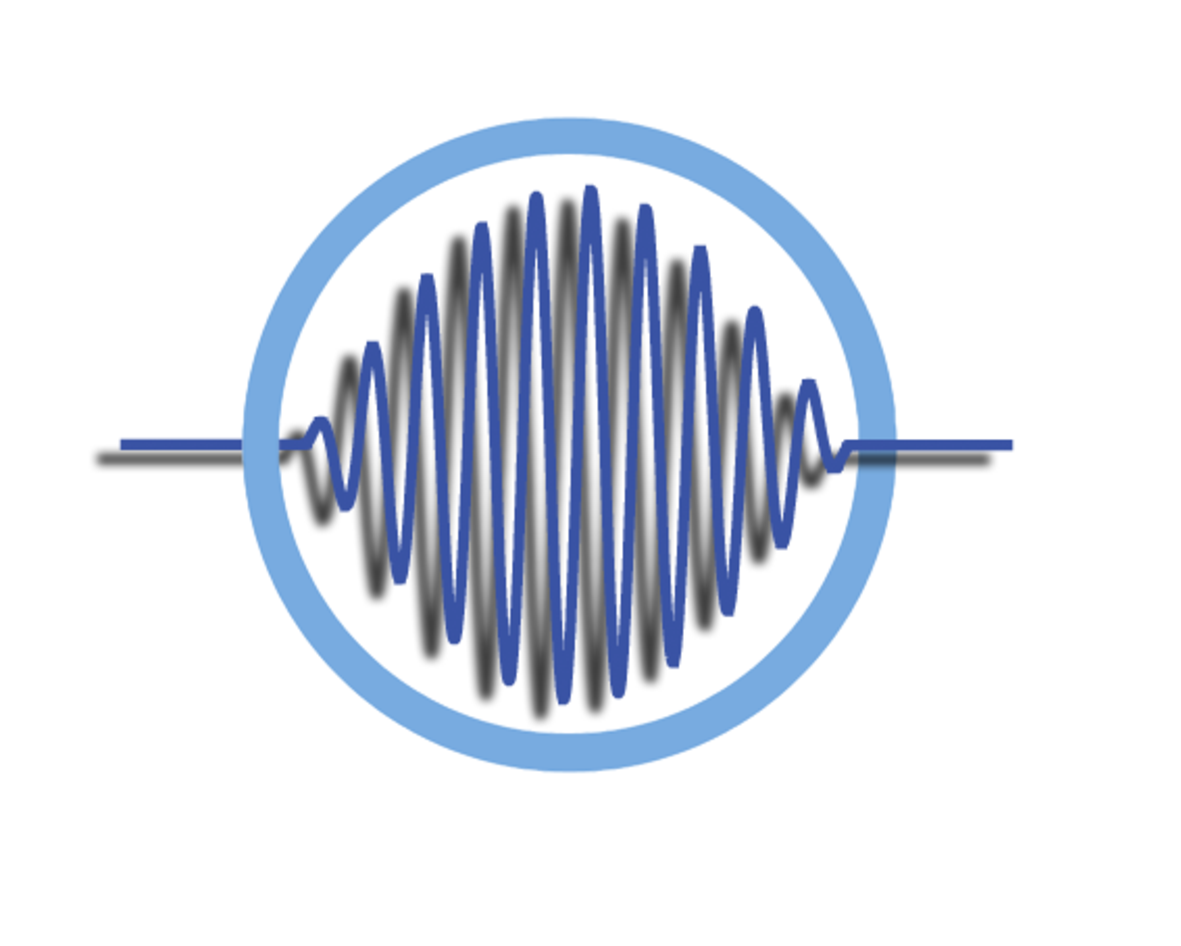
\includegraphics[height=0.18\textheight]{logos/LabDPR_logo} \hspace*{1cm}
  
\includegraphics[height=0.18\textheight,width=0.15\textwidth]{logos/lagologo}

  \titlepage

\end{frame}

\begin{frame}
  \frametitle{Contenido}
  \setcounter{tocdepth}{1} %para incluir solo las secciones en el TOC
  \tableofcontents
%  \tableofcontents[pausesections]
\end{frame}
%
%

%%------------------------------------------------------------------------------
\section{Introducción}
%%------------------------------------------------------------------------------
%\begin{frame}
%  \begin{center}
%    \Huge{\color{blue}{Introducción}} \\
%    \vspace*{5mm}
%    \fbox{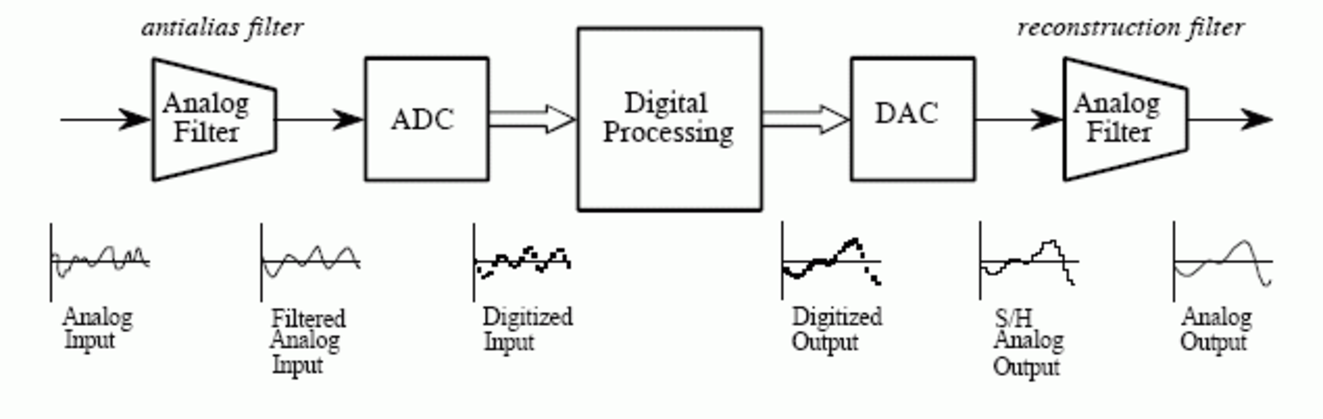
\includegraphics[width=\textwidth]{d3/adc_dac_system_general}}
%  \end{center}
%\end{frame}
%
\begin{frame}
	\frametitle{Introducción}
    \only<1>{\fbox{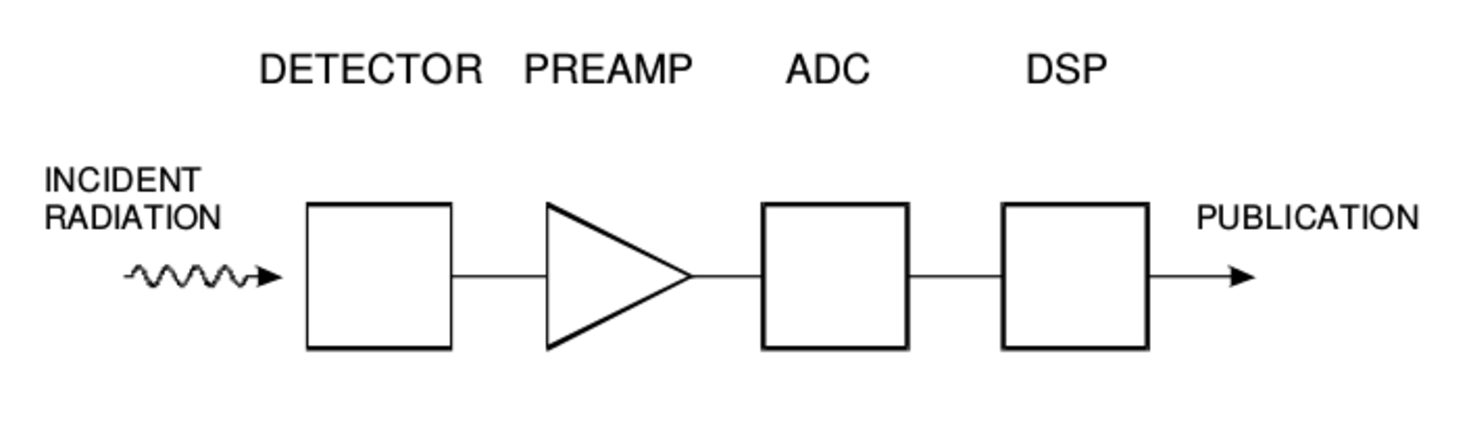
\includegraphics[width=\textwidth]{d1/block_diag_det_syst}}}
    \only<2>{\fbox{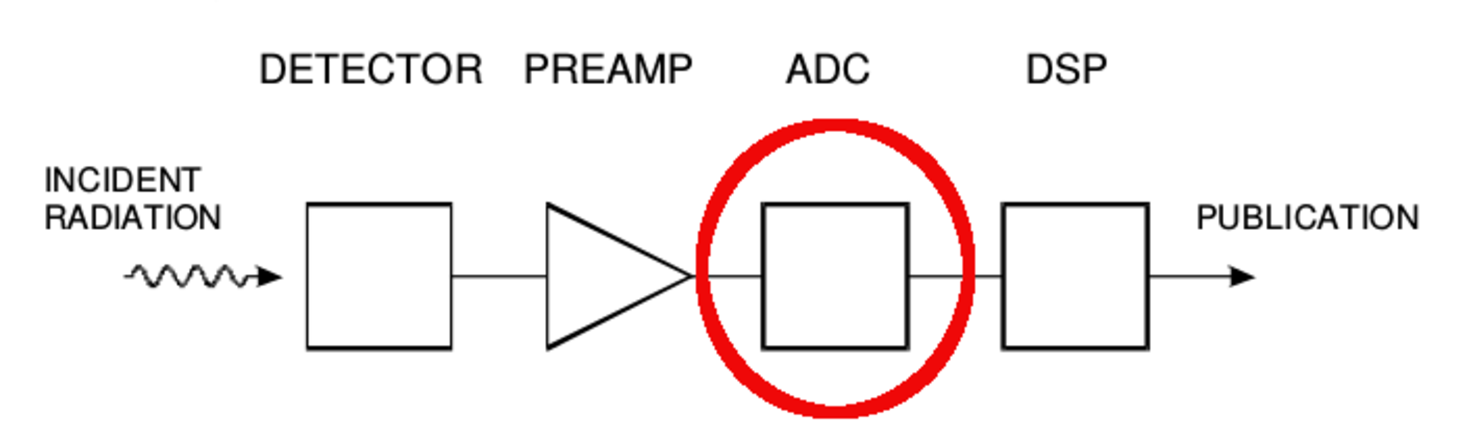
\includegraphics[width=\textwidth]{d1/block_diag_det_syst3}}}
\end{frame}

\begin{frame}
%FIXME: en la intro hablar sobre Nyquist fn = 2* fm, explicar lo que es
%oversampling. Incluir acá las definiciones encontradas en el AN641 de Maxim
%Integrated.
	\frametitle{Definiciones}
		\begin{block}{}
    	\begin{itemize}
      	\item La mayoría de las señales que queremos procesar son analógicas
      	\item es decir son contínuas y pueden tomar infinidad de valores
      	\item Ejemplos:
    	\begin{itemize}
      	\item señal de audio de un micrófono
      	\item señal de salida de un detector de partículas
      	\item voltímetro digital
        \item etc...
    	\end{itemize}
    	\end{itemize}
		\end{block}
\begin{center}
    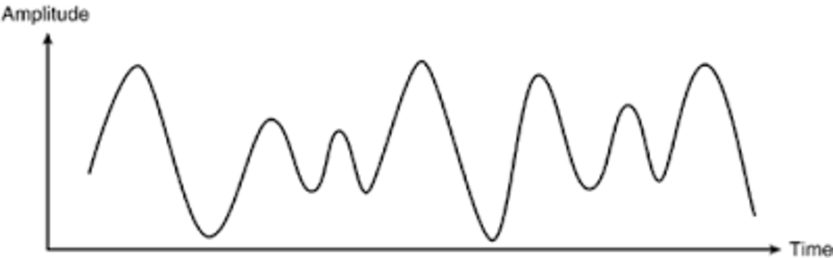
\includegraphics[width=0.5\textwidth]{d3/analog_signal}
\end{center}
\end{frame} 

\begin{frame}
	\frametitle{Definiciones}
{
\setbeamercolor{block body}{bg=red!20, fg=blue}
		\begin{block}{}
    	\begin{itemize}
      	\item Los sistemas digitales requieren datos en formato digital discreto 
      	\item Los ADC convierten información analógica a información digital
      	\item Convertir un pulso analógico en uno digital es muy conveniente en
términos de guardar y analizar la información contenida en la señal  
      	\item Hoy en día los ADC son usados intensamente en todos los sistemas
de detección para convertir los pulsos analógicos en su equivalente digital 
    	\end{itemize}
		\end{block}
}
\begin{center}
    \fbox{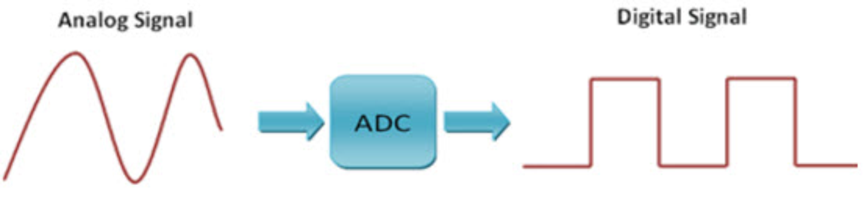
\includegraphics[width=0.6\textwidth]{d3/Analog-to-Digital-Conversion}}
\end{center}
\end{frame} 

\begin{frame}
	\frametitle{Definiciones}
	\framesubtitle{Parámetros relacionados al proceso de conversión A/D}
    	\begin{itemize}
      	\item Tiempo de conversión
      	\item Tiempo muerto
      	\item Resolución
      	\item No-linealidad
      	\item Estabilidad
    	\end{itemize}
\end{frame} 

\begin{frame}
\frametitle{Parámetros relacionados al proceso de conversión A/D}
\begin{block}{Tiempo de conversión}
  	\begin{itemize}
    	\item También conocido como \alert{tiempo de apertura}
    	\item \alert{Se refiere a la incerteza temporal al hacer una conversión y
resulta en una incerteza en la amplitud (o error) en la medición si la señal
cambia durante este tiempo}
    	\item El error puede considerarse como un error en tiempo o en amplitud,
ambos están relacionados:
$$\Delta V = t_a \frac{dV(t)}{dt} \qquad t_a = \text{tiempo de apertura}$$
    	\item $\Delta V$ representa un error máximo, ya que el error real depende
de cómo se hace la conversión
  	\end{itemize}

\end{block}
\end{frame} 

\begin{frame}
\frametitle{Parámetros relacionados al proceso de conversión A/D}
\begin{block}{Tiempo muerto}
  	\begin{itemize}
    	\item Es el tiempo requerido por el ADC para {\color{blue} adquirir la
señal, hacer la conversión y estar disponible para hacer la próxima adquisición} 
    	\item Durante este tiempo el ADC no puede aceptar una señal nueva
    	\item Típicamente compuesto por:
  	\begin{itemize}
    	\item El tiempo de adquisición de señal
    	\item Tiempo de coversión
    	\item Transferencia de datos a el/los buffers
    	\item Tiempo de reset
  	\end{itemize}
    	\item Si la tasa de eventos es tal que los pulsos llegan al ADC durante
este tiempo, la información se pierde 
  	\end{itemize}
\end{block}
\end{frame} 

\begin{frame}
\frametitle{Parámetros relacionados al proceso de conversión A/D}
\begin{block}{Resolución}
  	\begin{itemize}
    	\item La salida del ADC es una \alert{\textit{palabra digital}}, la cual
es simplemente un número 
    	\item {\color{blue} El menor número que el ADC puede asignar a una
entrada analógica determina su resolución} 
    	\item Está expresada en \textit{bits}
    	\item Un ADC de $n$ bits tiene (idealmente) una resolución de 
$$\alert{\frac{\Delta V}{V} = \frac{1}{2^n}}$$
  	\end{itemize}
\end{block}
\end{frame} 

\begin{frame}
\frametitle{Parámetros relacionados al proceso de conversión A/D}
\begin{block}{No-linealidad}
  	\begin{itemize}
    	\item Es uno de los problemas más serios que tienen los ADC
    	\item Depende no solamente del diseño y la circuitería del ADC, sino que
también de la forma y duración de los pulsos analógicos de entrada 
    	\item Hay dos tipos
    	\begin{itemize}
      	\item \textbf{No-linealidad diferencial} $\rightarrow$ mide la uniformidad de los
incrementos del ADC
      	\item \textbf{No-linealidad integral} $\rightarrow$ cuando la salida del ADC no
es linealmente proporcional a la amplitud del pulso de entrada 
    	\end{itemize}
  	\end{itemize}
\end{block}
\end{frame} 

\begin{frame}
\frametitle{Parámetros relacionados al proceso de conversión A/D}
\begin{block}{Estabilidad}
  	\begin{itemize}
    	\item Hace referencia al cambio de las características de conversión del
ADC con el paso del tiempo 
    	\item Es un punto importante a tener en cuenta a la hora de elegir un ADC
para nuestra conversión
  	\end{itemize}
\end{block}
\end{frame} 

\begin{frame}
	\frametitle{Proceso de conversión}
		\begin{block}{3 pasos:}
    	\begin{itemize}
      	\item Muestreo
      	\item Cuantización o cuantificación
      	\item Codificación
    	\end{itemize}
		\end{block}
{
\setbeamercolor{block body}{bg=red!30, fg=blue}
		\begin{block}{}
Todos esos pasos se llevan a cabo en el mismo elemento: \alert{el conversor A/D}
		\end{block}
}
\begin{center}
    \fbox{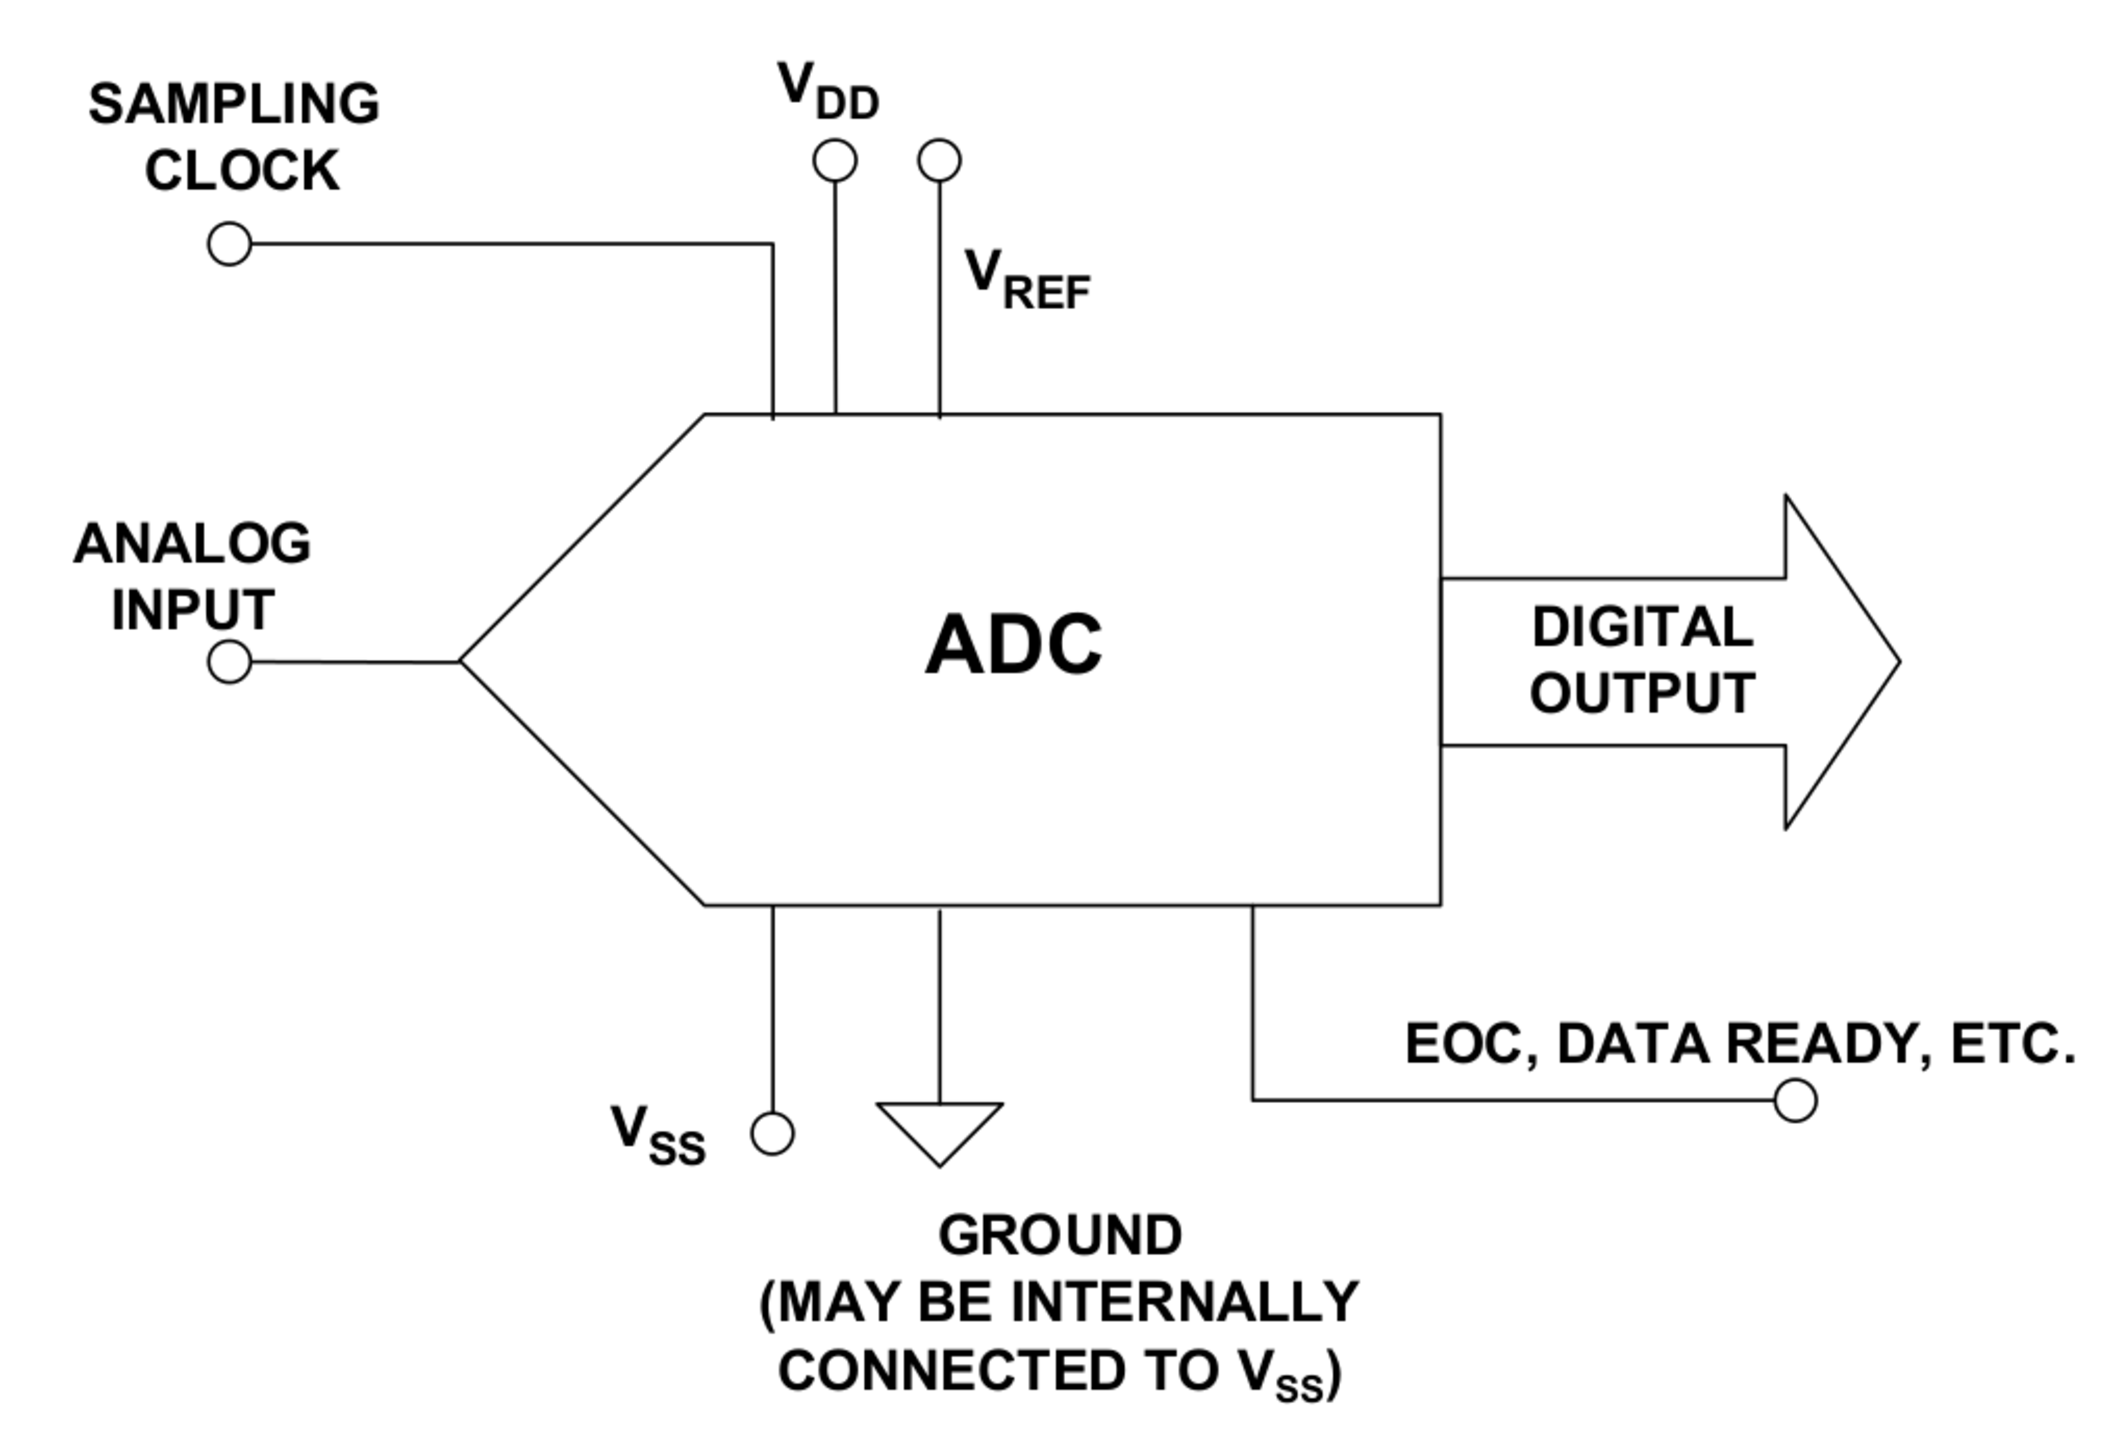
\includegraphics[width=0.4\textwidth]{d3/generic_adc}}
\end{center}
\end{frame} 

\begin{frame}
	\frametitle{Proceso de conversión: Muestreo}
		\begin{block}{}
    	\begin{itemize}
      	\item Los sistemas digitales trabajan con estados discretos
      	\item La señal está definida solamente en determinados momentos
        \item El intervalo de tiempo en el cual se captura la señal se conoce
como la velocidad de muestreo del conversor
      	\item Se debe respetar la frecuencia de Nyquist $\rightarrow f_n = 2f_m$
%muestreo $\rightarrow x_s (t = k*T_s)$
    	\end{itemize}
		\end{block}
{
\setbeamercolor{block body}{bg=red!30, fg=blue}
		\begin{block}{}
En este proceso interviene el circuito de
{\color[rgb]{0.82, 0.1, 0.26} Sample and Hold (S/H)}
		\end{block}
}
\begin{center}
    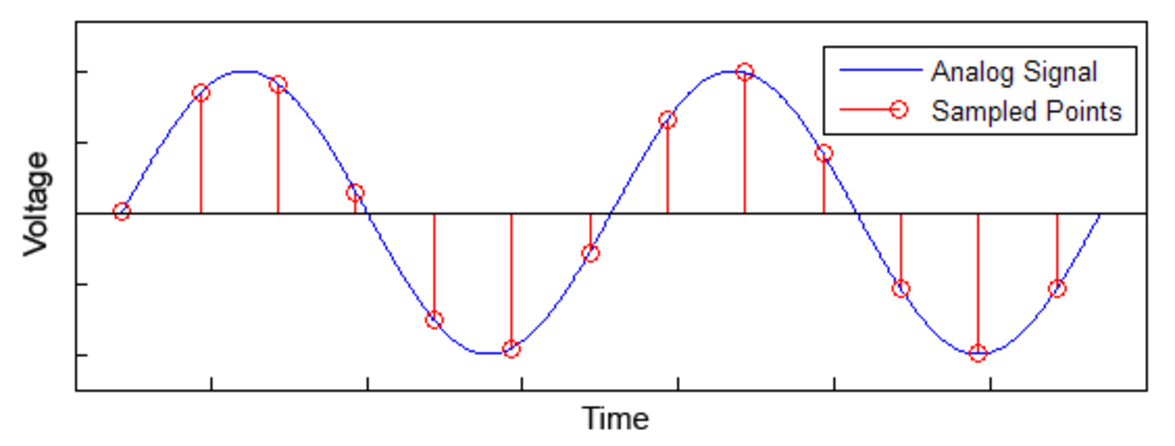
\includegraphics[width=0.6\textwidth]{d3/sampling}
\end{center}
\end{frame} 

\begin{frame}
	\frametitle{Proceso de conversión: cuantización}
		\begin{block}{} 
    	\begin{itemize}
      	\item La señal sólo puede tomar valores determinados, pertenecientes a
un rango de conversión ($\Delta V_r$) 
      	\item Basado en el número de combinaciones de bits que el conversor
puede entregar
      	\item Número de posibles estados: \alert{$N = 2^n$}, donde \alert{n} es el
número de bits
      	\item Resolución: $Q = \Delta V_r / N$
    	\end{itemize}
		\end{block}
{
\setbeamercolor{block body}{bg=green!30, fg=blue}
		\begin{block}{}
Causa lo que se conoce como {\color[rgb]{0.43, 0.21, 0.1} ruido de cuantificación} 
		\end{block}
}
\begin{center}
   \fbox{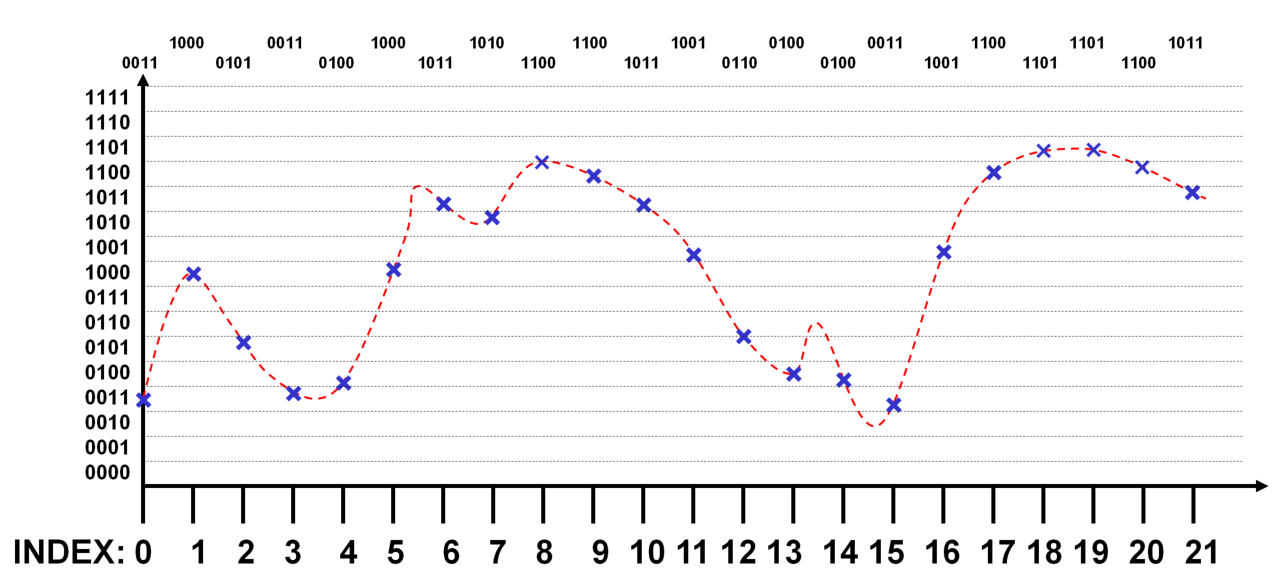
\includegraphics[width=0.4\textwidth]{d3/adc_quantizer}}
\end{center}
\end{frame} 

\begin{frame}
\frametitle{Proceso de conversión: Codificación}
\begin{block}{}
\begin{itemize}
\item Se le asigna una única palabra digital a cada muestra 
\item Haciendo coincidir la palabra digital con la señal de entrada 
\end{itemize}
\end{block}
{
\setbeamercolor{block body}{bg=red!30, fg=blue}
\begin{block}{}
El tipo de codificación usada depende de la aplicación.

De forma general: {\color[rgb]{0.5,.4,0} unipolar} o {\color[rgb]{0.5,.4,0}
bipolar}
\end{block}
}
\begin{center}
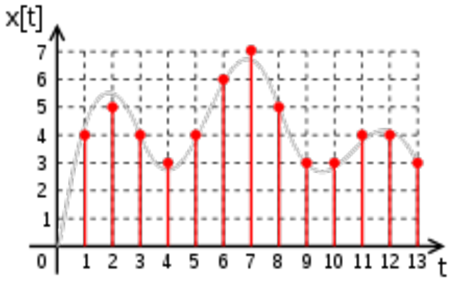
\includegraphics[width=0.4\textwidth]{d3/digital_signal}
\end{center}
\end{frame} 

\begin{frame}
\frametitle{Proceso de conversión: Codificación}
\begin{center}
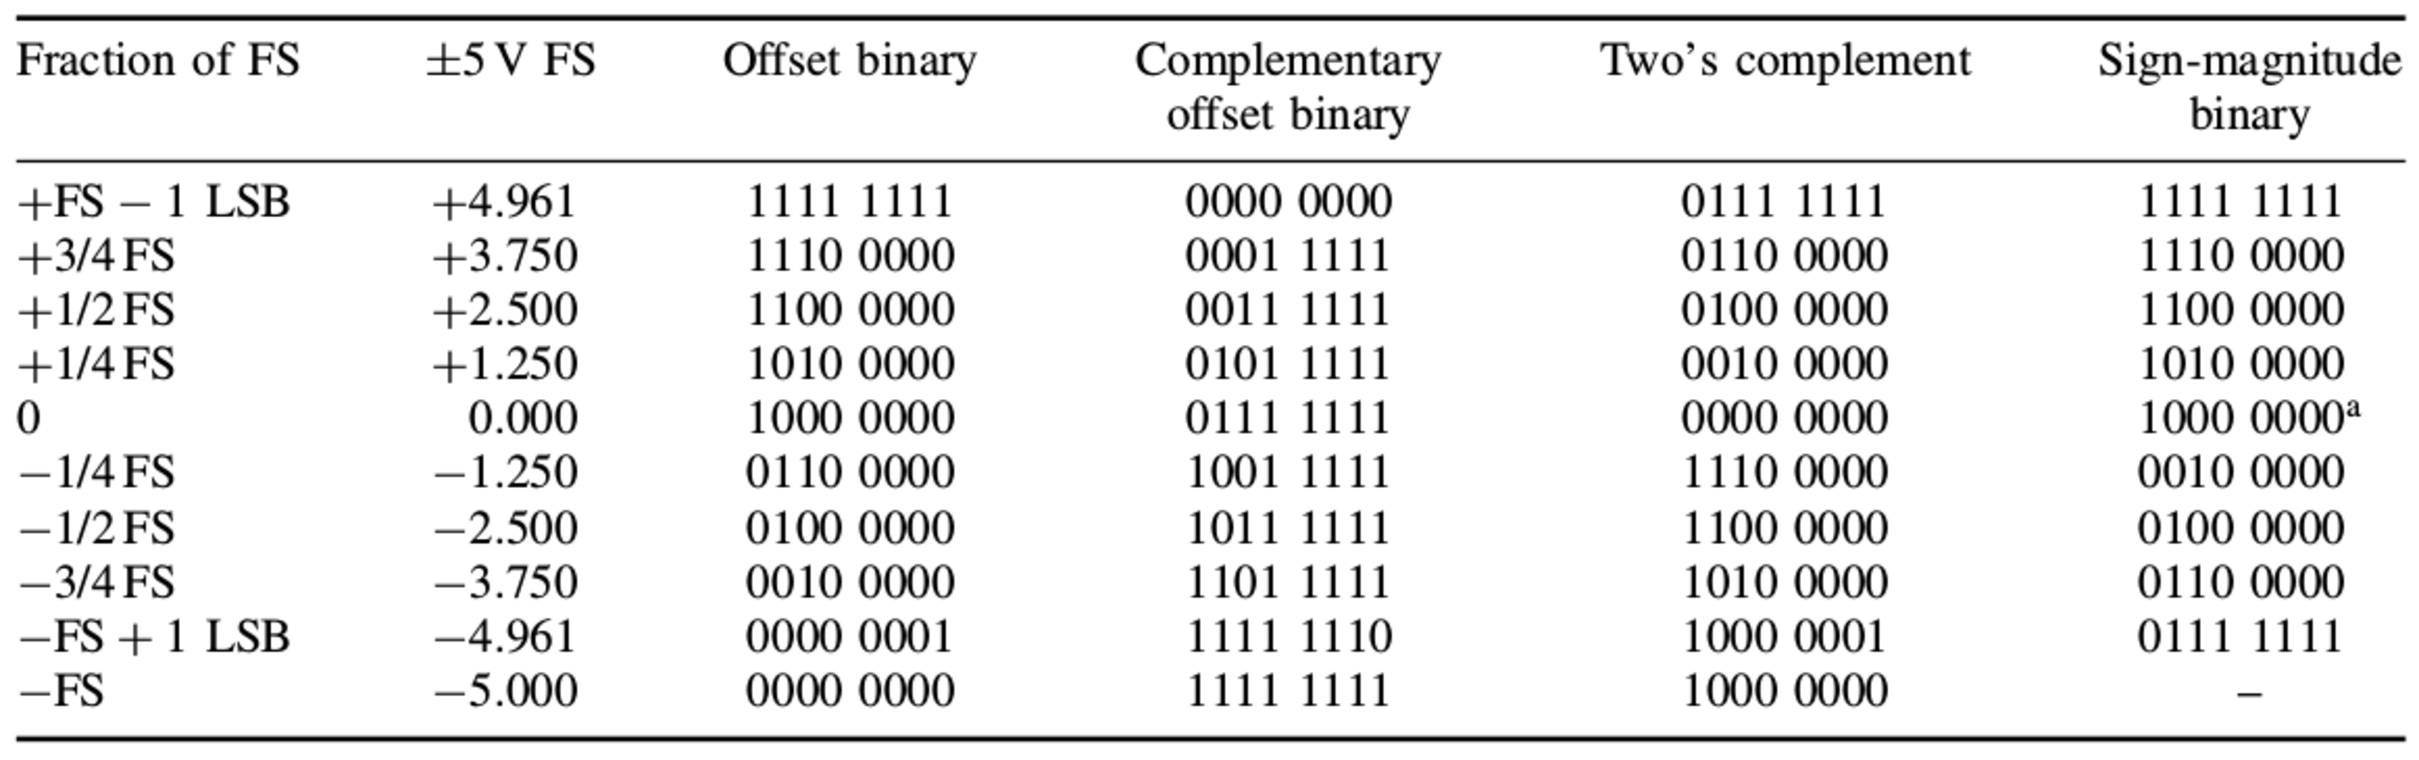
\includegraphics[width=\textwidth]{d3/tabla_codigos_binarios}
\end{center}
\end{frame}

\begin{frame}
\frametitle{Características: rendimientos}
Tabla que resume los rendimientos teóricamente perfectos. 
La tabla muestra, además, la máxima frecuencia de muestreo que actualmente
soportan los mejores dispositivos de cada categoría.
\begin{table}
\begin{tabular}{|p{0.8cm}|p{1.8cm}|p{2cm}|p{2.4cm}|p{2cm}|} \hline
\bf{Res. (bits)} & \bf{Rango (unipolar)} & \bf{Rango (bipolar)} &
\bf{Error de cuantificación} & \bf{Frecuencia Máxima de Muestreo} \\ \hline
    24 & 16,777,216 & $\pm$ 8,388,608 & $\pm$ 0,000003\% & $200\,kHz$  \\
    16 & 65,536     & $\pm$ 32,768    & $\pm$ 0,0008\%   & $250\,MHz$  \\
    14 & 16,384     & $\pm$ 8,192     & $\pm$ 0,003\%    & $400\,MHz$  \\
    12 & 4,096      & $\pm$ 2,048     & $\pm$ 0,012\%    & $1,8\,GHz$  \\
    10 & 1,024      & $\pm$ 512       & $\pm$ 0,05\%     & $2,2\,GHz$  \\
    8  & 256        & $\pm$ 128       & $\pm$ 0,2\%      & $3\,GHz$    \\
    6  & 64         & $\pm$ 32        & $\pm$ 0,8\%      & $6\,GHz$    \\ \hline
\end{tabular}
\end{table}
\end{frame}

\subsection{Parámetros}

\begin{frame}
\frametitle{Parámetros de los conversores A/D}
{
\setbeamercolor{block body}{bg=red!40, fg=blue}
\begin{block}{}
Para poder entender el funcionamiento y el desempeño de un conversor A/D es
necesario que entendamos algunos de los parámetros que los caracterizan 
\end{block}
}
\begin{block}{}
\begin{itemize}
\item Ruido de cuantificación y relación señal a ruido (SNR)
\item Relación señal a ruido y distorsión (SINAD)
\item Número efectivo de bits (ENOB)
\item Distorsión armónica total (THD)
\item Rango dinámico libre de espurios (SFDR)
\item Distorsión por intermodulación de dos tonos (TTIMD)
\item Distorsión por intermodulación multi-tonos (MTIMD)
\item Relación de onda de voltaje estacionario (VSWR)
\end{itemize}
\end{block}
\end{frame} 

\begin{frame}
\frametitle{Ruido de cuantificación}
\framesubtitle{Modelo del ruido de cuantificación}
{
\setbeamercolor{block body}{bg=red!40, fg=blue}
\begin{block}{}
Es importante conocer su origen, ya que la fórmula que lo cuantifica abarca
algunas sutilezas que, si no se entienden, pueden conducir a una
\alert{interpretación errónea} tanto de las especificaciones de la hoja de datos como del
desempeño de conversor A/D
\end{block}
}
\begin{block}{}
\begin{itemize}
\item El ruido de cuantificación y el SNR están íntimamente relacionados 
\item Establece lo que se conoce como \alert{piso de ruido} para la
conversión
\item El valor teórico máximo para el SNR se define a partir de este
modelo 
\end{itemize}
\end{block}
\end{frame} 

\begin{frame}
\frametitle{Ruido de cuantificación}
\framesubtitle{Modelo del ruido de cuantificación}
{
\setbeamercolor{block body}{bg=blue!40, fg=white}
\begin{block}{}
El error máximo que se comete al realizar la conversión con un conversor ideal
es de $\pm\,1/2\,LSB$ ($Q = 1\,LSB$)
		\end{block}
}
\begin{center}
\fbox{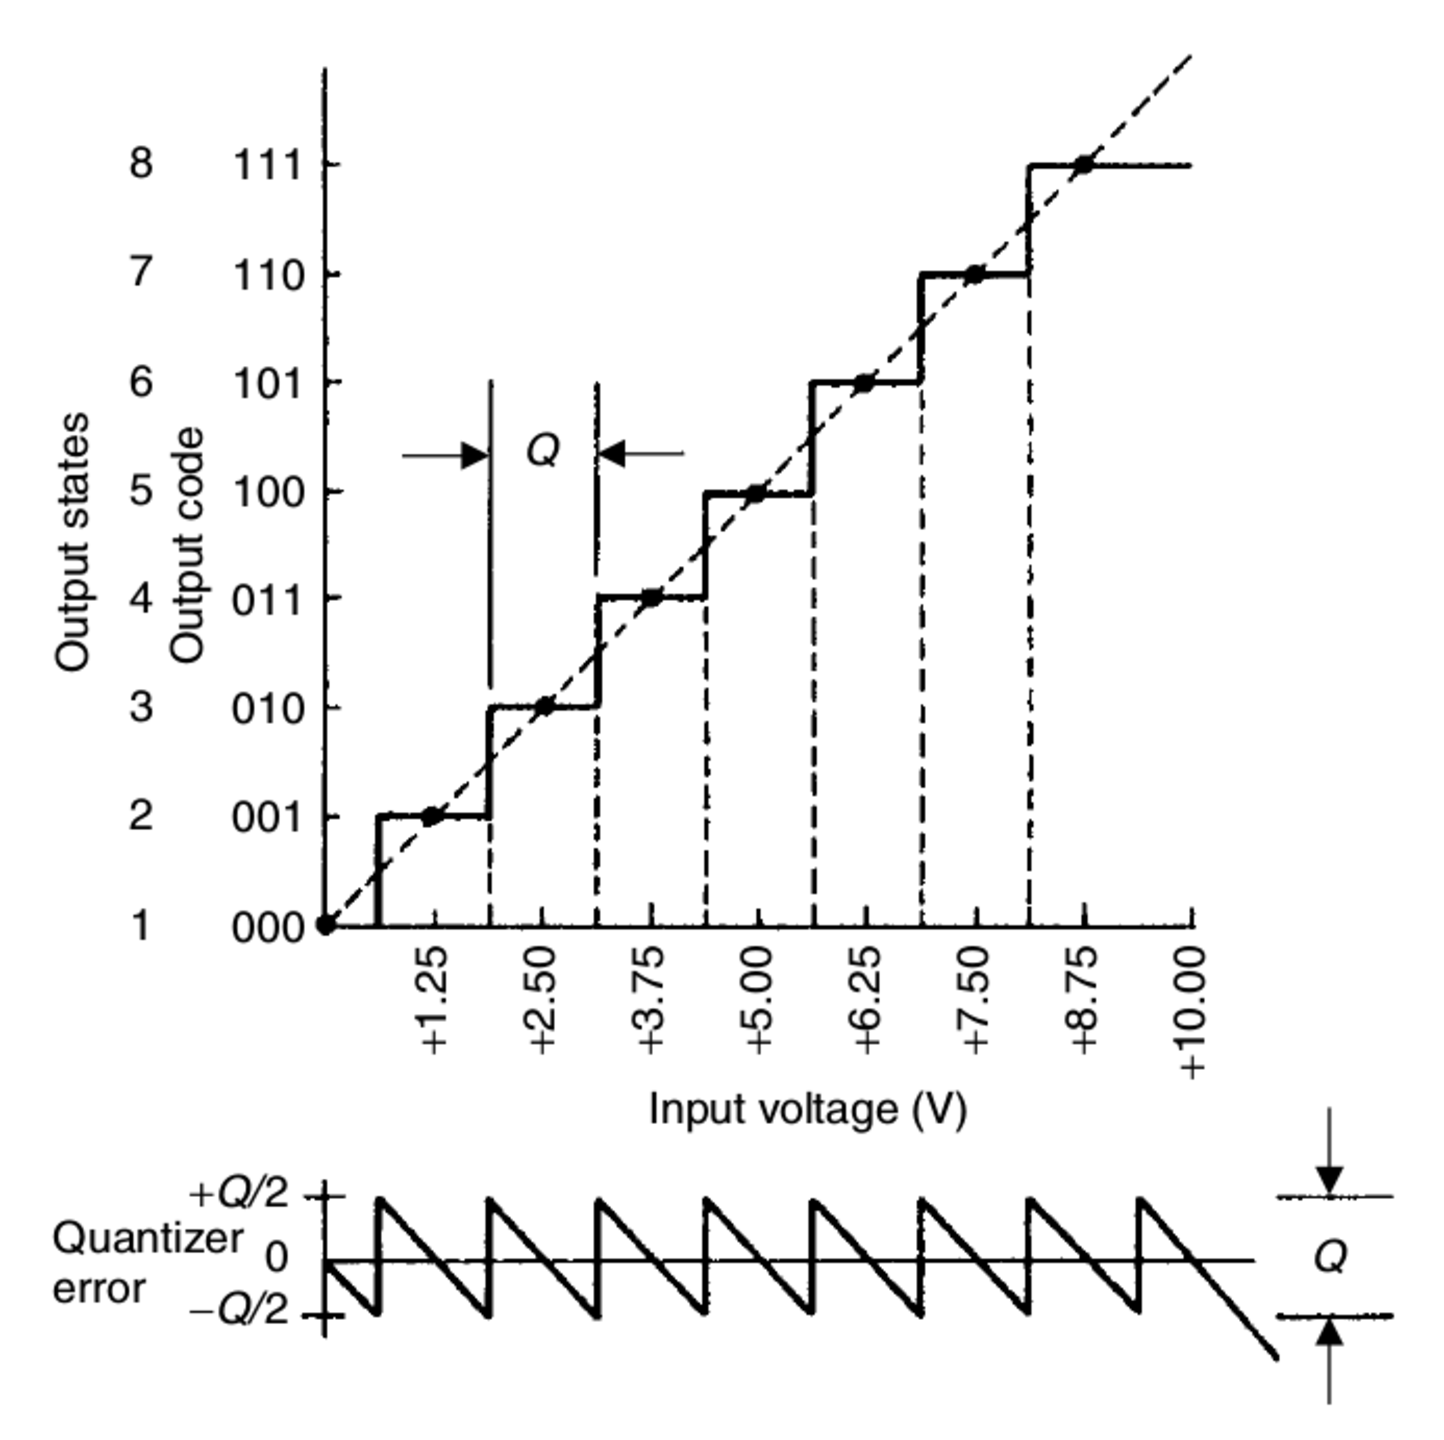
\includegraphics[width=.4\textwidth]{d3/quantization_error1}}
\end{center}
\end{frame} 

%\begin{frame}
%\frametitle{Parámetros: \alert{SNR}}
%\begin{block}{}
%\begin{itemize}
%\item Sistema todo-en-uno
%\item Guardar los datos para futuros análisis (off-line data analysis)
%en un lugar centralizado y de fácil acceso para toda la
%Colaboración
%\item Uniformizar el formato de los datos/archivos guardados
%\end{itemize}
%\end{block}
%\end{frame} 
%
%\begin{frame}
%\frametitle{Parámetros: \alert{ENOB}}
%\begin{block}{}
%\begin{itemize}
%\item Sistema todo-en-uno
%\item Guardar los datos para futuros análisis (off-line data analysis)
%en un lugar centralizado y de fácil acceso para toda la
%Colaboración
%\item Uniformizar el formato de los datos/archivos guardados
%\end{itemize}
%\end{block}
%\end{frame} 

%\begin{frame}
%	\frametitle{Definiciones (Cont.)}
%	%\frametitle{Los inicios}
%		\begin{columns}
%			\begin{column}{0.50\textwidth}
%				\begin{block}{Electrónica dedicada para Auger}
%		    	\begin{itemize}
%\item Poco flexible 
%\item Información limitada
%\item Número limitado de UBs (\alert{Unified Boards})
%\item Comunicación de datos por puerto serie
%\item	Tiempos de adquisición largos
%\item	Poco volumen de almacenamiento
%\item Sin control línea de base	
%\end{itemize}
%\end{block}
%			\end{column} 
%		 	\begin{column}{0.50\textwidth}
%		  	%\fbox{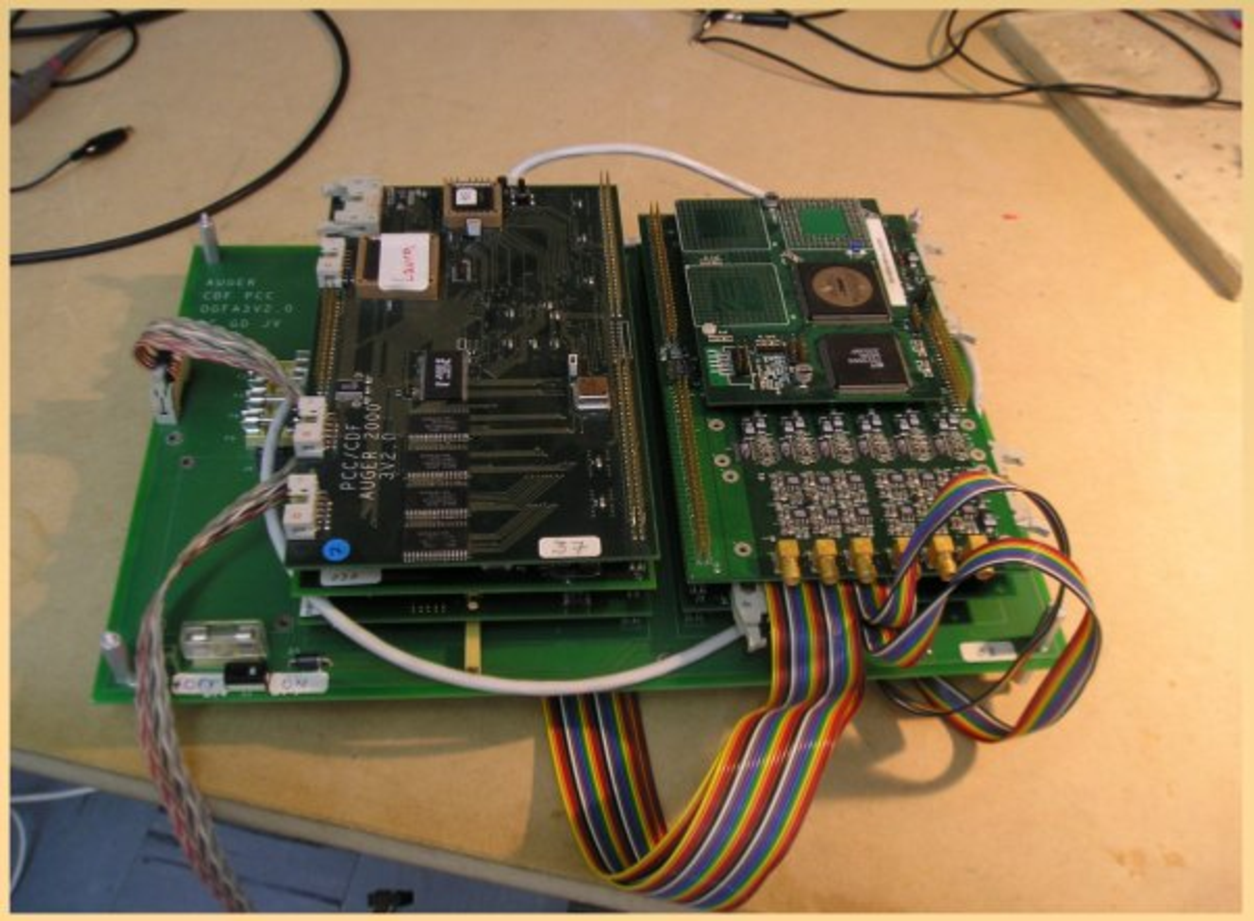
\includegraphics[width=\textwidth]{d3/electronica_auger}}
%		 \end{column}
%		\end{columns}
%\end{frame} 
%
%\begin{frame}
%	\frametitle{Actualidad: ¿con qué contamos?}
%	\begin{columns}
%		\begin{column}{0.40\textwidth}
%			\begin{block}{}
%	    	\begin{itemize}[<+->]
%	      	\item Placas de digitalización de 3 y 4 canales
%	      	\item GPS para sincronizar los datos de los 
%								distintos sitios
%	      	\item Barómetro y sensor de temperatura
%					\item Placa Nexys2 (FPGA Spartan 3E)
%	    	\end{itemize}
%			\end{block}
%		\end{column} 
%	 	\begin{column}{0.55\textwidth}
%	  	%\only<1-2>{\fbox{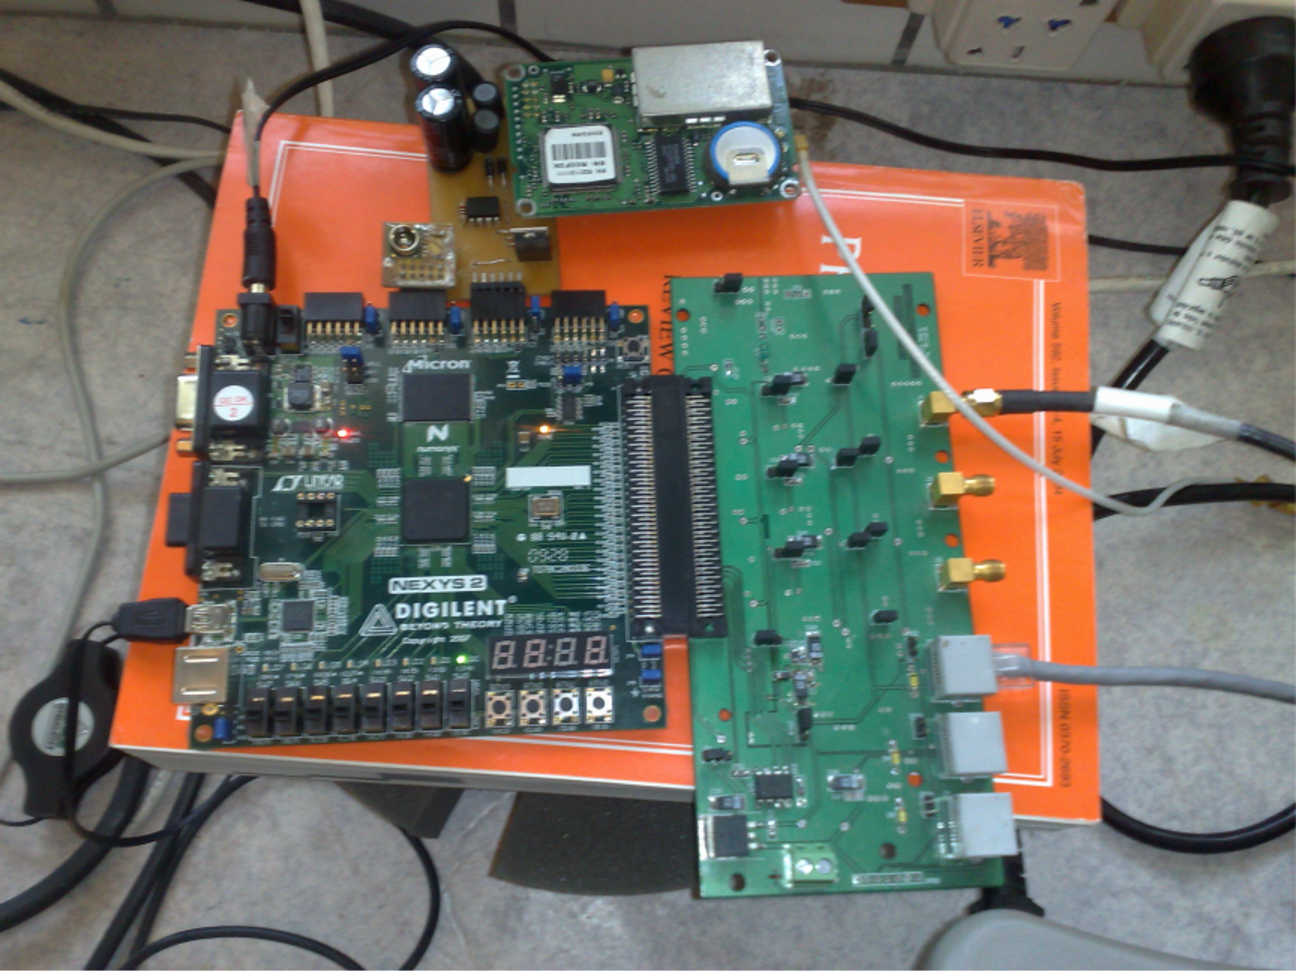
\includegraphics[width=\textwidth]{d3/hardware_nahuelito}}}
%	  	%\only<3-4>{\fbox{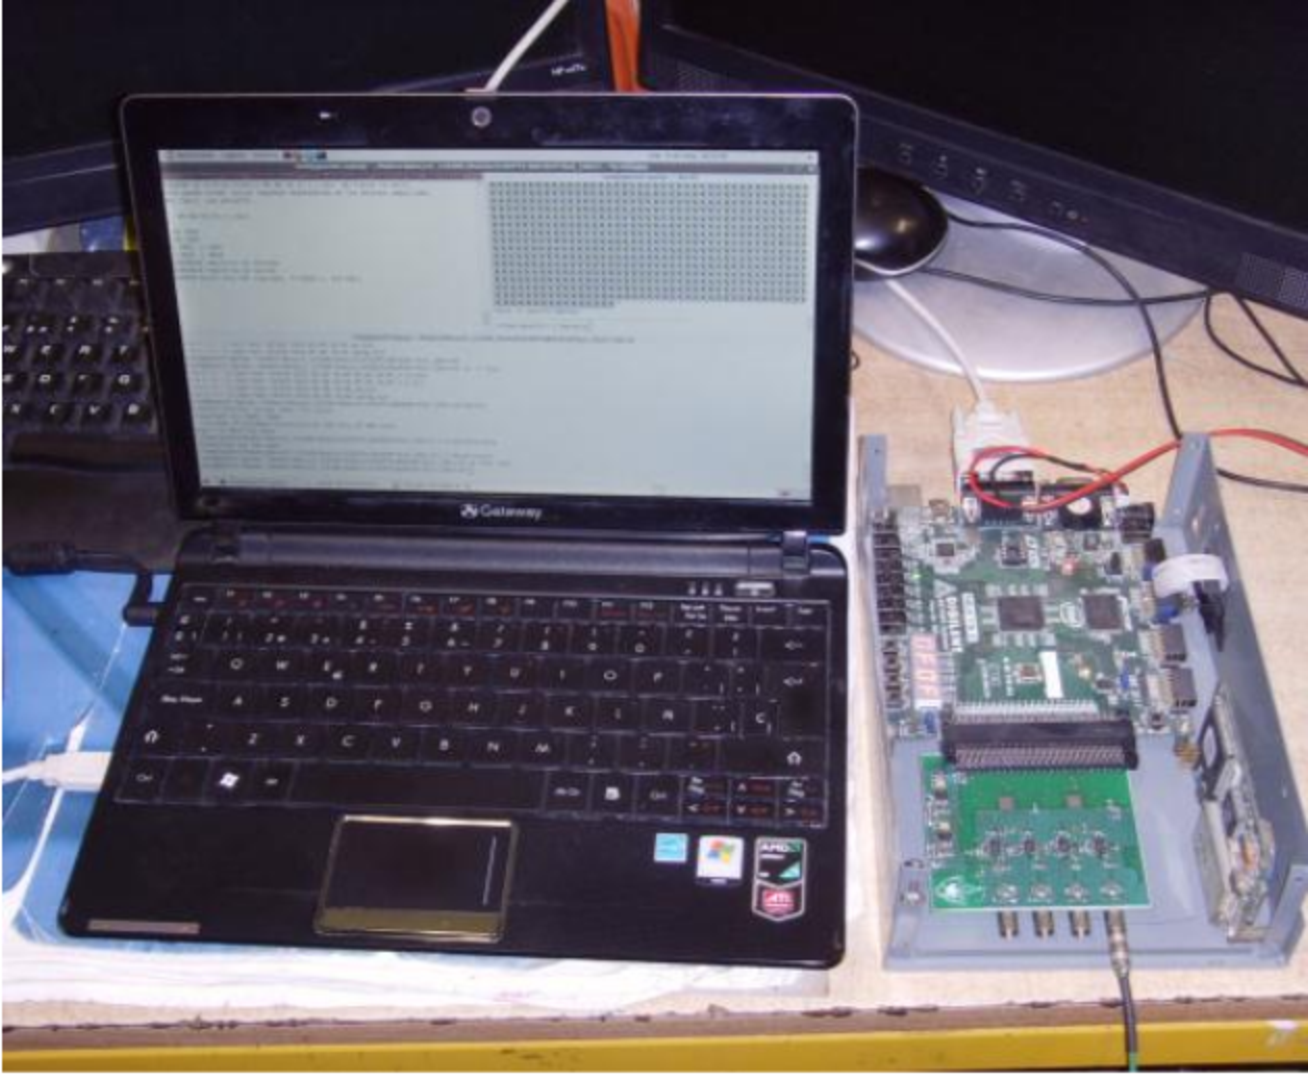
\includegraphics[width=\textwidth]{d3/placa_mx_2}}}
%	 \end{column}
%	\end{columns}
%\end{frame} 
%
%\begin{frame}
%	\frametitle{Dificultades actuales}
%	\begin{alertblock}{}
%		\begin{itemize}
%		\item Hasta la aparición del sistema \alert{ACQUA}, \alert{ANNA}, etc
%					(aprox. noviembre de 2015) teníamos (casi) cada sitio una versión
%					diferente del \alert{firmware} de la FPGA 
%		\item No todos los sitios pueden estar online con sus datos (por diversas
%					razones, a veces ajenas a la electrónica)
%		\item Existencia de dos tipos de electrónicas (con características muy
%					diferentes)
%		\item Problemas contínuos con las placas de adquisición (cortos, falsos
%					contactos, soldaduras frías, etc) debido a que se ensamblan en casa
%		\end{itemize}
%	\end{alertblock}
%\end{frame} 
%
%\begin{frame}
%	\frametitle{Dificultades actuales}
%	\begin{alertblock}{}
%		\begin{itemize}
%		\item Los GPS Oncore están dejando de funcionar en casi todos los sitios y
%					nosotros tenemos la electrónica dedicada a ese GPS particular (que ya no se
%					fabrica más, además)
%		\item Sensores de PyT (HP03) difíciles de conseguir hoy en día
%		\item Las placas Nexys2 \alert{¡dejaron de fabricarse!} y constituyen el
%					corazón de lo que tenemos actualmente
%		\item ...todo tiene un final, todo termina...
%		\end{itemize}
%	\end{alertblock}
%\end{frame} 
%
%\begin{frame}
%	\frametitle{Futuro: ¿cuál es la opción?}
%	\begin{columns}
%		\begin{column}{0.40\textwidth}
%			\begin{block}{}
%	    	\begin{itemize}[<+->]
%	      	\item RedPitaya: 2 canales @ 50\,MHz (adquisición)
%	      	\item Capacidad de conexión y envío de datos a puntos remotos
%	      	\item Se pueden conectar los sensores que necesitemos 
%					\item Mucha \alert{flexibilidad} (¡justo lo que queremos!)
%	    	\end{itemize}
%			\end{block}
%		\end{column} 
%	 	\begin{column}{0.55\textwidth}
%	  	%\fbox{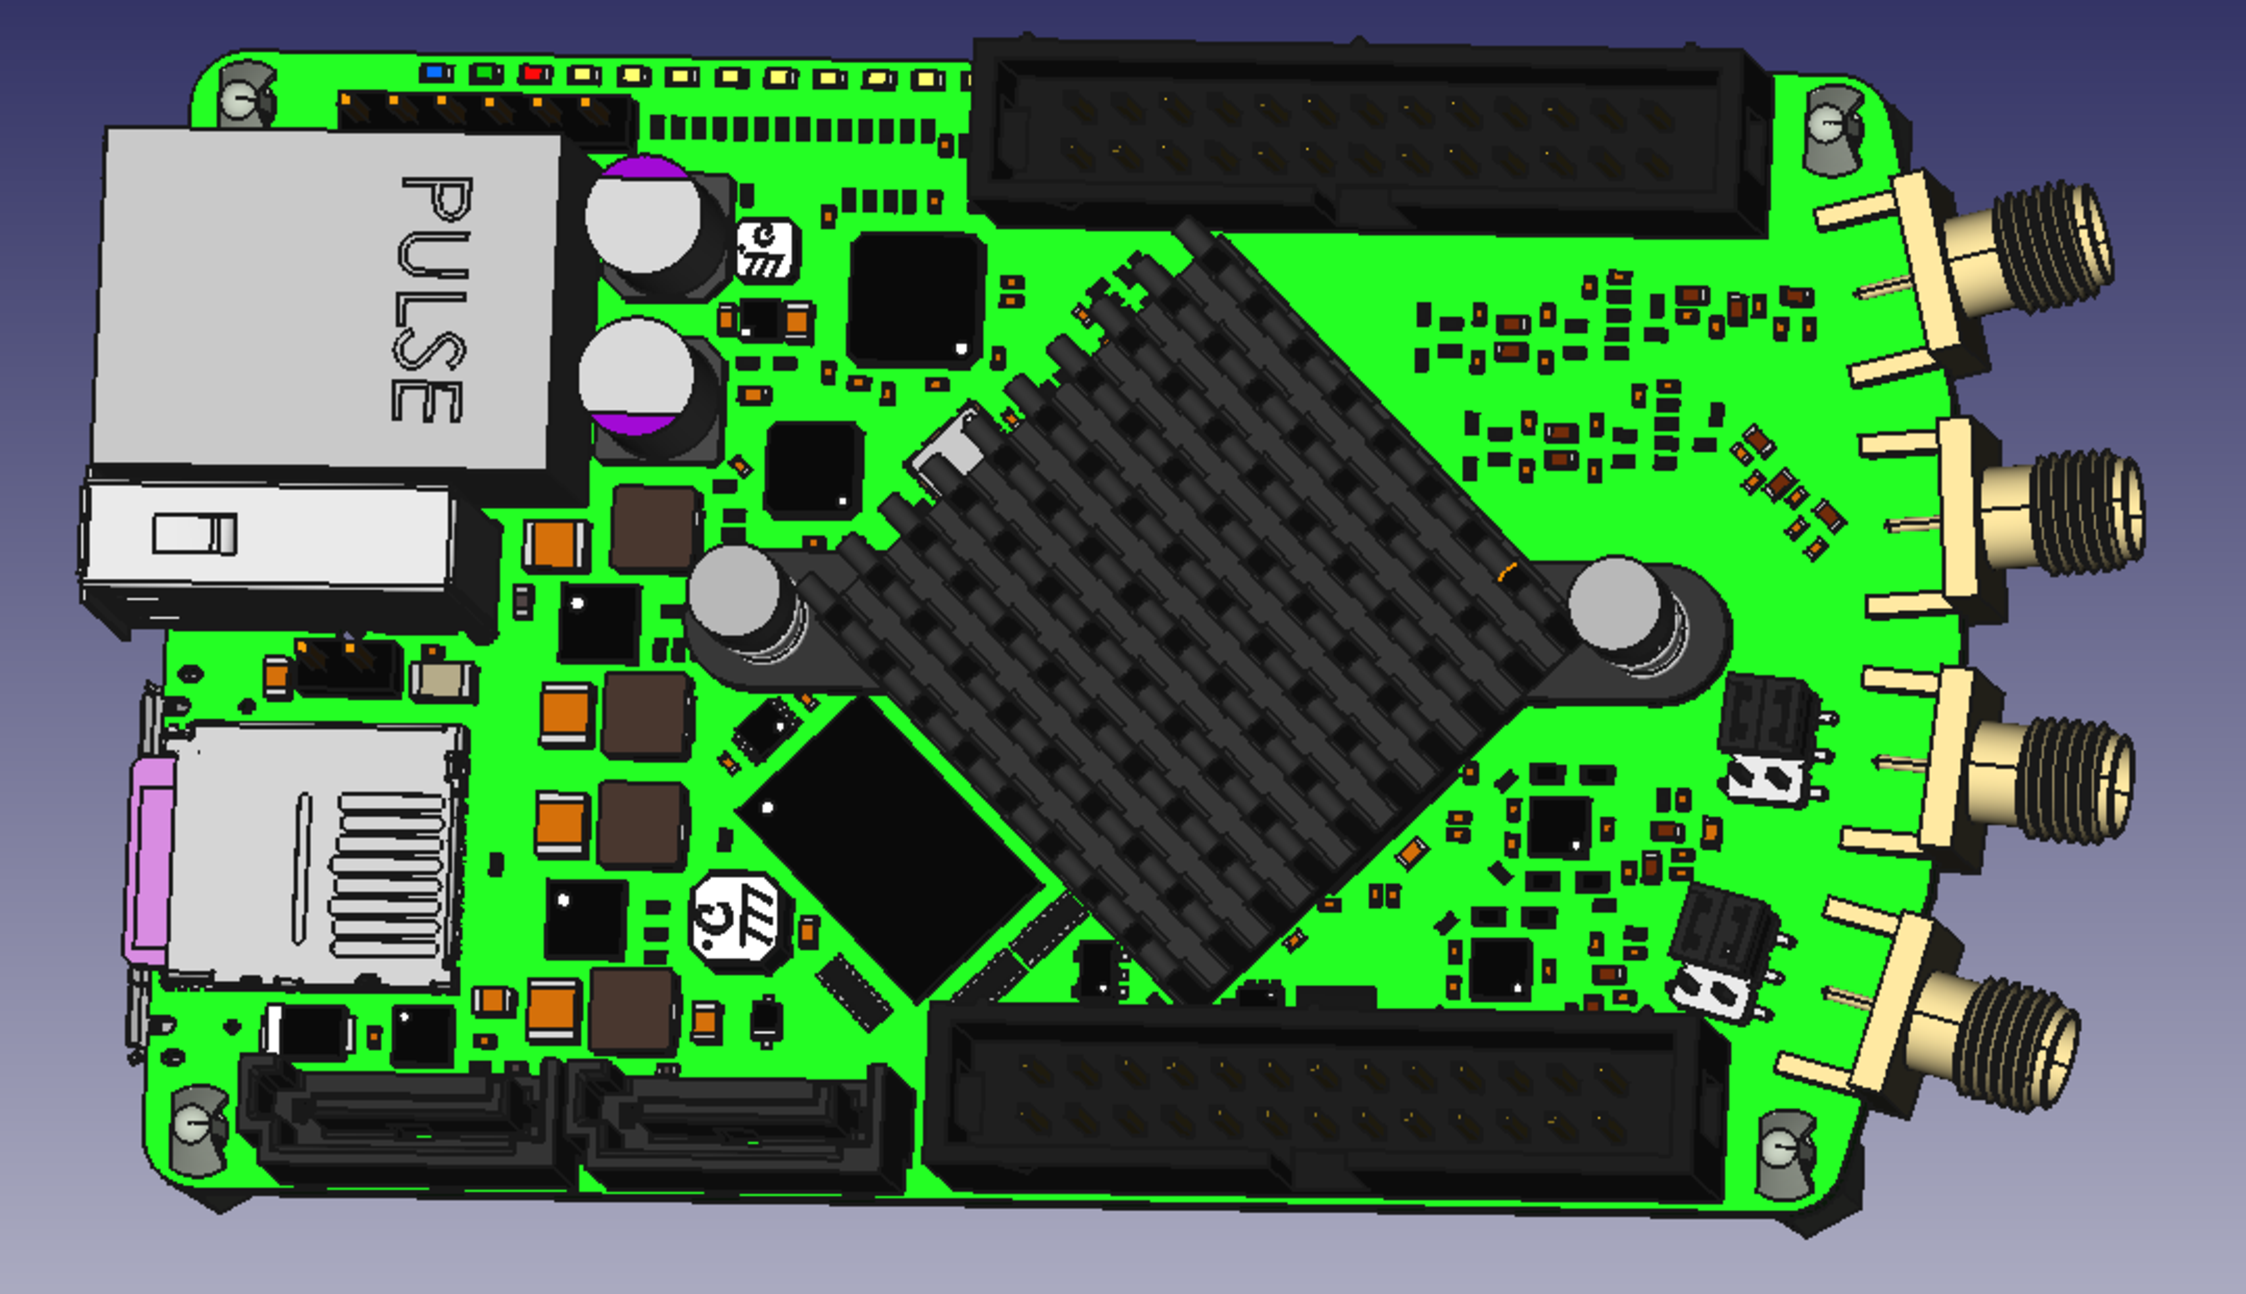
\includegraphics[width=\textwidth]{d3/rp_freecad_up}}
%	 \end{column}
%	\end{columns}
%\end{frame} 
%
%\begin{frame}
%	\frametitle{Futuro: RedPitaya}
%		\begin{block}{}
%	  	\begin{itemize}
%	    	\item Esperamos tener el sistema listo para fin de año (2016) o mediados
%							del año que viene
%	    	\item Es poca la ganancia en ancho de banda, respecto a lo que ya
%							tenemos. Pero se gana mucho en flexibilidad.
%	    	\item Todavía hay que trabajar, tanto en hardware como en software
%				\item ... pero para eso estamos dentro de una comunidad... y el \alert{trabajo
%							colaborativo} debe afianzarse
%	  	\end{itemize}
%		\end{block}
%\end{frame} 
%

%------------------------------------------------------------------------------
\section{ADC}
%------------------------------------------------------------------------------

\begin{frame}
\begin{center}
\Huge{\color{blue}{Conversores analógico a digital (ADC)}} 

\fbox{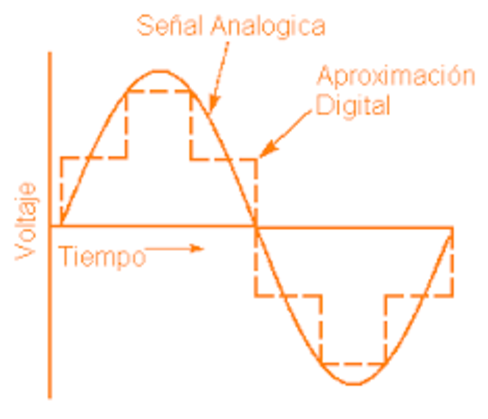
\includegraphics[height=0.5\textheight, width=0.5\textwidth]{d3/adc_generico}}
\end{center}
\end{frame}

\begin{frame}
\frametitle{Conversores analógico a digital (A/D)}
\begin{alertblock}{}
Dispositivo electrónico que transforma un voltaje analógico a un
número binario (series de 1's y 0's) y luego, eventualmente a un número digital
(base 10) para su lectura en un medidor o monitor 
\end{alertblock}
\begin{exampleblock}{}
\begin{itemize}
\item El número de dígitos binarios (bits) que representa el número digital
determina la resolución de ADC
\item El número digital es sólo una \alert{aproximación} del valor verdadero
de la tensión analógica en un instante particular porque el voltaje sólo
puede ser representado (digitalmente) en pasos discretos
\item El grado de aproximación al valor analógico depende también de la
resolución del ADC
\end{itemize}
\end{exampleblock}
\end{frame} 

\begin{frame}
\frametitle{Conversores analógico a digital (A/D)}
\begin{alertblock}{}
Resolución \alert{teórica}: un ADC de
{\color{blue} n} bits tiene una resolución de una parte en {\color{blue} $2^n$}
\end{alertblock}
\begin{exampleblock}{Ejemplo}
\begin{itemize}
\item Un ADC de 12 bits tiene una resolución de una parte en 4096, donde
$2^{12} = 4096$
\item Entonces, un ADC de 12 bits con una entrada máxima de $10\,V_{DC}$
puede resolver la medición en $10\,V_{DC}/4096 = 0.00244\,V_{DC} = 2.44\, mV$
\item {\color{blue} La resolución se especifica normalmente con respecto al rango completo
de lectura, no con respecto al valor medido en algún instante particular}
\end{itemize}
\end{exampleblock}
\end{frame} 

\subsection{Tipos de ADC}

\begin{frame}
\frametitle{Tipos de ADC}
\begin{exampleblock}{Ejemplo}
\begin{itemize}
\item ADC Flash
\item ADC de aproximaciones sucesivas
\item ADC conversor de voltaje a frecuencia 
\item ADC de doble envolvente 
\item ADC sigma-delta
\end{itemize}
\end{exampleblock}
\end{frame} 

\subsubsection{ADC Flash}

\begin{frame}
\frametitle{ADC Flash}
\begin{columns}
\begin{column}{0.65\textwidth}
\begin{block}{}
\begin{itemize}
\item  También conocido como \textbf{ADC paralelo}
\item  \alert{Es la forma más rápida de convertir una señal analógica a
digital}
          \item  Especial para cuando se requiere gran ancho de banda 
          \item  Consume mucha potencia (relativo)
          \item  Tienen poca resolución (relativo)
          \item  Pueden tener un costo excesivo (relativo)
\end{itemize}
\end{block}
\end{column} 
\begin{column}{0.35\textwidth}
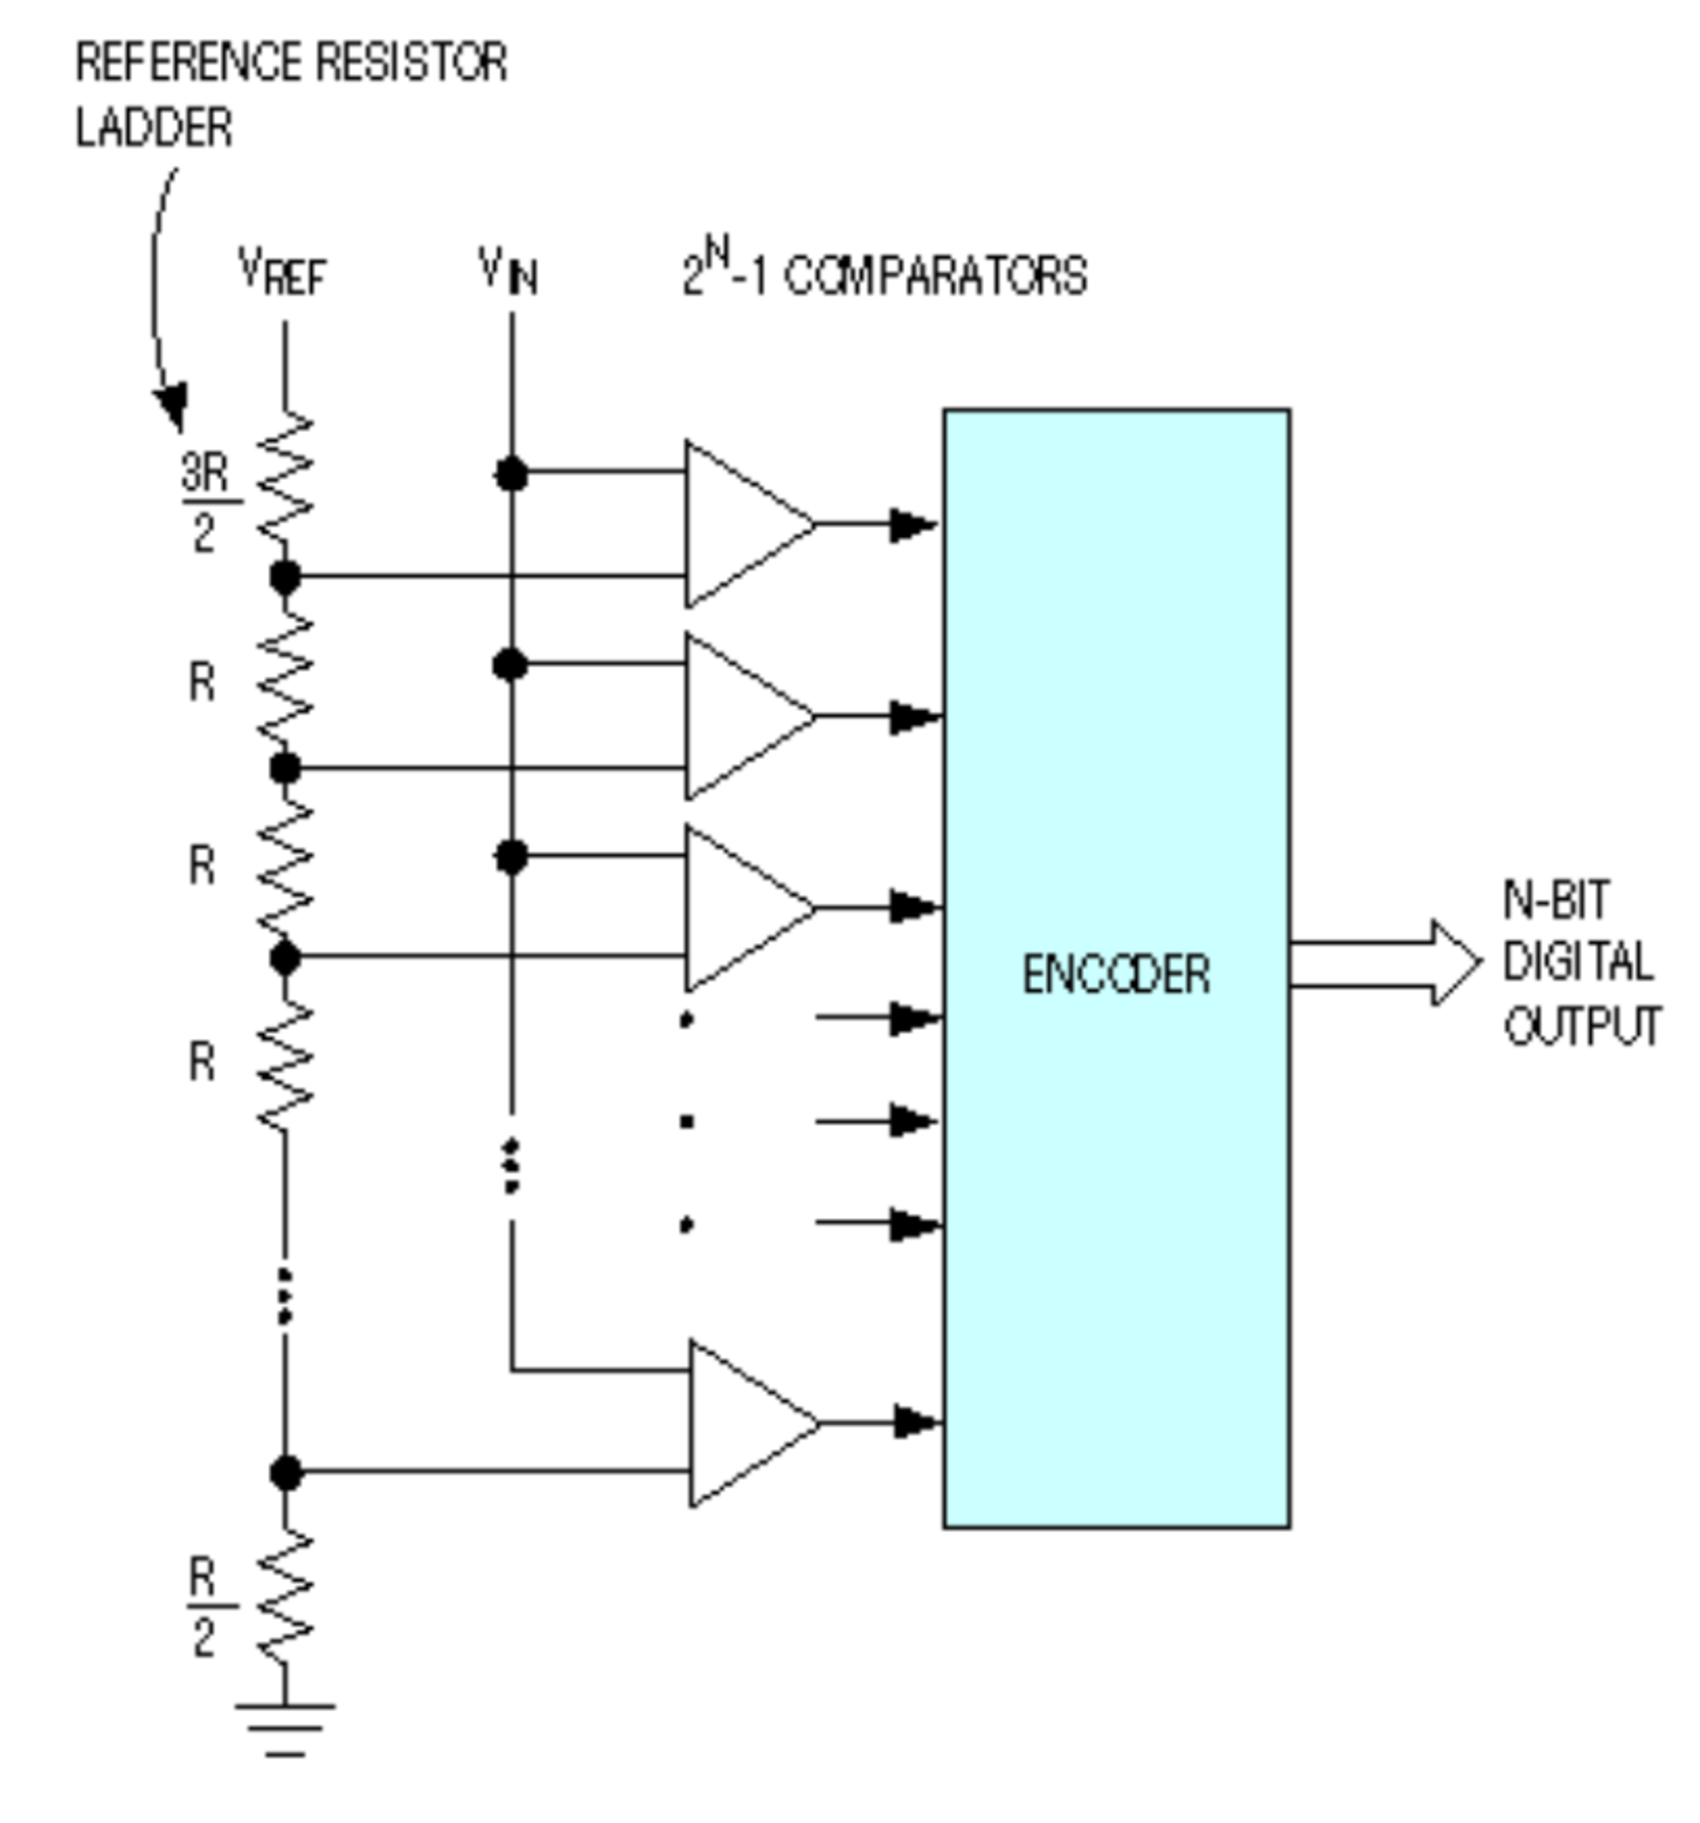
\includegraphics[height=0.5\textheight,width=0.9\textwidth]{d3/adc_flash}
\end{column}
\end{columns}
      \begin{alertblock}{}
          {\color{blue}Limitados a aplicaciones de altas frecuencias en las que
la conversión A/D no puede hacerse de otra forma}%FIXME: esto colocarlo en un
%recuadro como resaltándolo.
      \end{alertblock}
\end{frame}

\begin{frame}
\frametitle{ADC Flash}
  \begin{columns}
    \begin{column}{0.40\textwidth}
      \begin{block}{}
        \begin{itemize}
          \item  Uno de los usos de los amplificadores operacionales (AO) es como comparador
        \end{itemize}
      \end{block}
    \end{column} 
    \begin{column}{0.60\textwidth}
      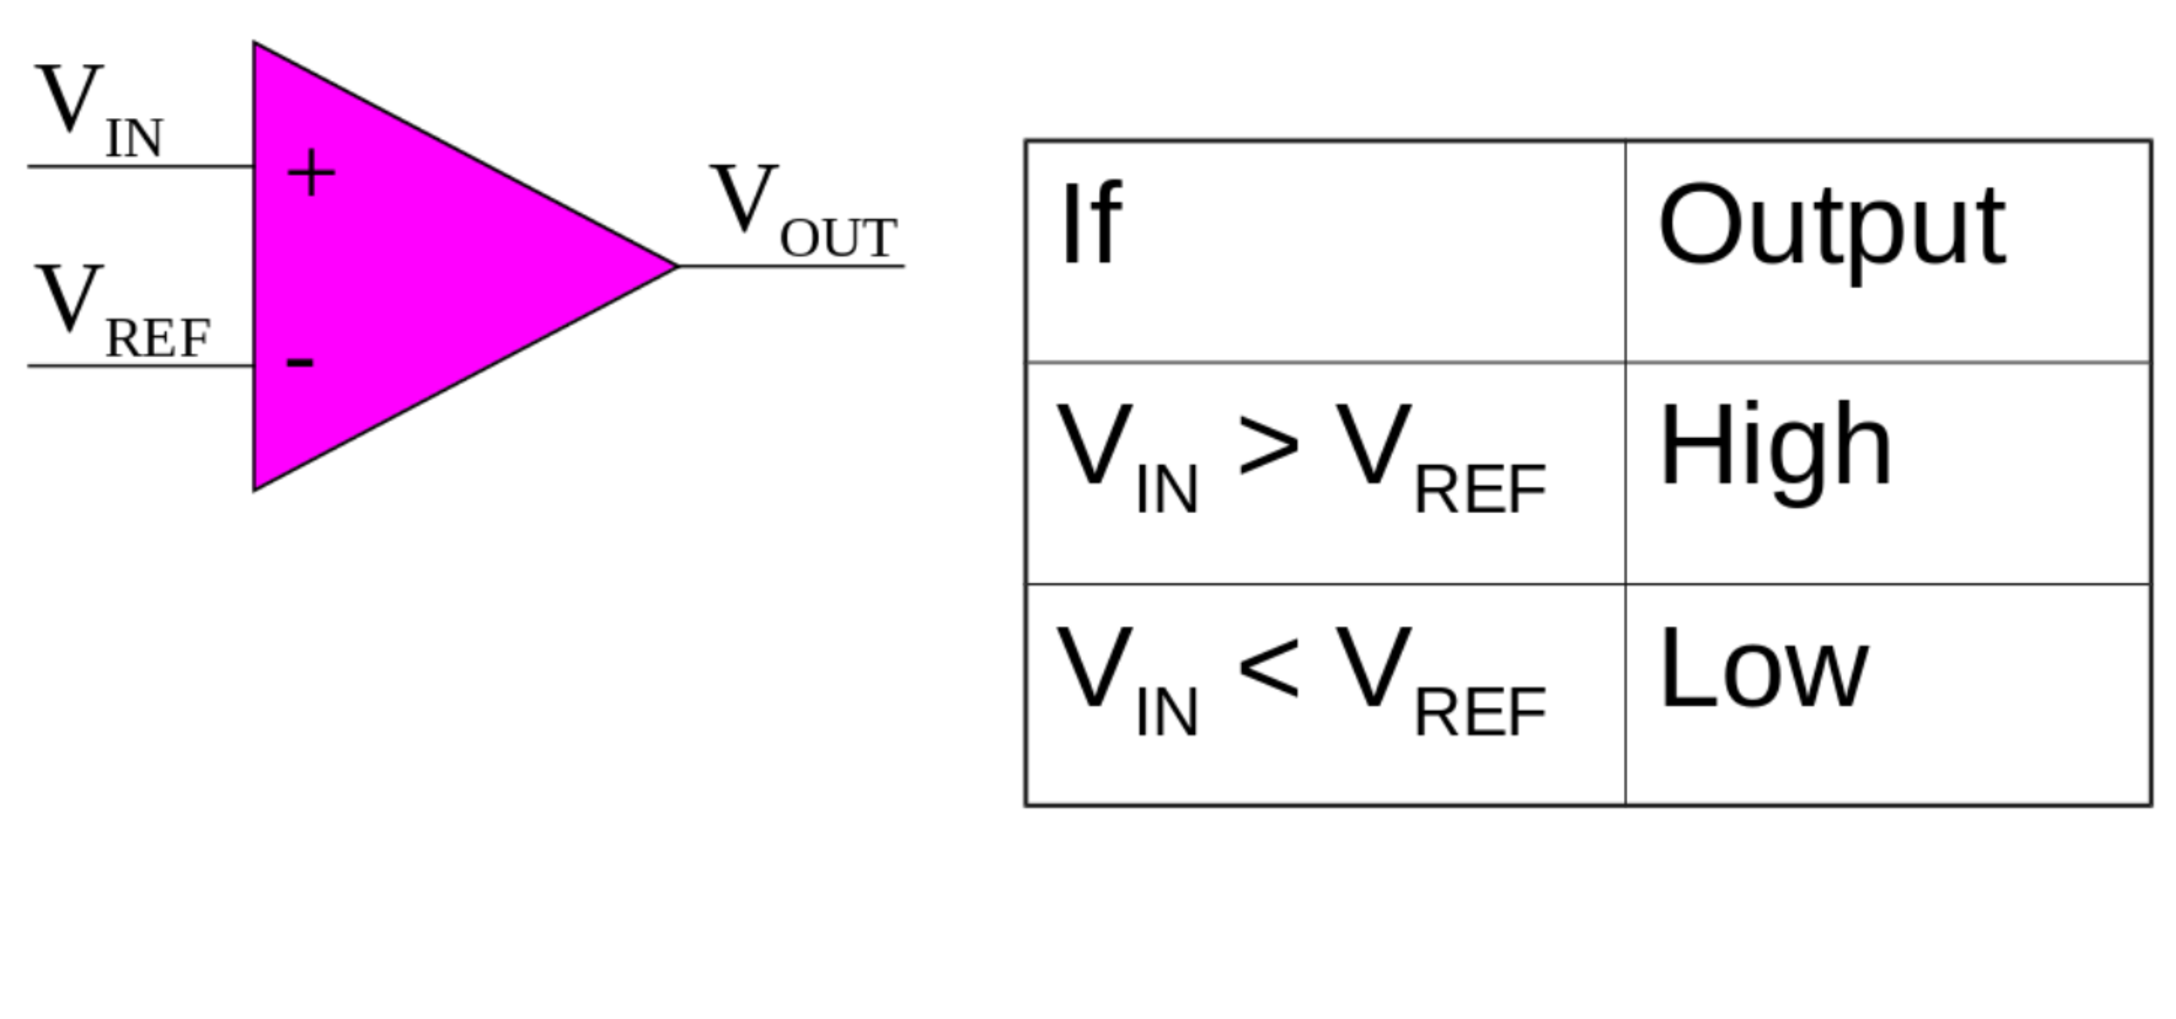
\includegraphics[height=0.35\textheight,width=0.8\textwidth]{d3/ao_comparador}
    \end{column}
  \end{columns}
  \begin{columns}
    \begin{column}{0.65\textwidth}
      \begin{block}{}
        \begin{itemize}
         \item  Utiliza una serie de comparadores
          \item  Cada comparador compara $V_{in}$ con un voltaje de referencia
distinto, comenzando por $V_{ref} = 1/2\,LSB$
        \end{itemize}
      \end{block}
    \end{column}
    \begin{column}{0.35\textwidth}
      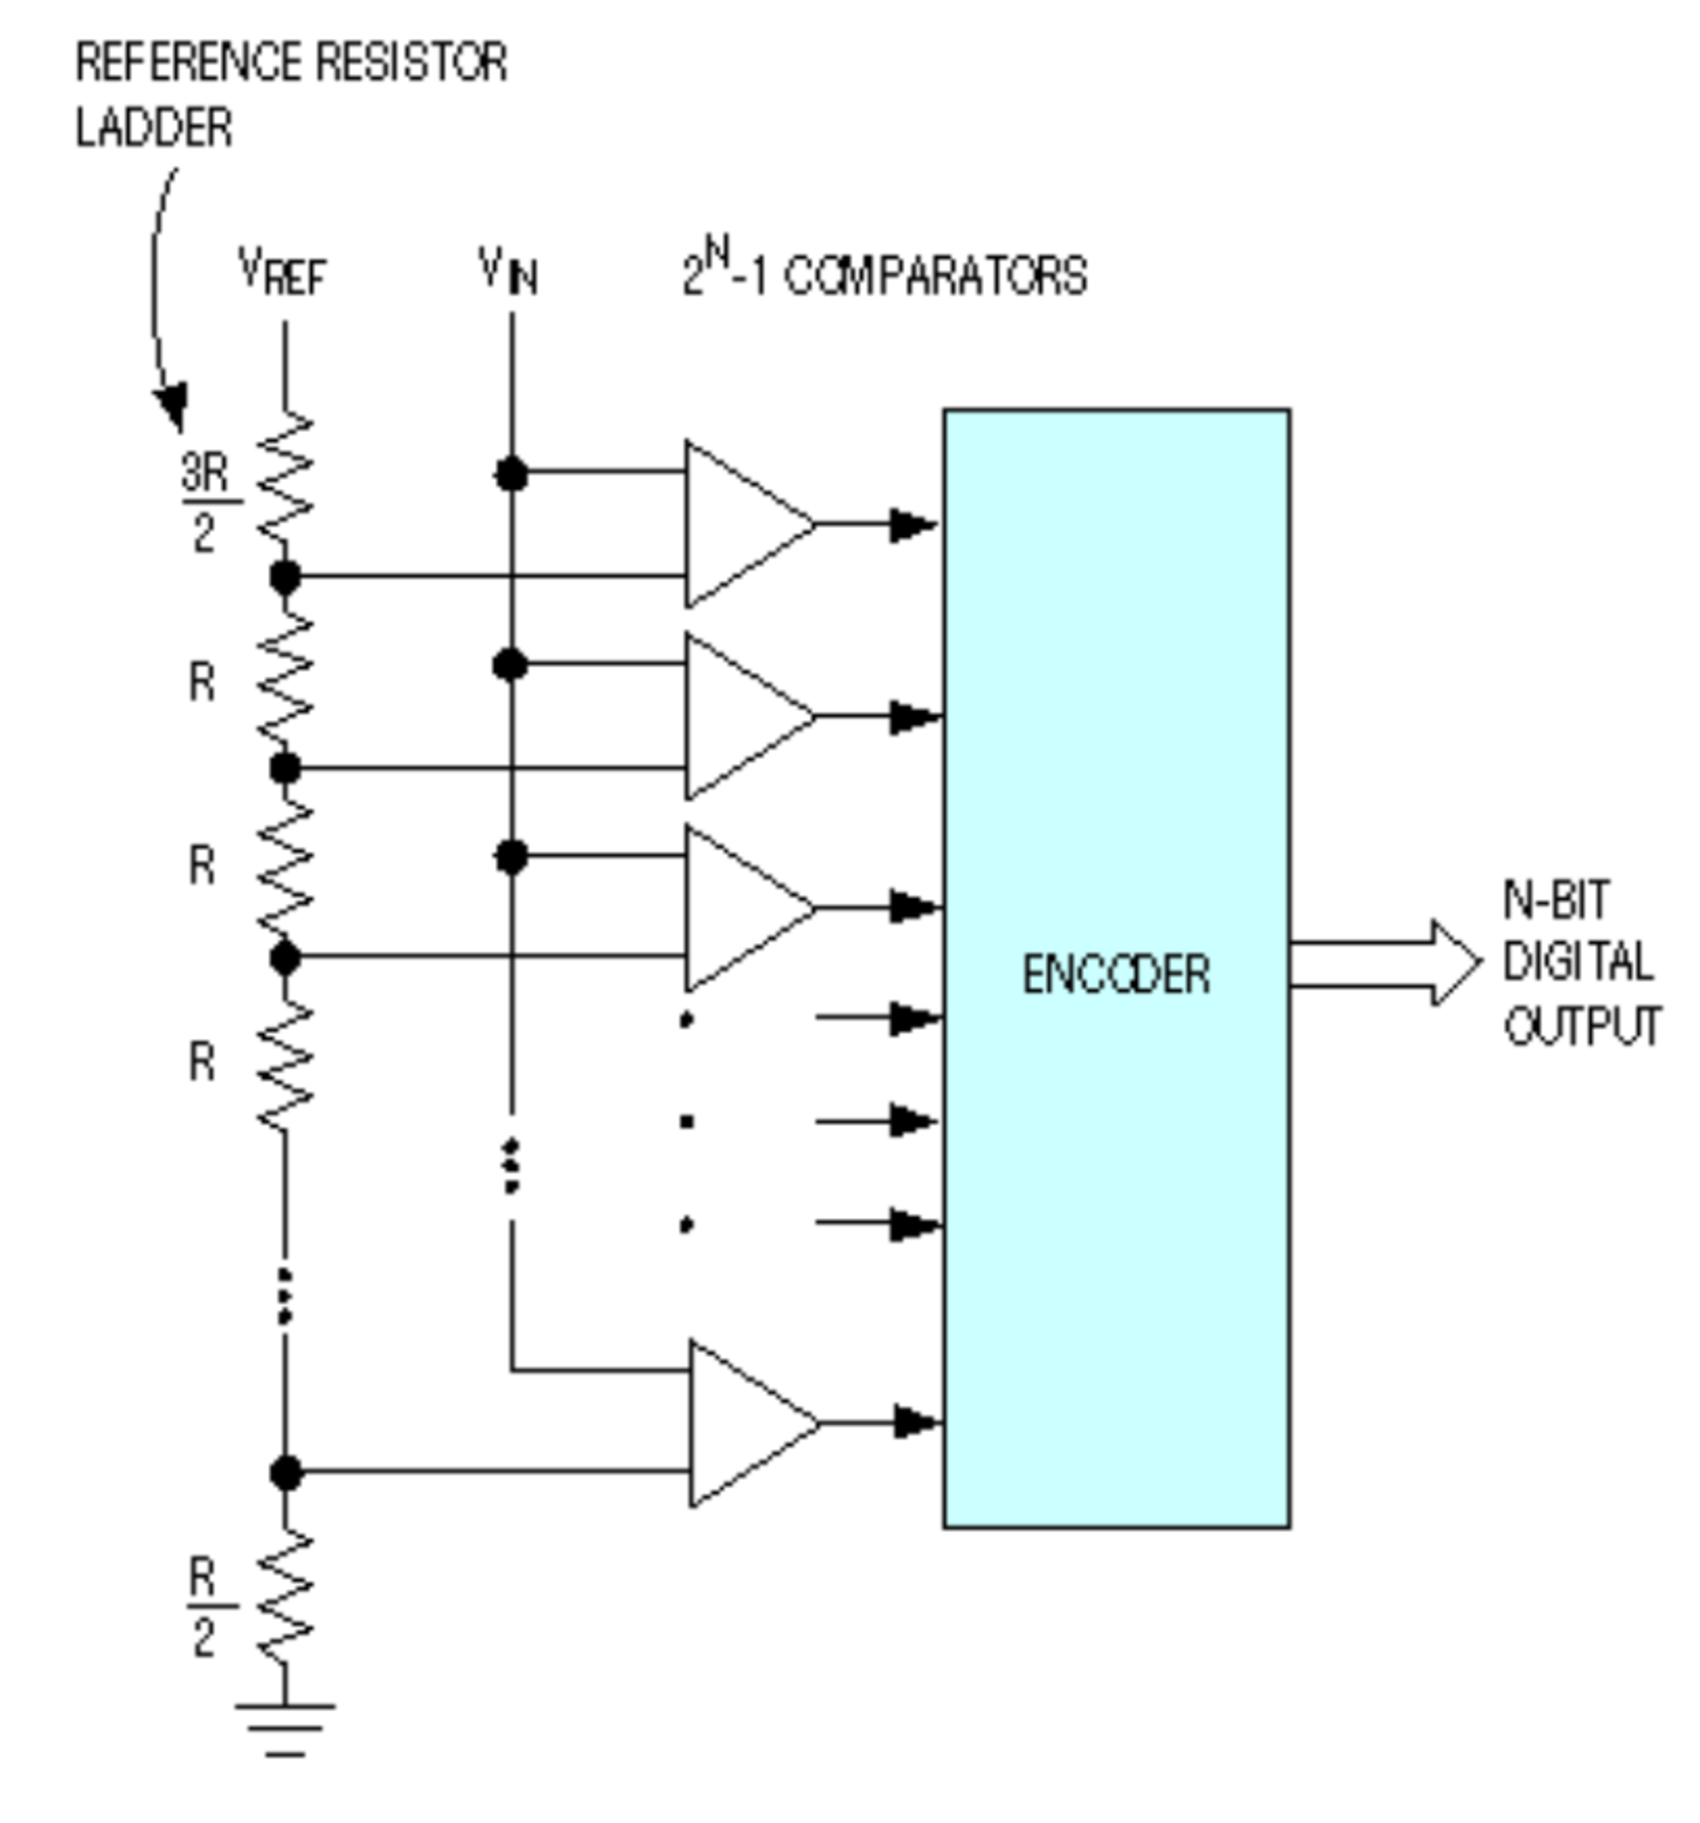
\includegraphics[height=0.45\textheight,width=0.9\textwidth]{d3/adc_flash}
    \end{column}
  \end{columns}
\end{frame}

%\begin{frame}
%\frametitle{ADC Flash}
%  \begin{columns}
%    \begin{column}{0.65\textwidth}
%      \begin{block}{}
%        \begin{itemize}
%         \item  Utiliza una serie de comparadores
%          \item  Cada comparador compara $V_{in}$ con un voltaje de referencia
%distinto, comenzando por $V_{ref} = 1/2\,LSB$
%        \end{itemize}
%      \end{block}
%    \end{column} 
%    \begin{column}{0.35\textwidth}
%      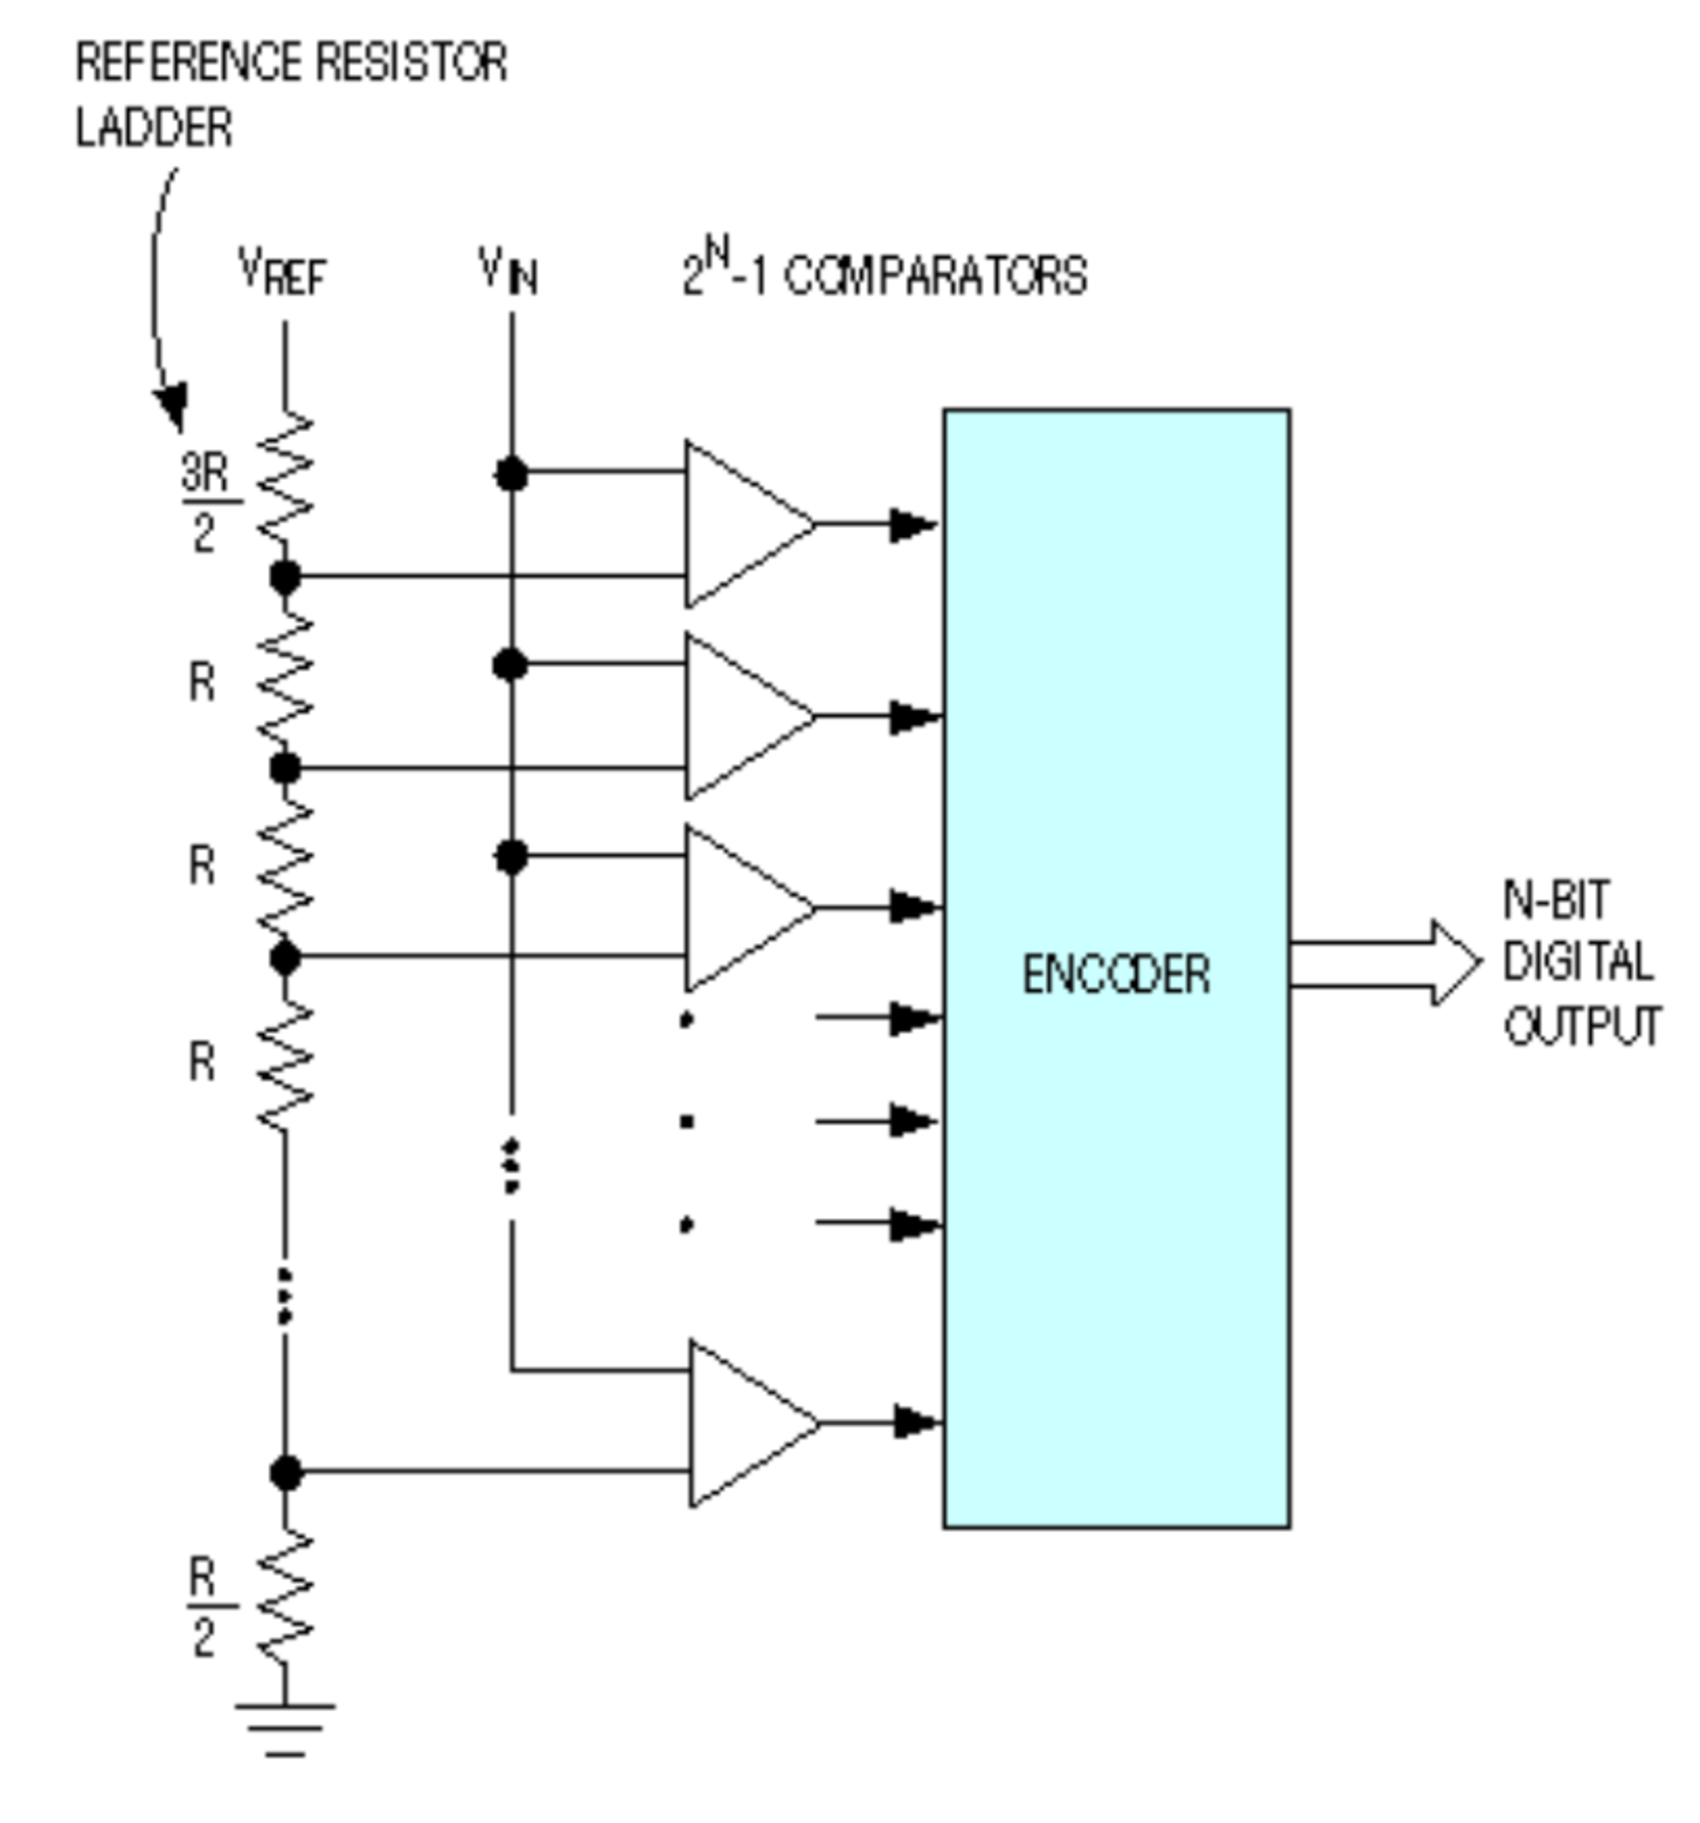
\includegraphics[height=0.5\textheight,width=0.9\textwidth]{d3/adc_flash}
%    \end{column}
%  \end{columns}
%\end{frame}

\begin{frame}
\frametitle{Ejemplos de uso}
      \begin{block}{ADC Flash}
        \begin{itemize}
          \item  Adquisición de datos (alta velocidad)
          \item  Comunicaciones satelitales
          \item  Procesamiento de señales en RADAR
          \item  Osciloscopios de muestreo
          \item  Discos rígidos de altas densidades
        \end{itemize}
      \end{block}
\end{frame}

\subsubsection{ADC de aproximaciones sucesivas}

\begin{frame}
\frametitle{ADC de aproximaciones sucesivas}
  \begin{columns}
    \begin{column}{0.6\textwidth}
        \begin{itemize}
          \item  También conocido como \textbf{SAR ADC}
(Successive-Approximation-Register ADC)
          \item  Es la arquitectura elegida en aplicaciones que requieren de
\alert{media a alta resolución}
          \item  Típicamente con frecuencias de muestreo $\leq$ {\color{blue} 5 Msps}
          \item  Buen compromiso entre velocidad y costo
        \end{itemize}
    \end{column} 
    \begin{column}{0.4\textwidth}
      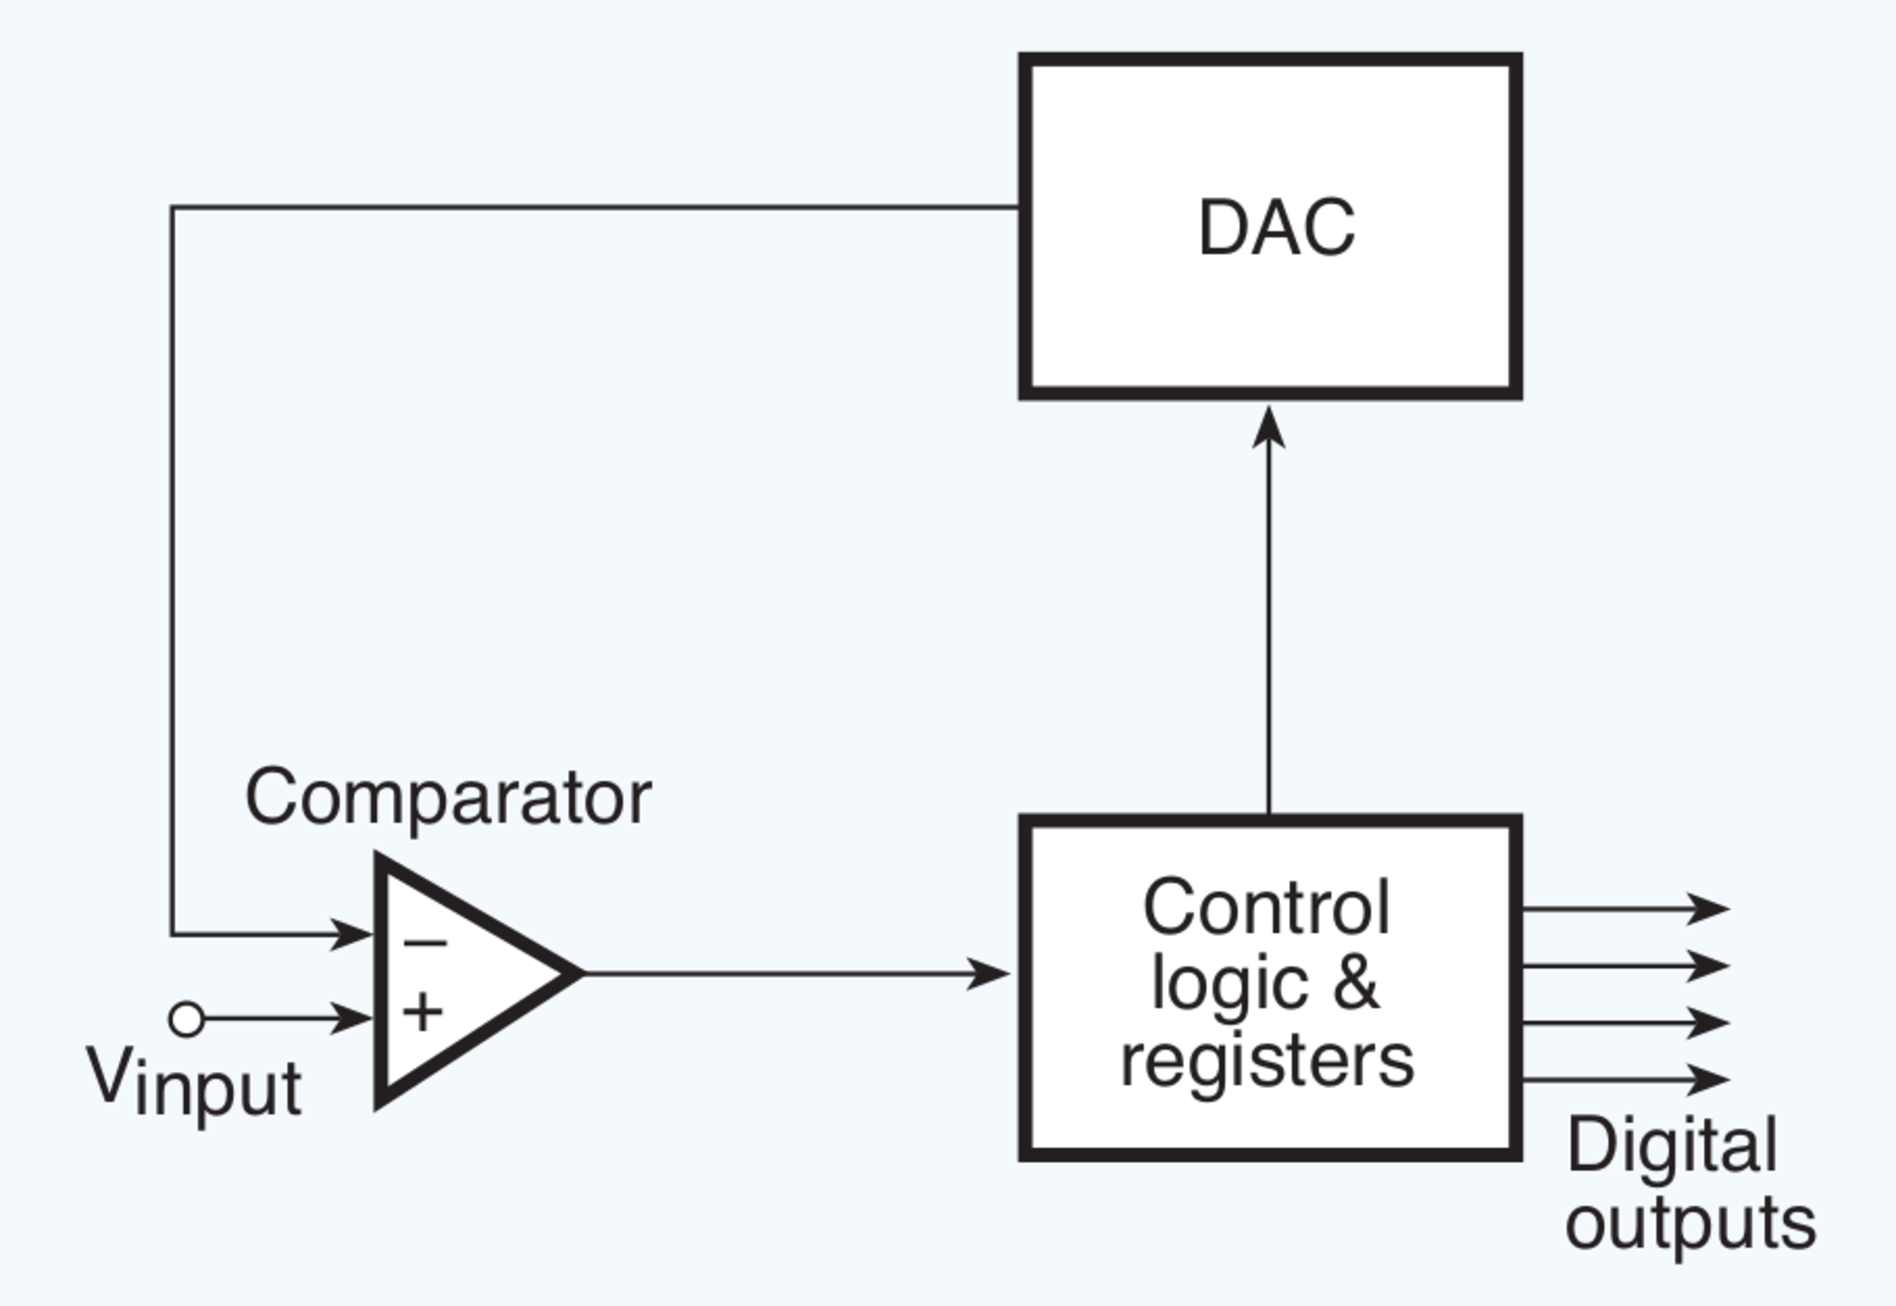
\includegraphics[width=\textwidth]{d3/adc_suc_app}
    \end{column}
  \end{columns}
\end{frame}

\begin{frame}
\frametitle{ADC de aproximaciones sucesivas}
  \begin{columns}
    \begin{column}{0.6\textwidth}
        \begin{itemize}
          \item  Se los encuentra principalmente con resoluciones que van de
{\color{blue} 8 a 16 bits}
          \item  Relativamente poco consumo de potencia
          \item  Pequeño factor de forma (prestaciones vs. tamaño)%FIXME: explicar qué es el factor de
%forma
        \end{itemize}
    \end{column} 
    \begin{column}{0.4\textwidth}
      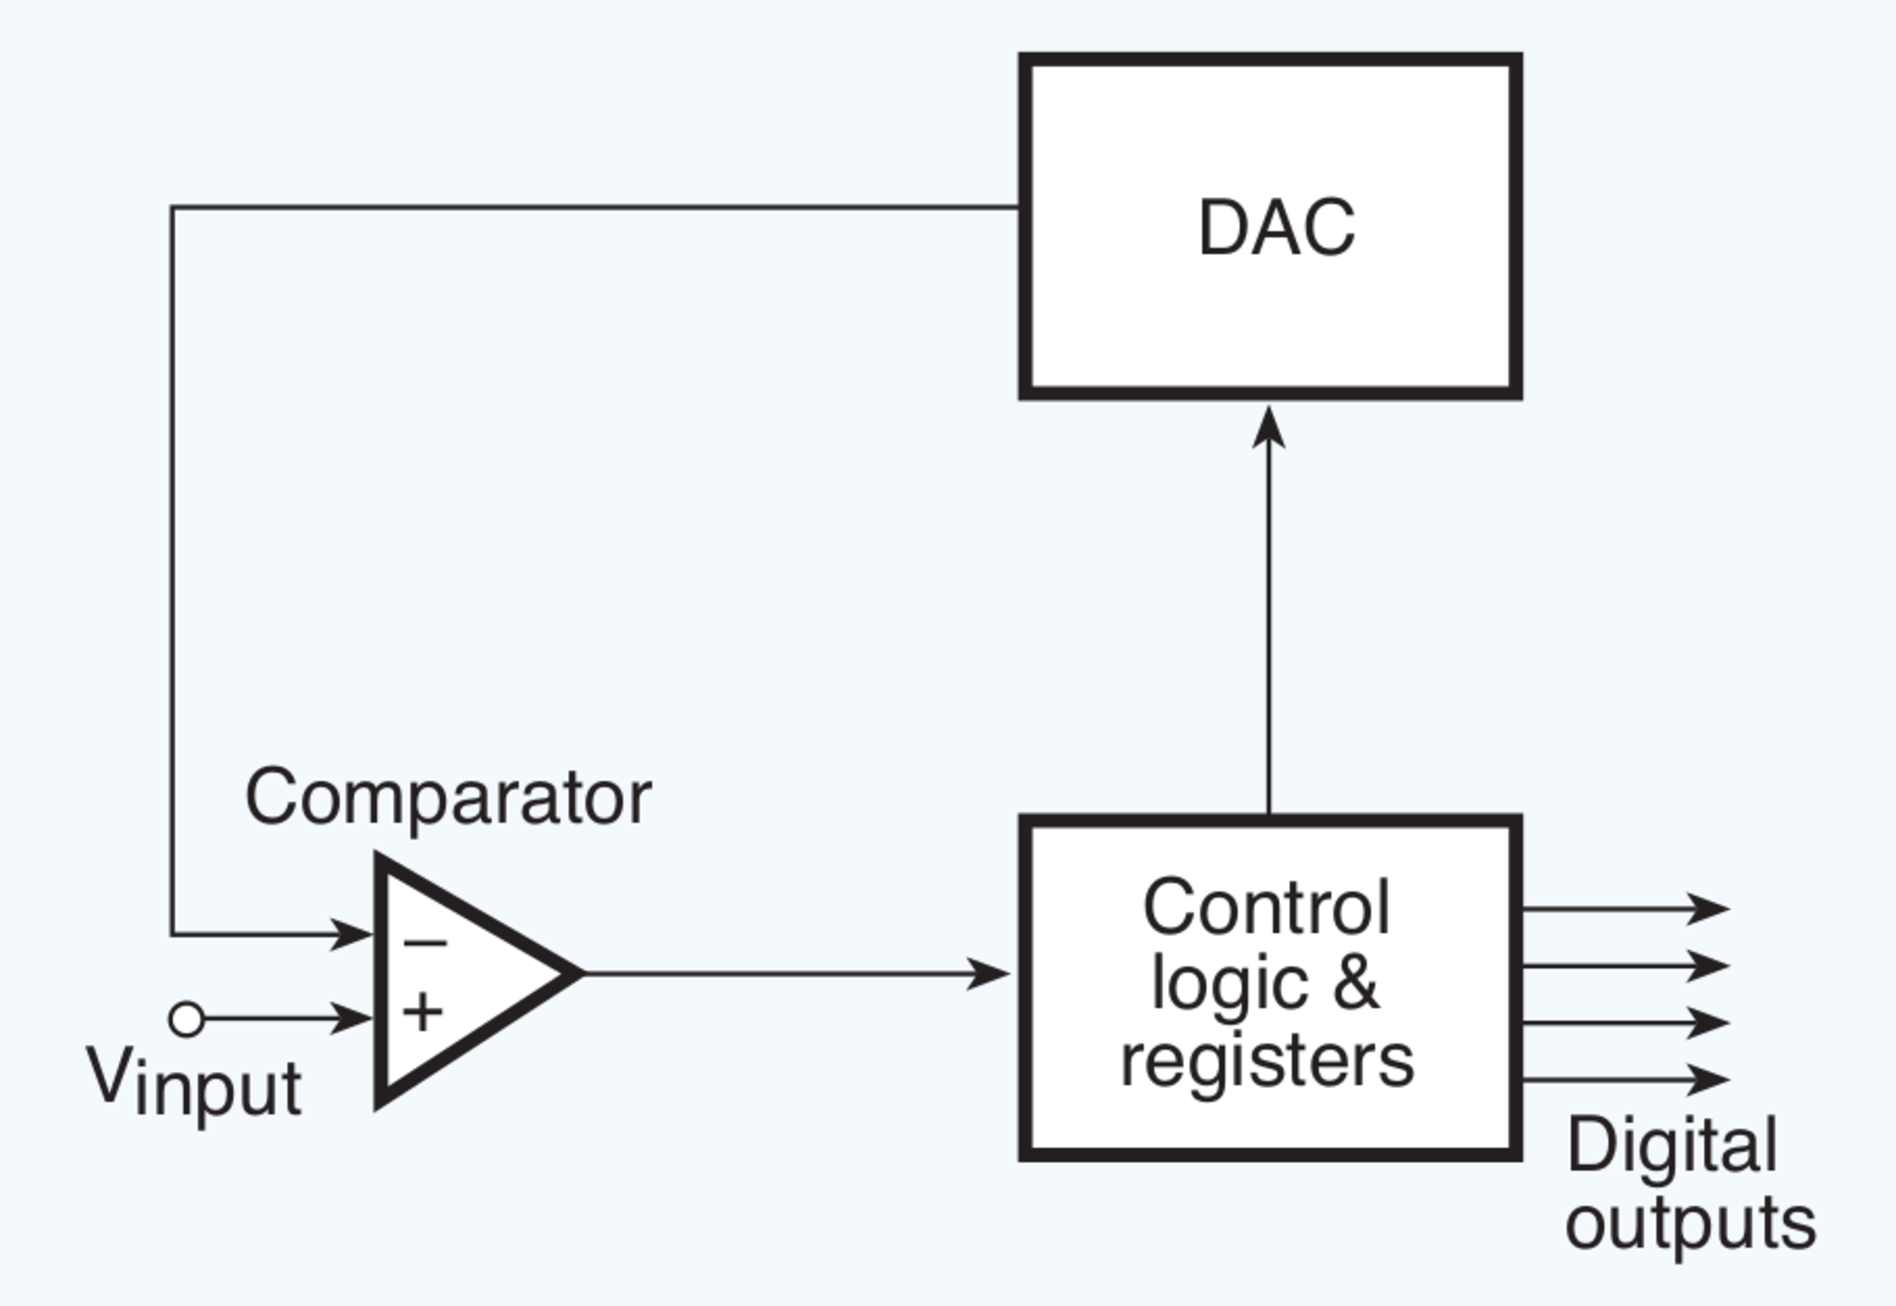
\includegraphics[width=\textwidth]{d3/adc_suc_app}
    \end{column}
  \end{columns}
\end{frame}

\begin{frame}
\frametitle{Algoritmo de comparación}
\begin{columns}
    \begin{column}{0.65\textwidth}
      \begin{exampleblock}{}
        \begin{enumerate}
          \item Coloca el MSB a mitad de escala 
          \item Convierte el MSB a analógico usando el DAC 
          \item Compara la estimación con la entrada 
          \item Coloca el bit correspondiente
          \item Verifica el bit siguiente
        \end{enumerate}
      \end{exampleblock}
    \end{column} 
    \begin{column}{0.35\textwidth}
      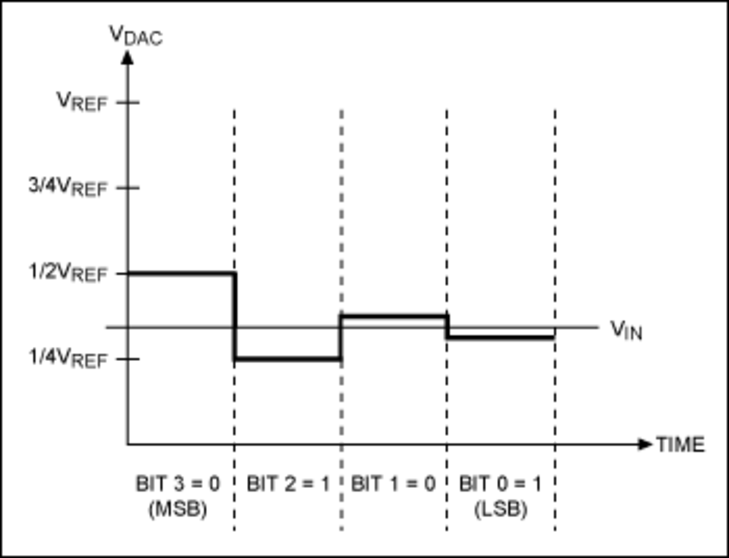
\includegraphics[width=\textwidth]{d3/sar_adc}
    \end{column} 
  \end{columns}
      \begin{exampleblock}{Ejemplos de uso}
        \begin{itemize}
          \item  Instrumentación portable, alimentada con baterías
          \item  Controles industriales
          \item  Adquisición de datos/señales
          \item  Bolígrafos digitalizadores 
        \end{itemize}
      \end{exampleblock}
\end{frame}

%\begin{frame}
%\frametitle{Ejemplos de uso}
%  \begin{columns}
%    \begin{column}{0.45\textwidth}
%      \begin{block}{}
%        \begin{itemize}
%          \item  Instrumentación portable, alimentada con baterías
%          \item  Controles industriales
%          \item  Adquisición de datos/señales
%          \item  Bolígrafos digitalizadores 
%        \end{itemize}
%      \end{block}
%    \end{column} 
%  \end{columns}
%\end{frame}

\subsubsection{ADC conversor de voltaje a frecuencia}

\begin{frame}
\frametitle{ADC conversor de voltaje a frecuencia}
  \begin{columns}
    \begin{column}{0.65\textwidth}
        \begin{itemize}
          \item {\color{blue} Convierte $V_{in}$ en un tren de pulsos cuya
frecuencia es proporcional a la amplitud de la entrada}
          \item Cuenta pulsos durante {\color{blue}un período fijo} para determinar la
frecuencia, y la salida del contador, a su vez, representa el voltaje digital
          \item \alert{Característica de rechazo de ruido elevada}, porque la
señal de entrada se integra eficazmente durante el intervalo de conteo 
        \end{itemize}
    \end{column} 
    \begin{column}{0.35\textwidth}
      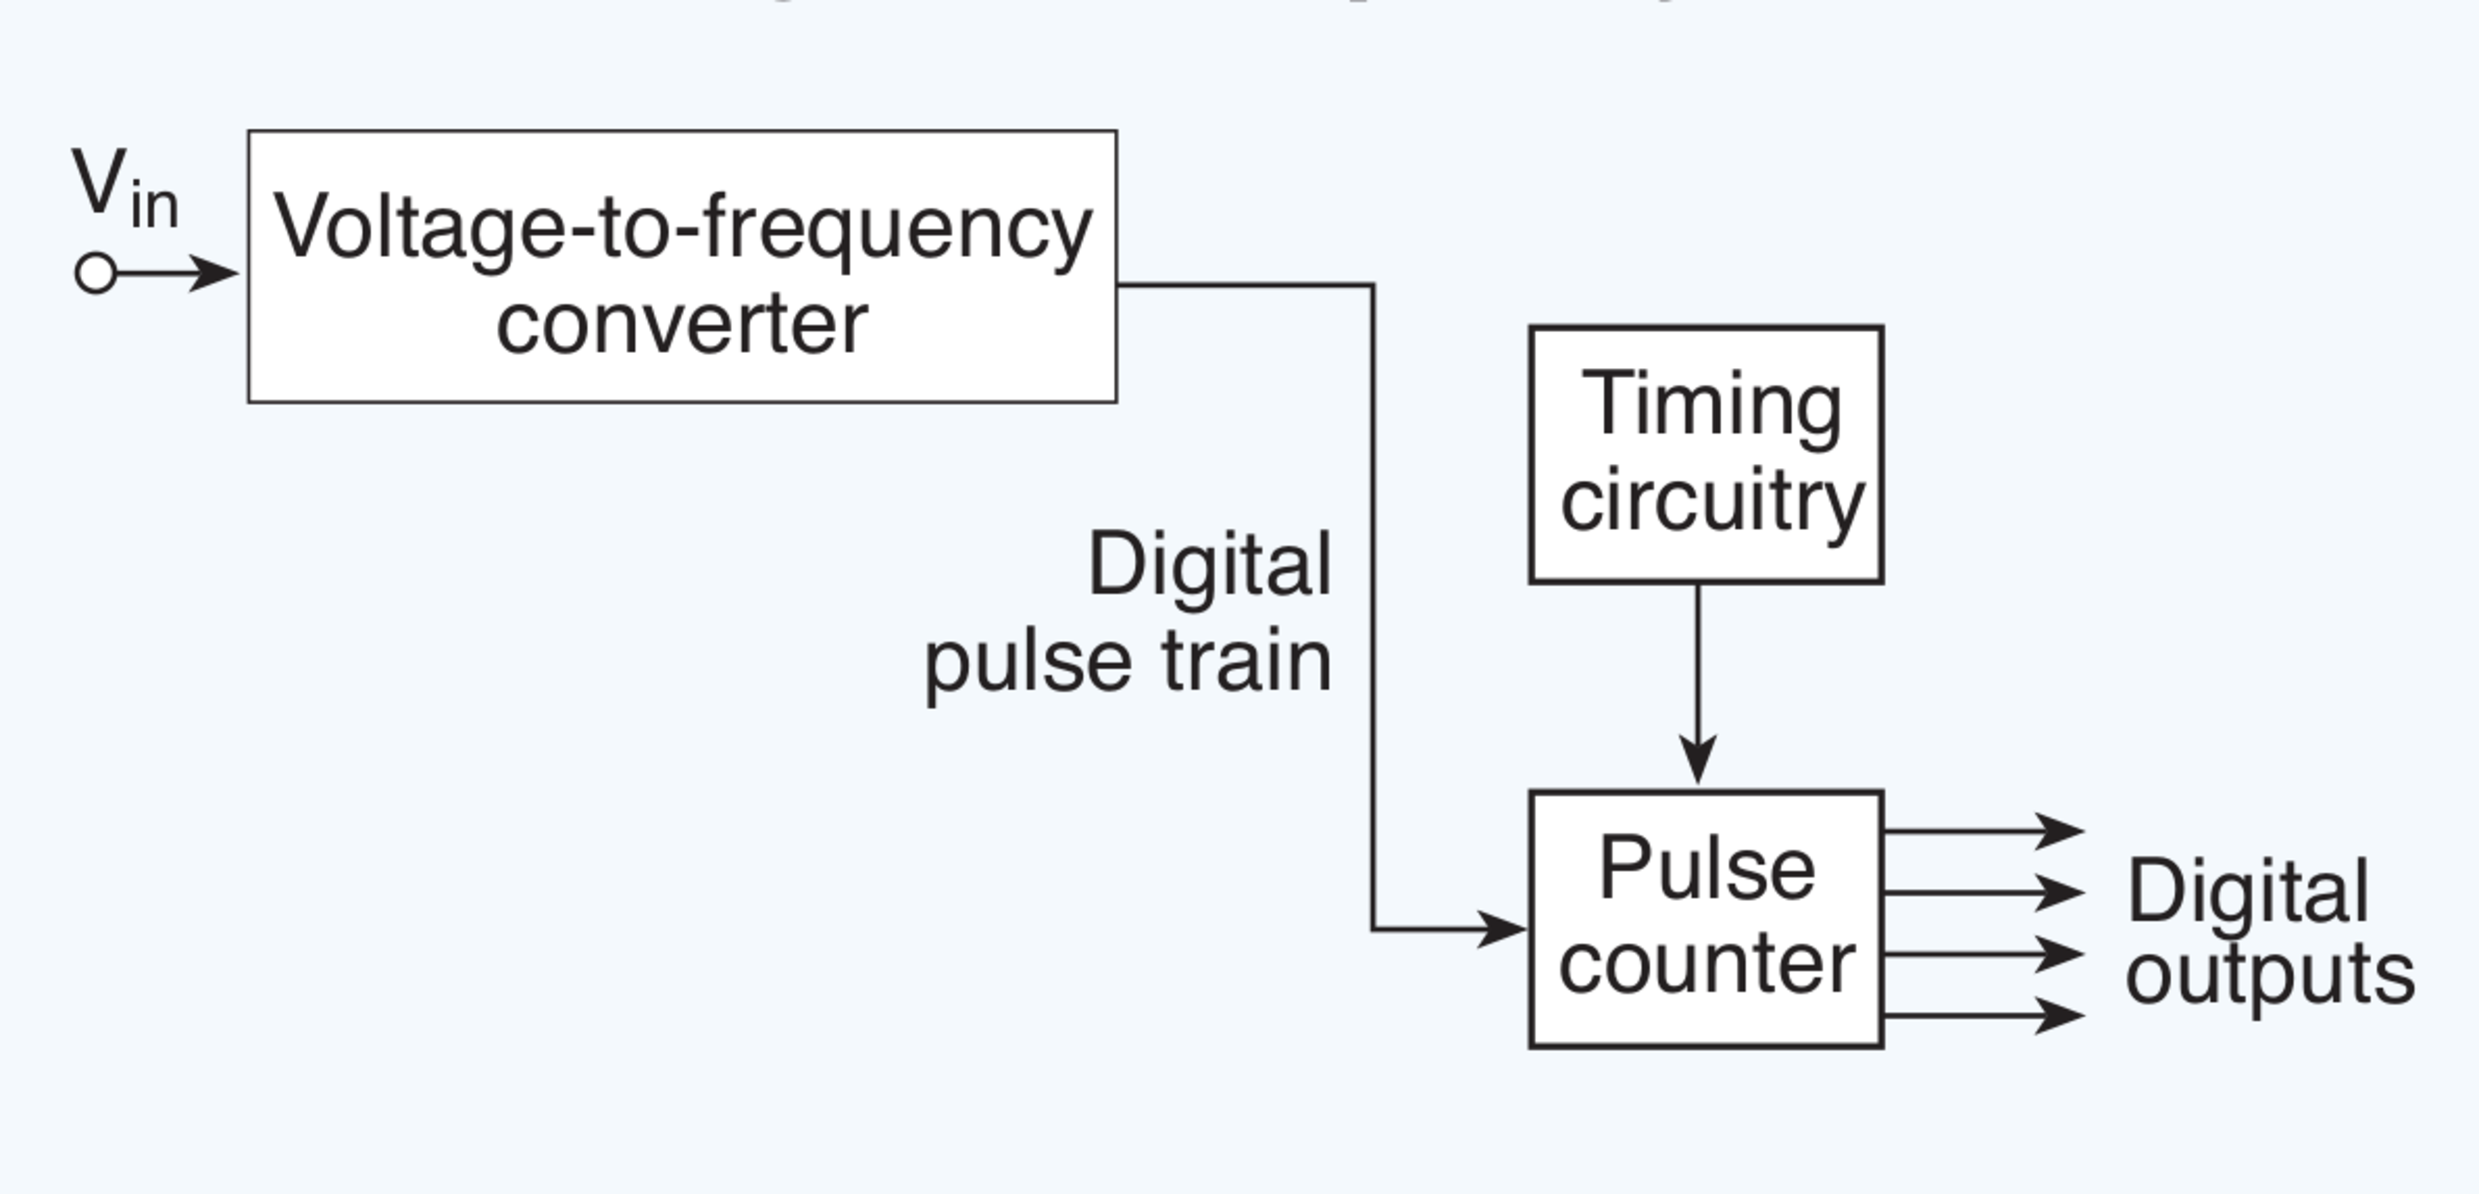
\includegraphics[width=\textwidth]{d3/adc_v_to_f}
    \end{column}
  \end{columns}
      \begin{alertblock}{Ejemplos de uso}
        \begin{itemize}
          \item Comúnmente usados para convertir señales lentas y ruidosas 
          \item Aplicaciones remotas en ambientes ruidosos   
        \end{itemize}
      \end{alertblock}
\end{frame}

\subsubsection{ADC de doble envolvente}

\begin{frame}
\frametitle{ADC de doble envolvente}
  \begin{columns}
    \begin{column}{0.6\textwidth}
     % \begin{block}{}
        \begin{itemize}
          \item Carga un condensador durante un período fijo $\rightarrow$
\alert{corriente proporcional a la tensión de entrada}
\item Entonces, el tiempo requerido para descargar el mismo condensador bajo una
\alert{corriente constante} determina el valor de $V_{in}$
        \end{itemize}
      %\end{block}
    \end{column} 
    \begin{column}{0.4\textwidth}
      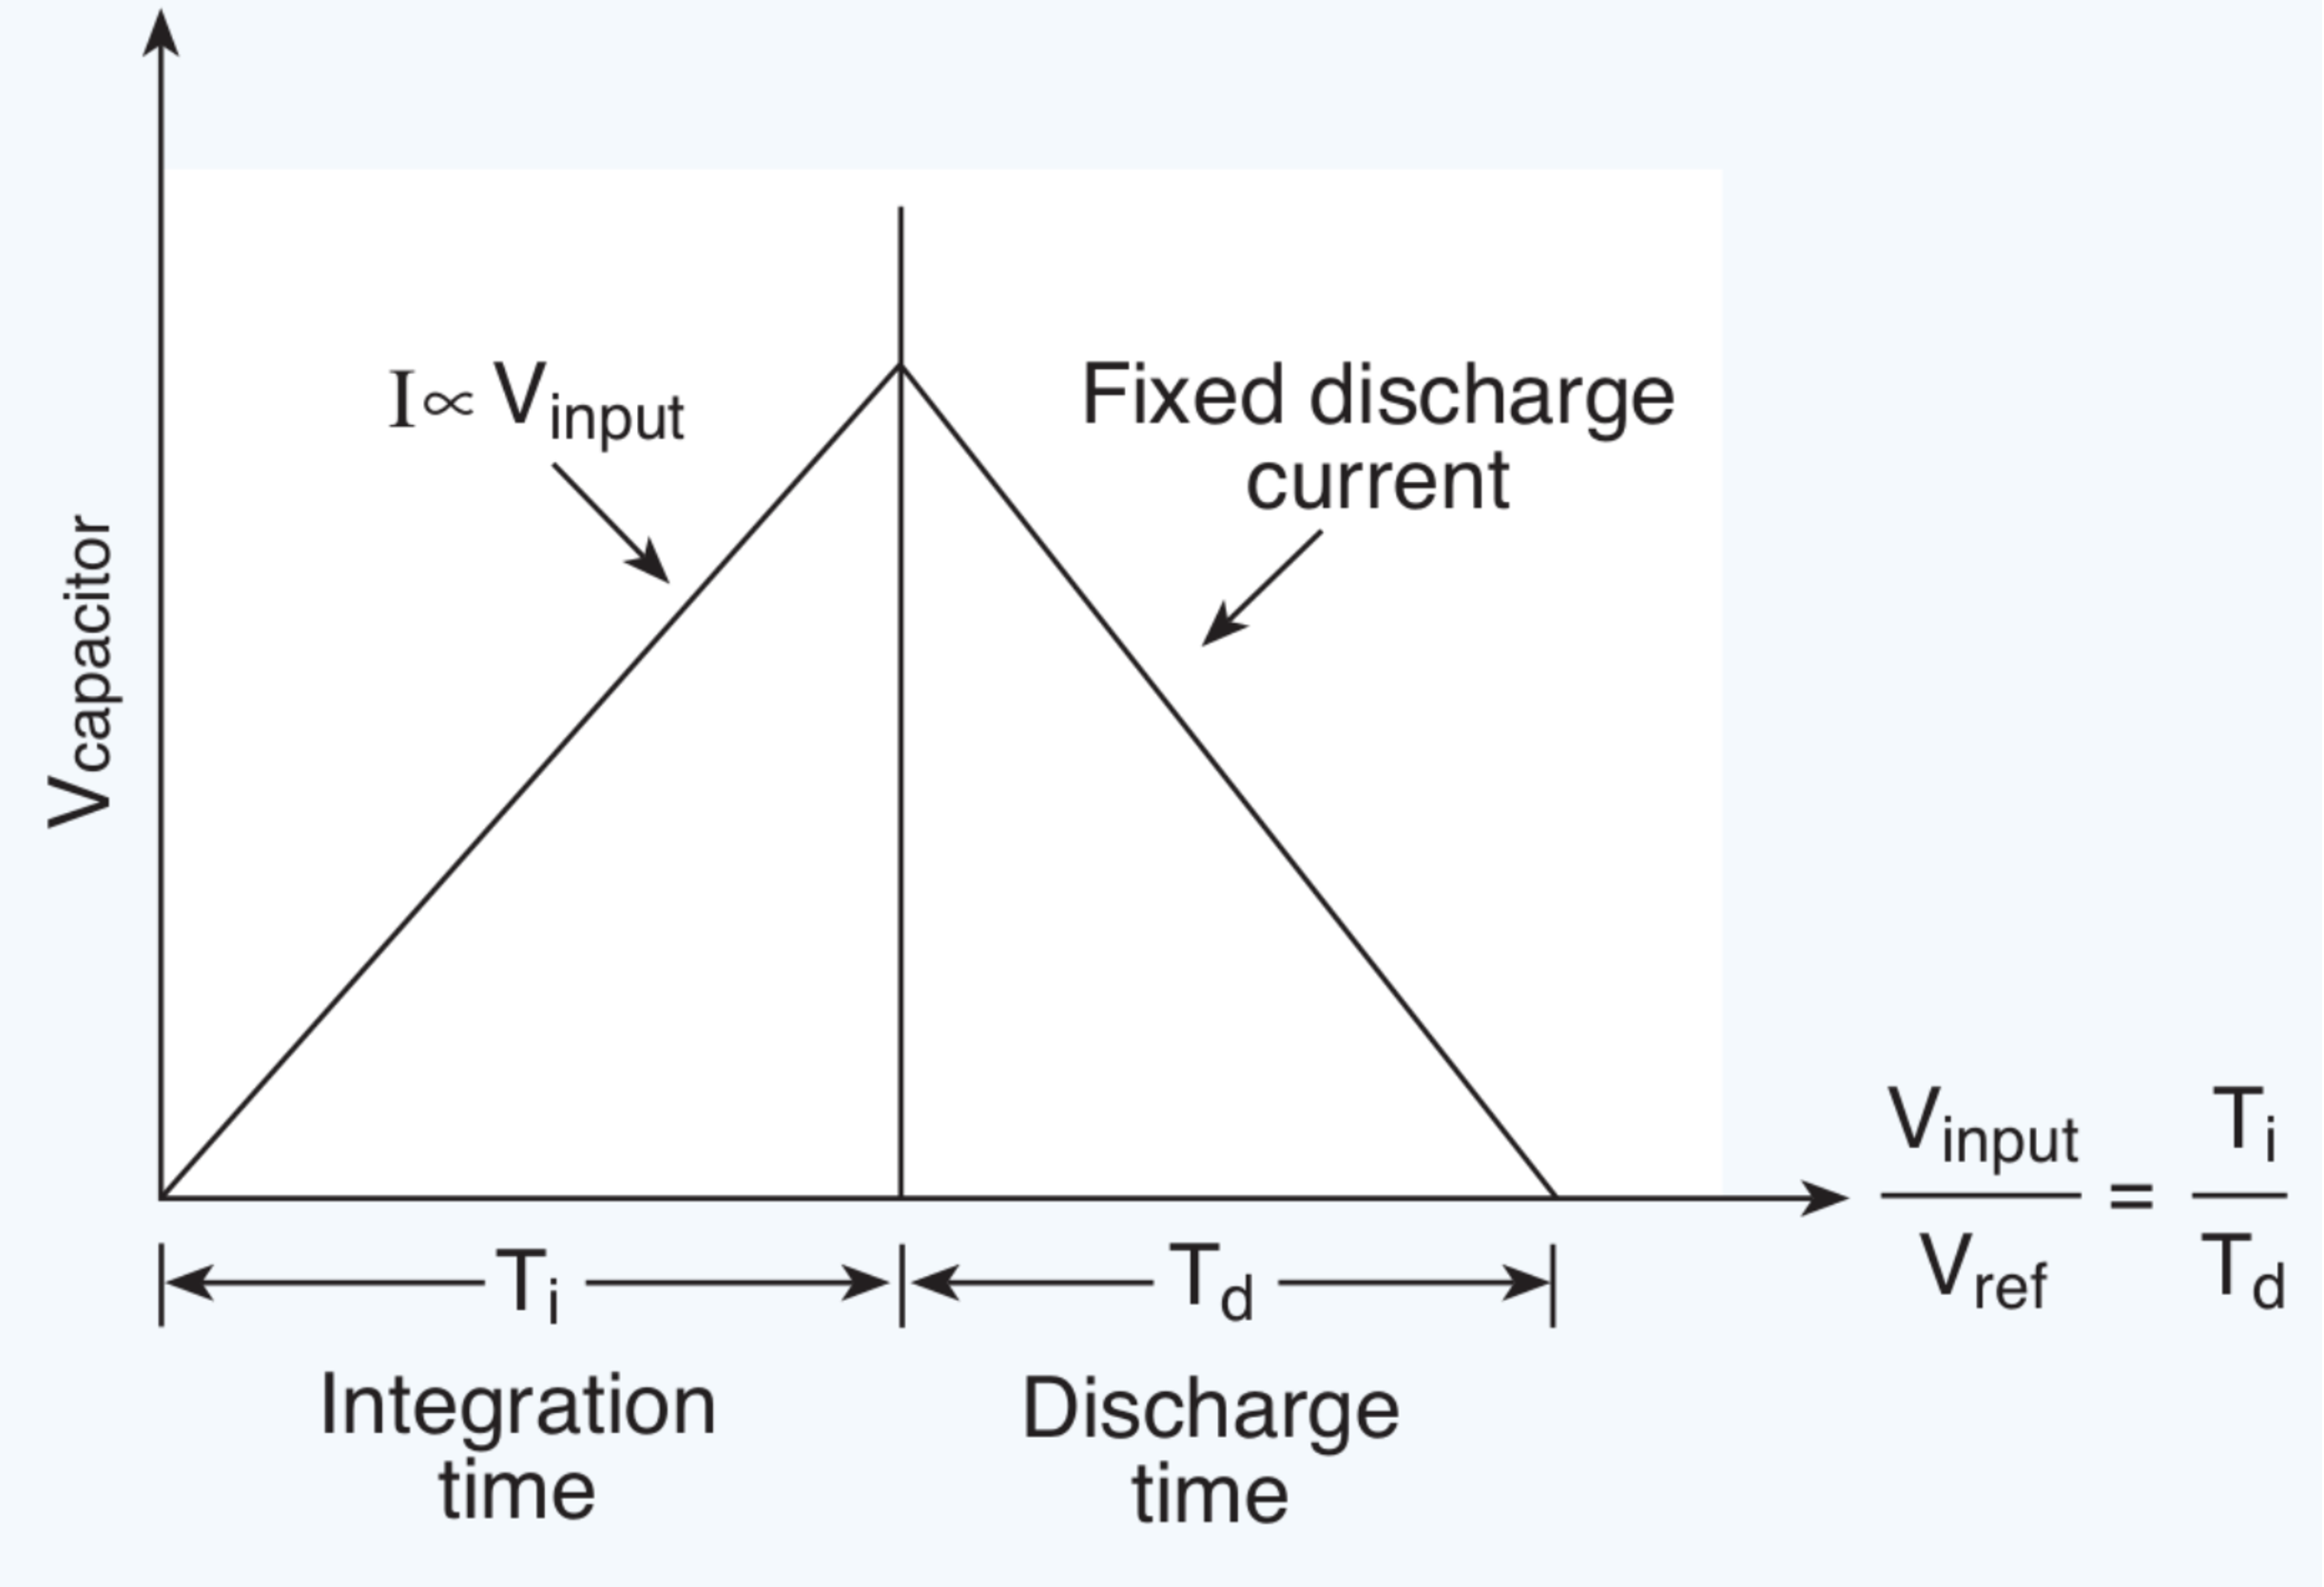
\includegraphics[width=\textwidth]{d3/adc_dual_slope_curve}
    \end{column}
  \end{columns}
      \begin{block}{}
{\color{blue} La técnica es relativamente precisa y estable porque
depende de la relación entre el tiempo de subida y el tiempo de caída, no sobre
el valor absoluto del condensador u otros componentes cuyos valores cambian con
el tiempo, temperatura, etc.}  
      \end{block}
\end{frame}

\begin{frame}
\frametitle{ADC de doble envolvente}
\begin{columns}
\begin{column}{0.4\textwidth}
      %\begin{alertblock}{}
\begin{center}     
      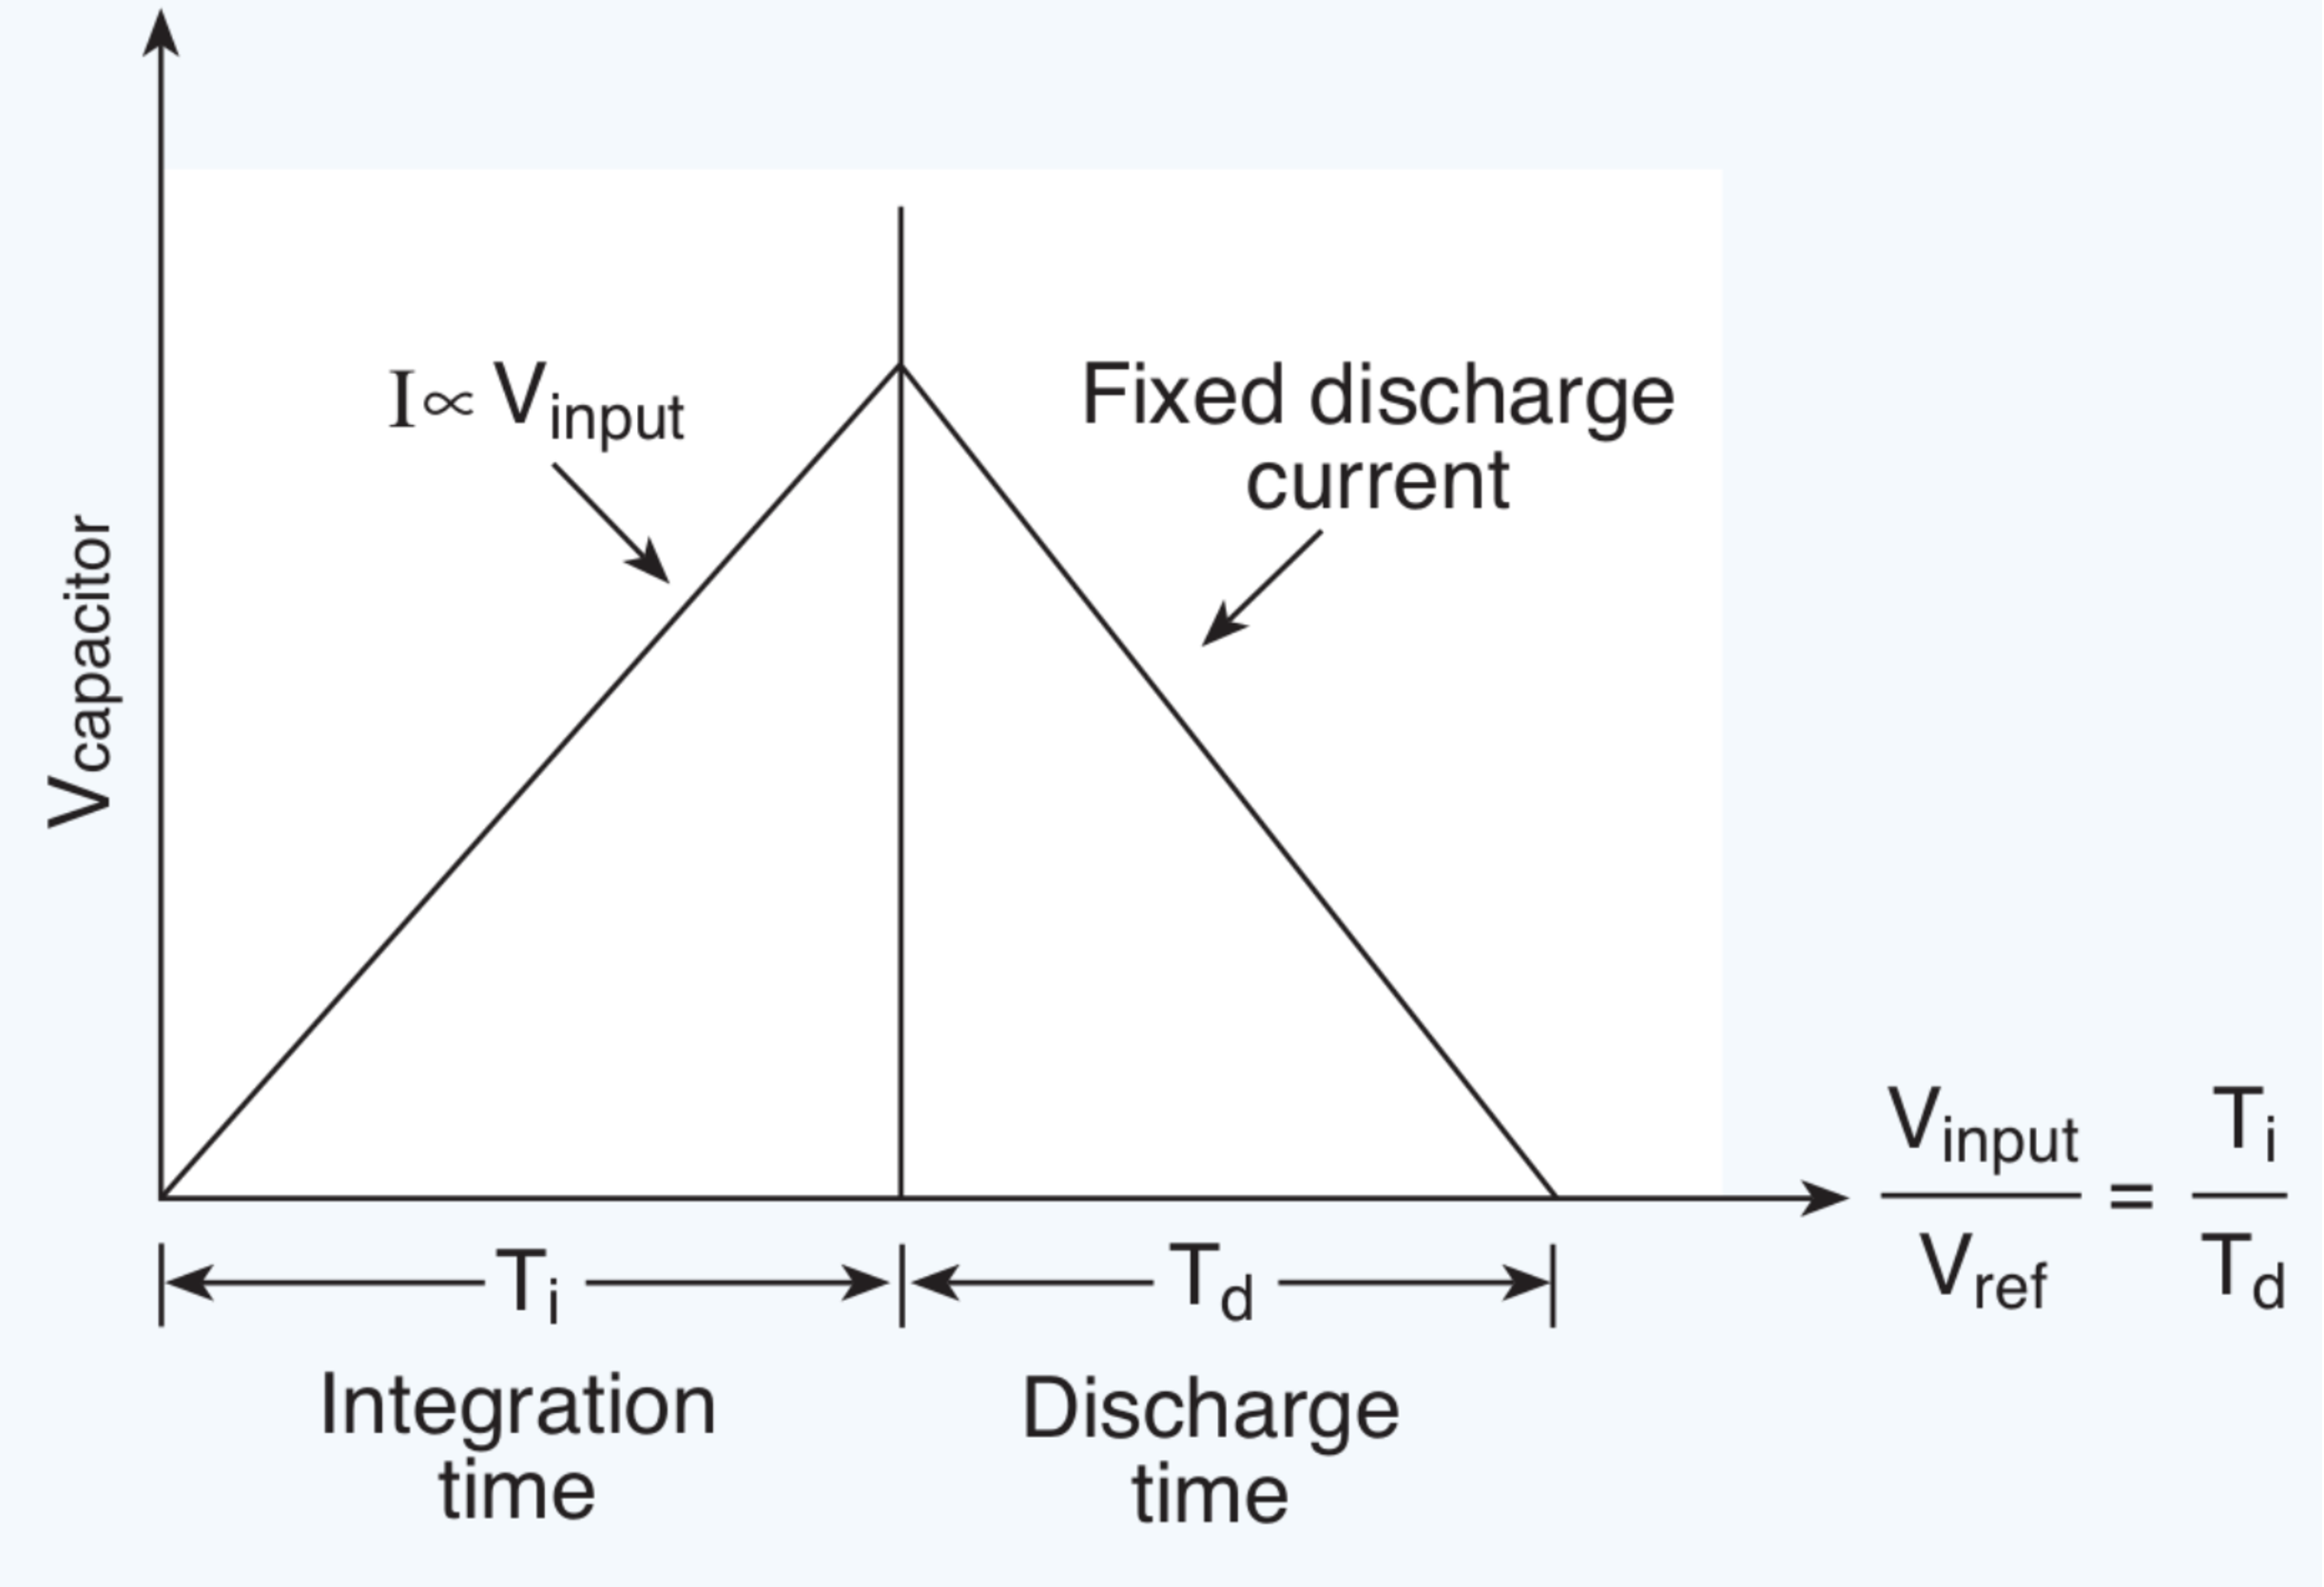
\includegraphics[height=0.4\textheight,width=\textwidth]{d3/adc_dual_slope_curve}
\end{center}     
      %\end{alertblock}
\end{column}
\begin{column}{0.6\textwidth}
\begin{alertblock}{Usos}
\begin{itemize}
\item La integración de $V_{in}$ reduce la captación de ruido en la frecuencia
de línea de CA cuando el tiempo de integración coincide con un múltiplo del periodo
\item {\color{blue} Se utiliza a menudo en multímetros digitales de precisión y
medidores de panel}
\item Aunque la precisión de 20 bits es común, tiene una tasa de conversión relativamente 
lenta
\end{itemize}
\end{alertblock}
\end{column}
\end{columns}
\end{frame}

\subsubsection{ADC Sigma-Delta}

\begin{frame}
\frametitle{ADC Sigma-Delta}
\begin{exampleblock}{}
  \begin{center}
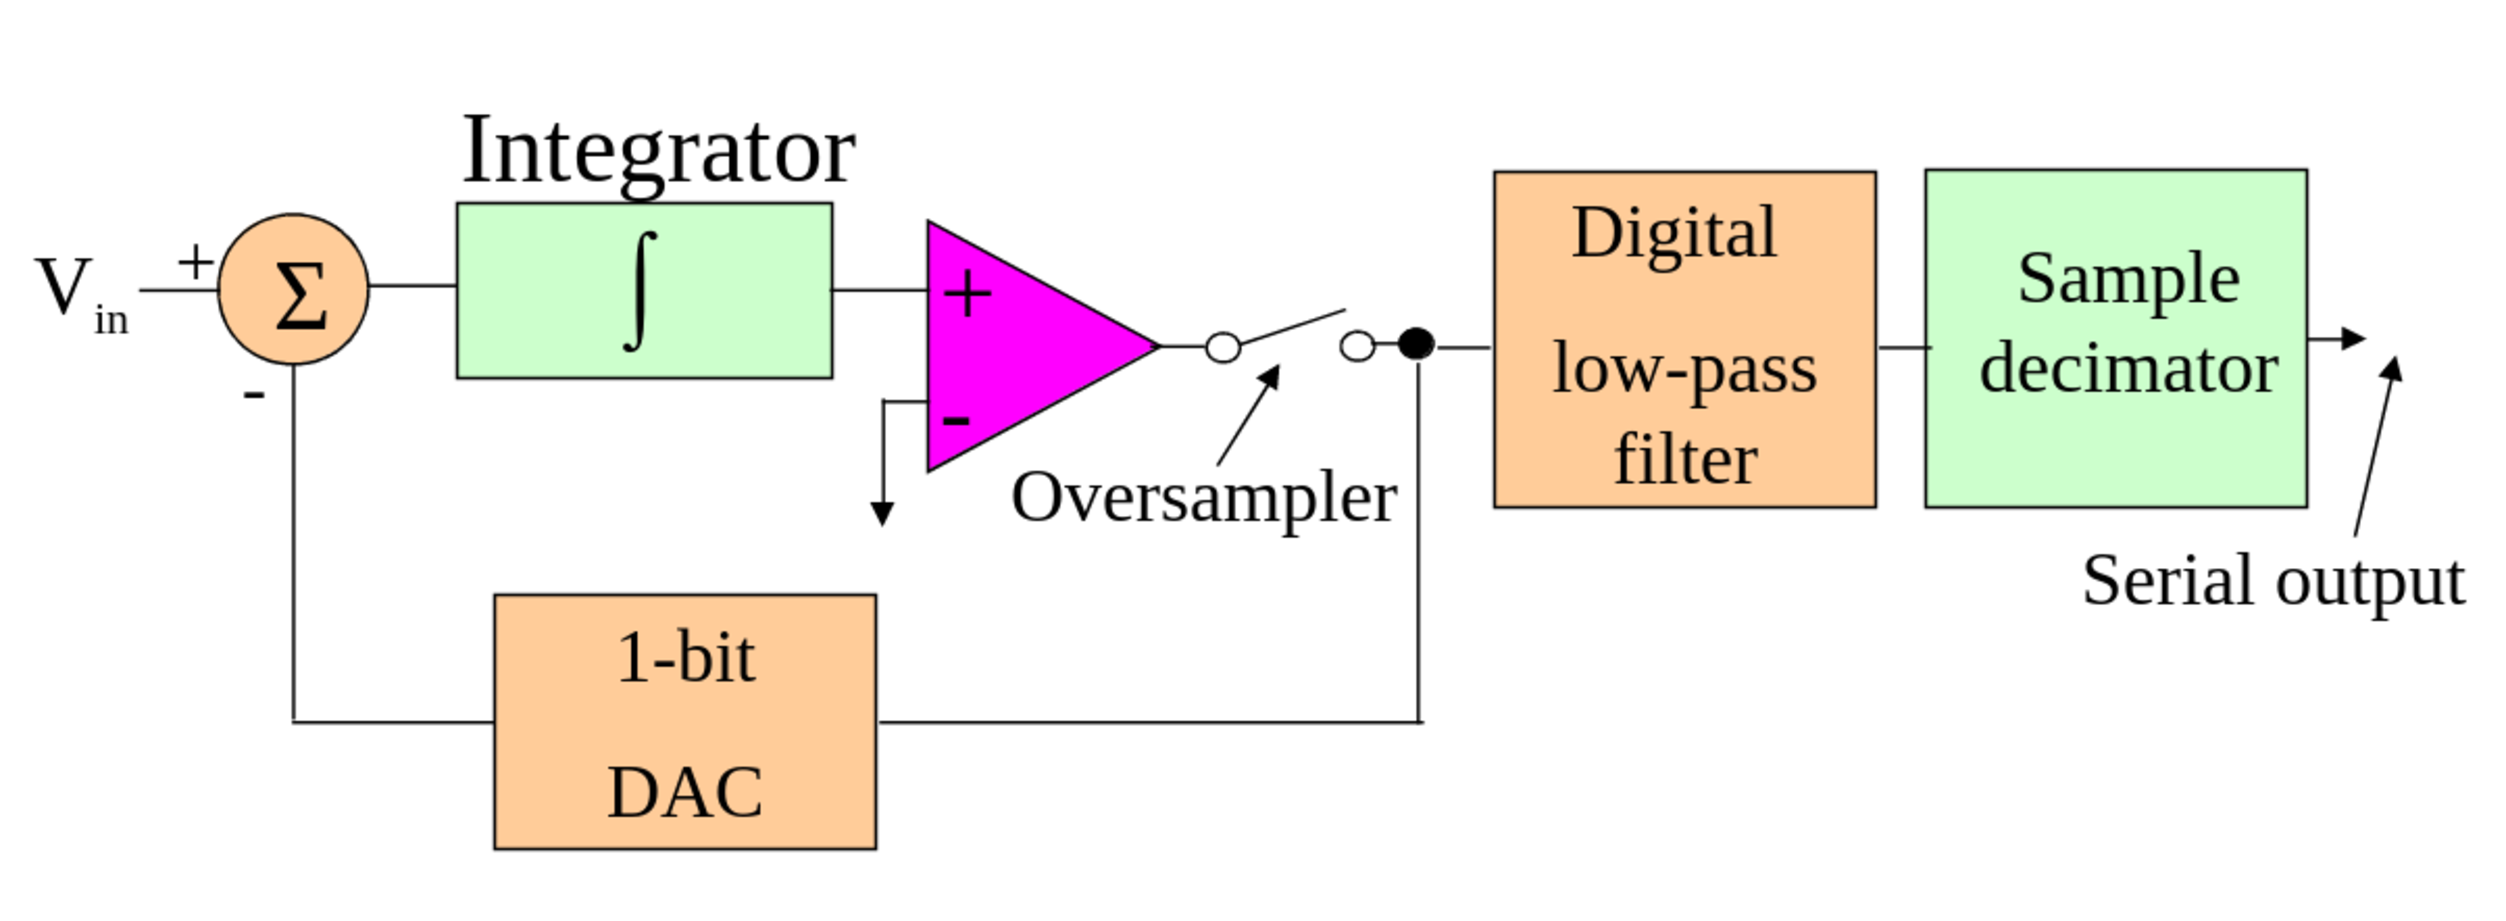
\includegraphics[width=0.8\textwidth]{d3/sigma_delta_adc}
  \end{center}
\end{exampleblock}
\begin{exampleblock}{}
        \begin{itemize}
          \item Itera para producir una serie de bits
          \item La salida es una serie de bits con el número de 1's proporcional a $V_{in}$
          \item El DAC mantiene la salida del integrador cerca del nivel de
tensión de referencia
        \end{itemize}
\end{exampleblock}
\end{frame}

\begin{frame}
\frametitle{ADC Sigma-Delta}
  \begin{columns}
    \begin{column}{0.55\textwidth}
      \begin{exampleblock}{}
        \begin{itemize}
          \item  Utilizados predominantemente en aplicaciones de baja velocidad,
donde se requiere un compromiso entre velocidad para oversampling, seguido de
filtrado para reducir el ruido
          \item  Son comunes los conversores de 24 bits para aplicaciones de
audio, instrumentación y sonar
          \item  Los anchos de banda son típicamente menores a $1\,MHz$, con un
rango de 12 a 18 bits verdaderos
        \end{itemize}
      \end{exampleblock}
    \end{column} 
    \begin{column}{0.45\textwidth}
  \begin{center}
      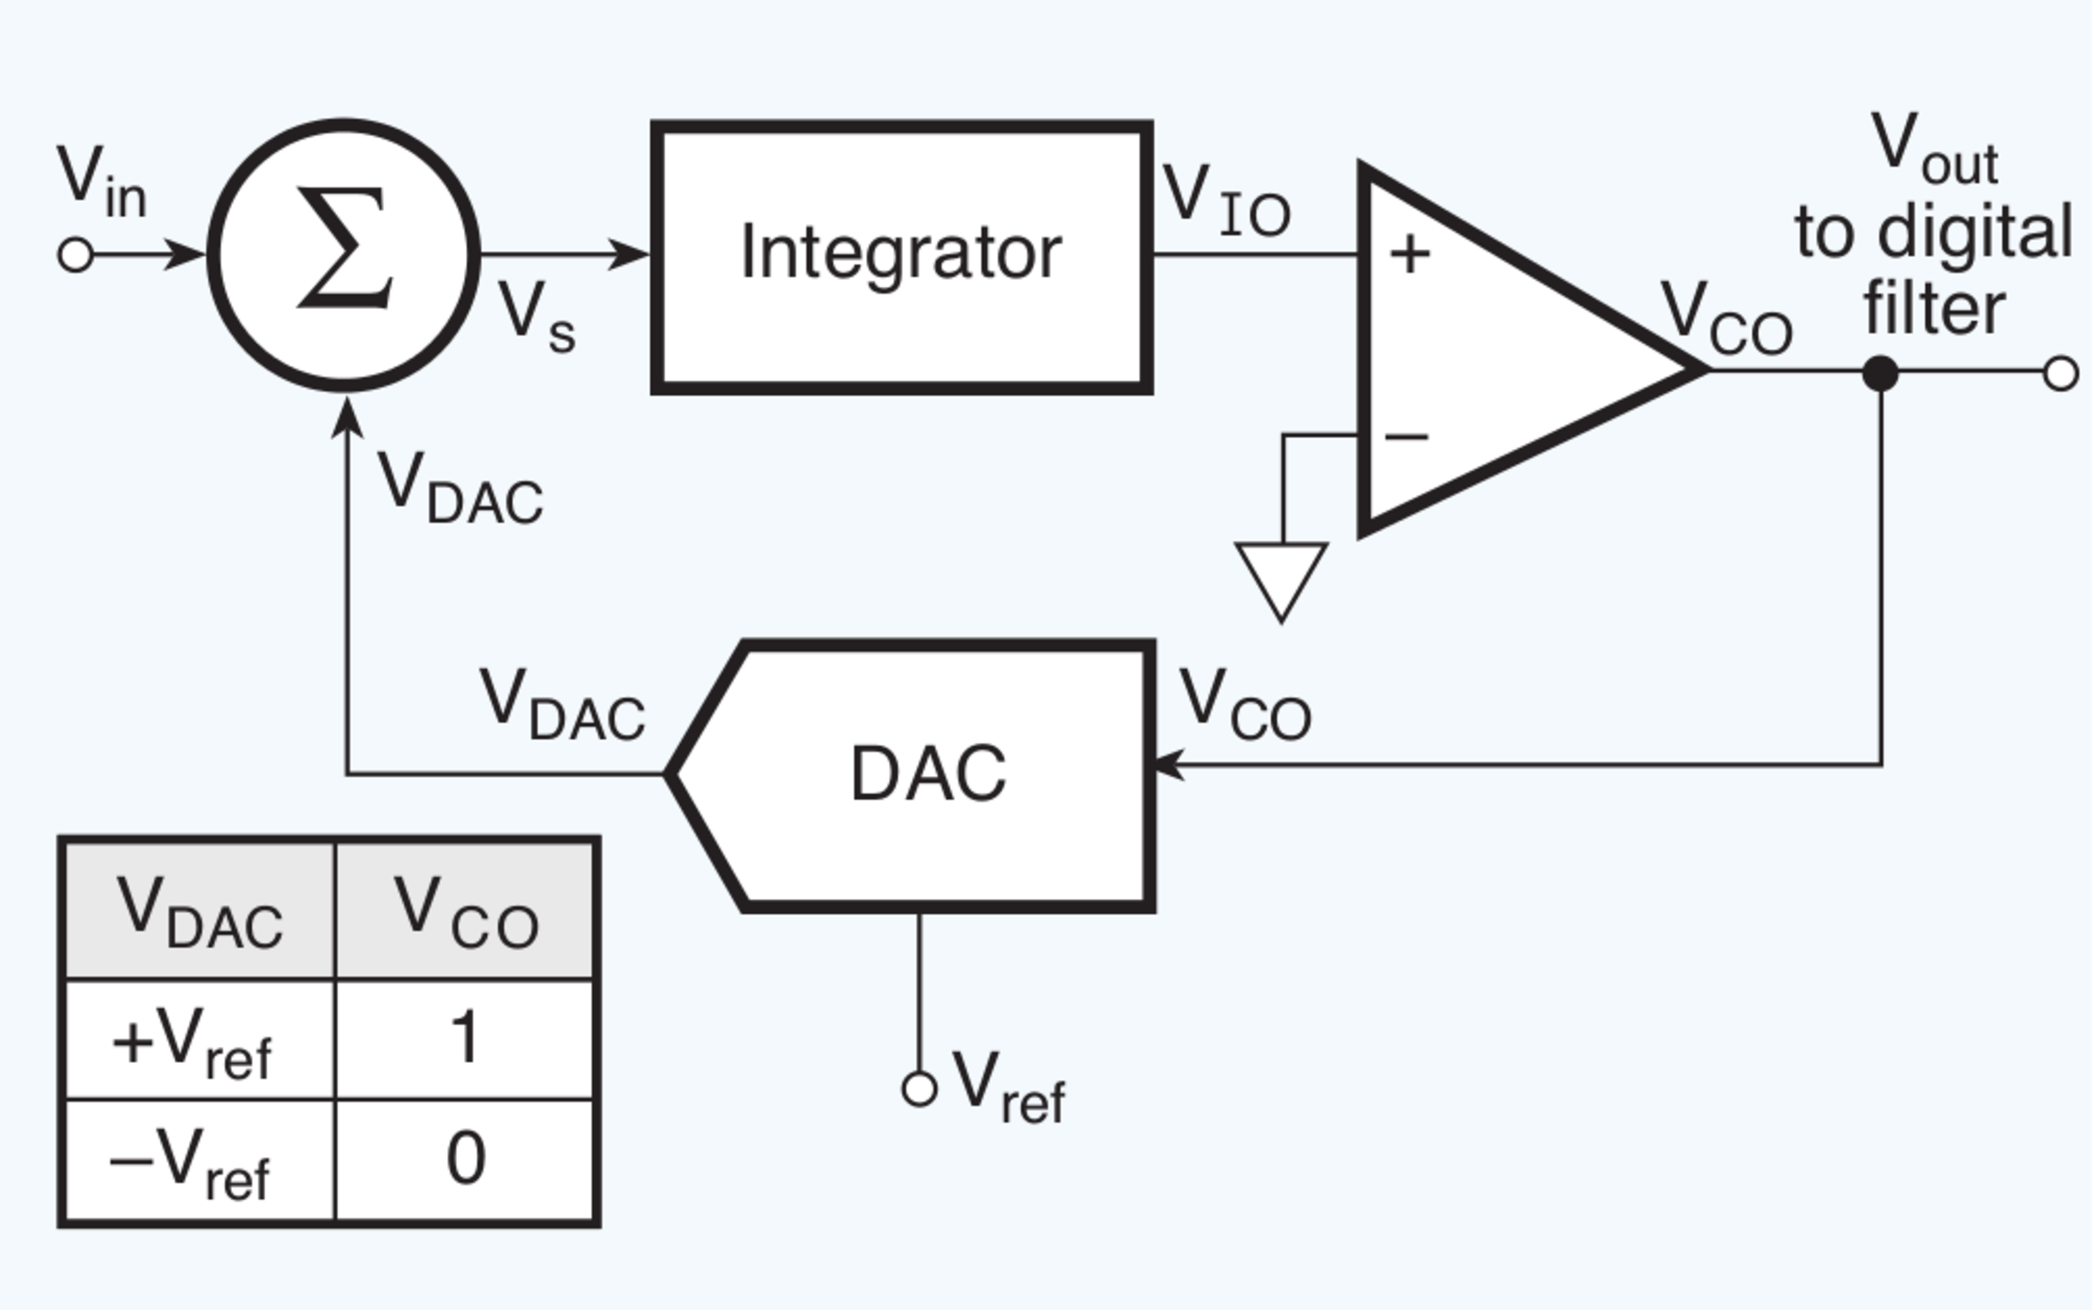
\includegraphics[width=0.8\textwidth]{d3/adc_sigma_delta} \\
      \vspace{5mm}
      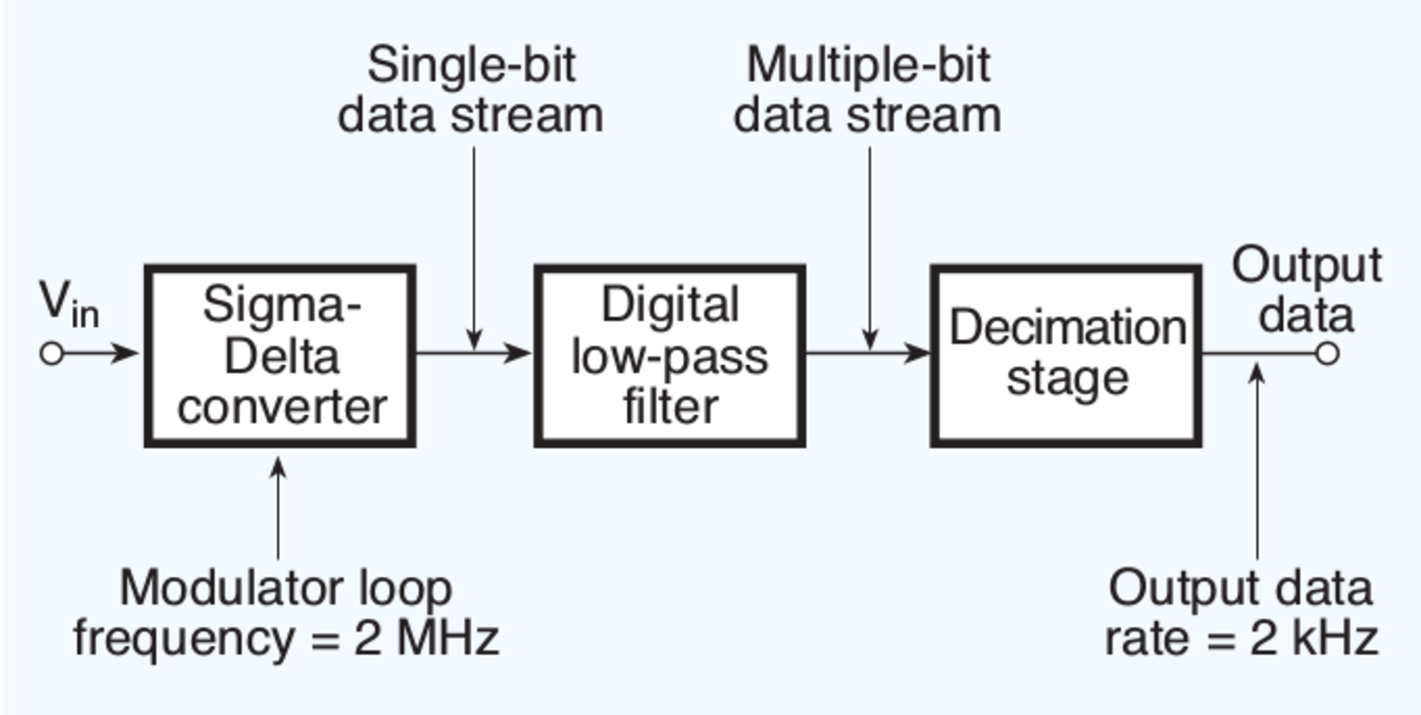
\includegraphics[width=0.8\textwidth]{d3/sigma_delta_w_filter}
  \end{center}
    \end{column}
  \end{columns}
\end{frame}

\subsubsection{Comparación}

\begin{frame}
\frametitle{Comparación}
\begin{center}
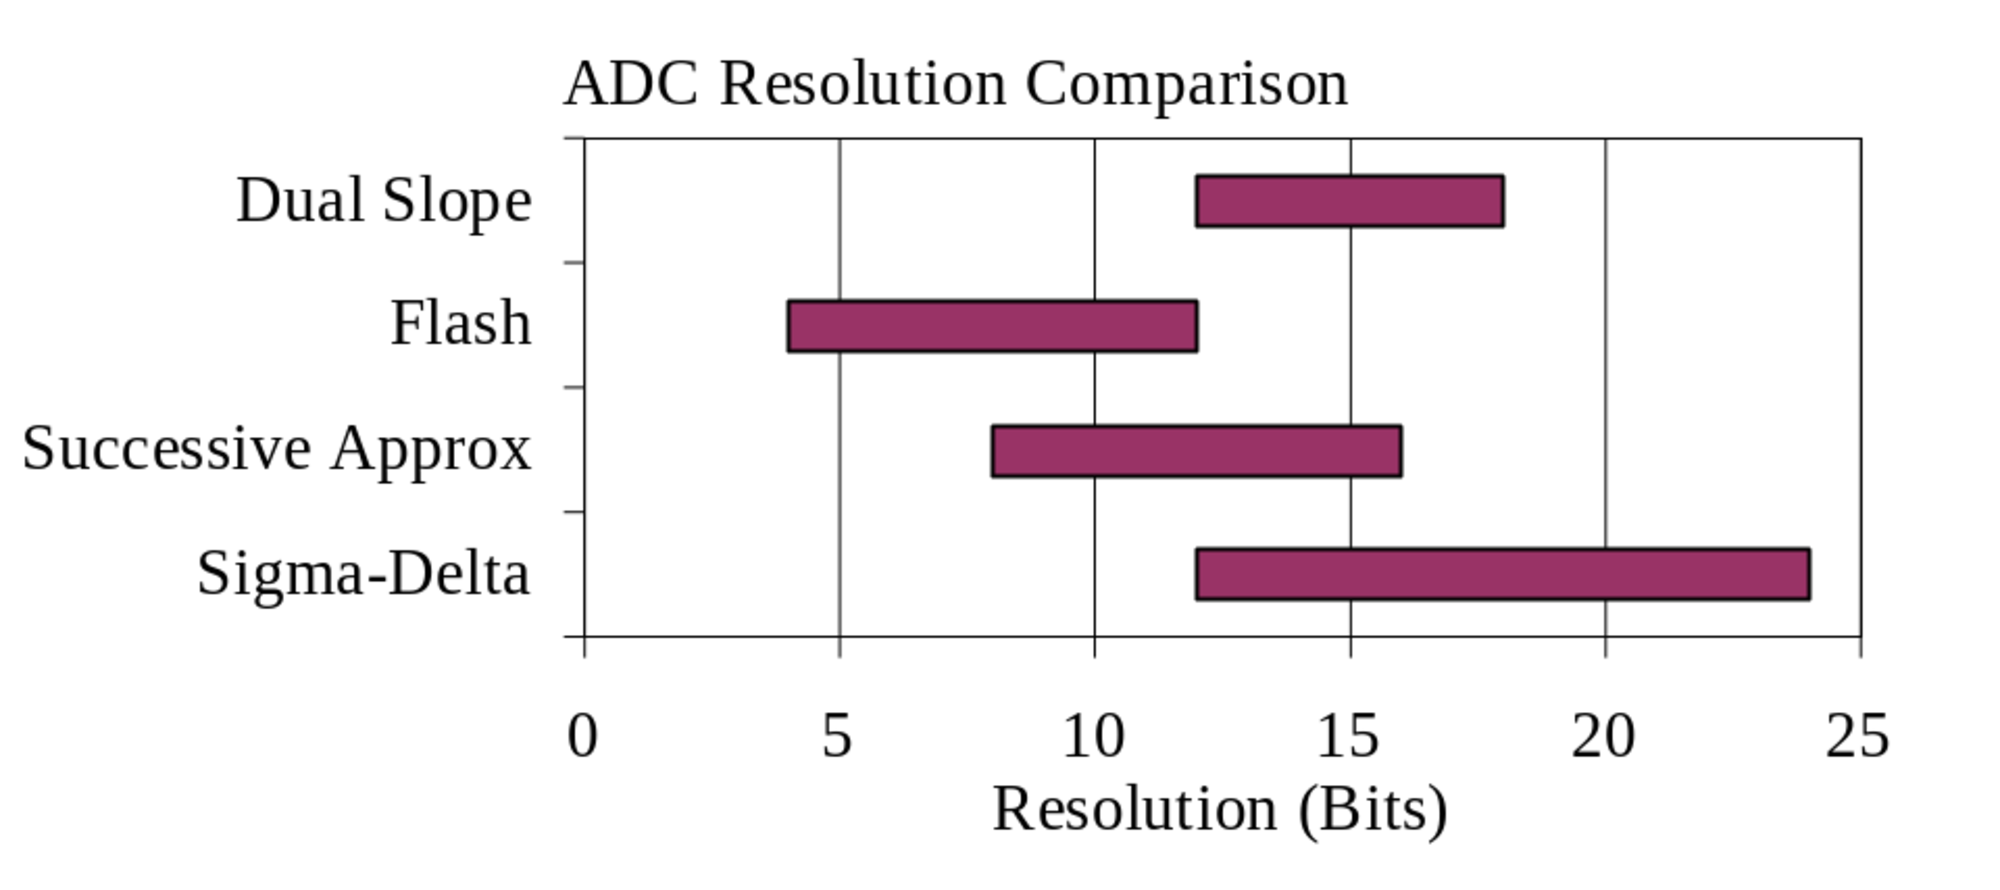
\includegraphics[width=0.7\textwidth]{d3/adc_types_comparison}
\end{center}
\begin{table}[bt]
\begin{tabular}{|l|l|l|} \hline
\textbf{Tipo}    & \bf{Velocidad (relativo)} & \bf{Costo (relativo)} \\ \hline
 Flash            & Muy rápido                 & Alto  \\
 Aprox. Sucesivas & Media - Alta	              & Bajo  \\
 V-f              & Media - Alta	              & Bajo  \\
Doble envolvente & Lento                      & Medio \\
Sigma-Delta      & Lento                      &	Bajo  \\ \hline
\end{tabular}
\end{table}
\end{frame}

\begin{frame}
\frametitle{Comparación}
\begin{center}
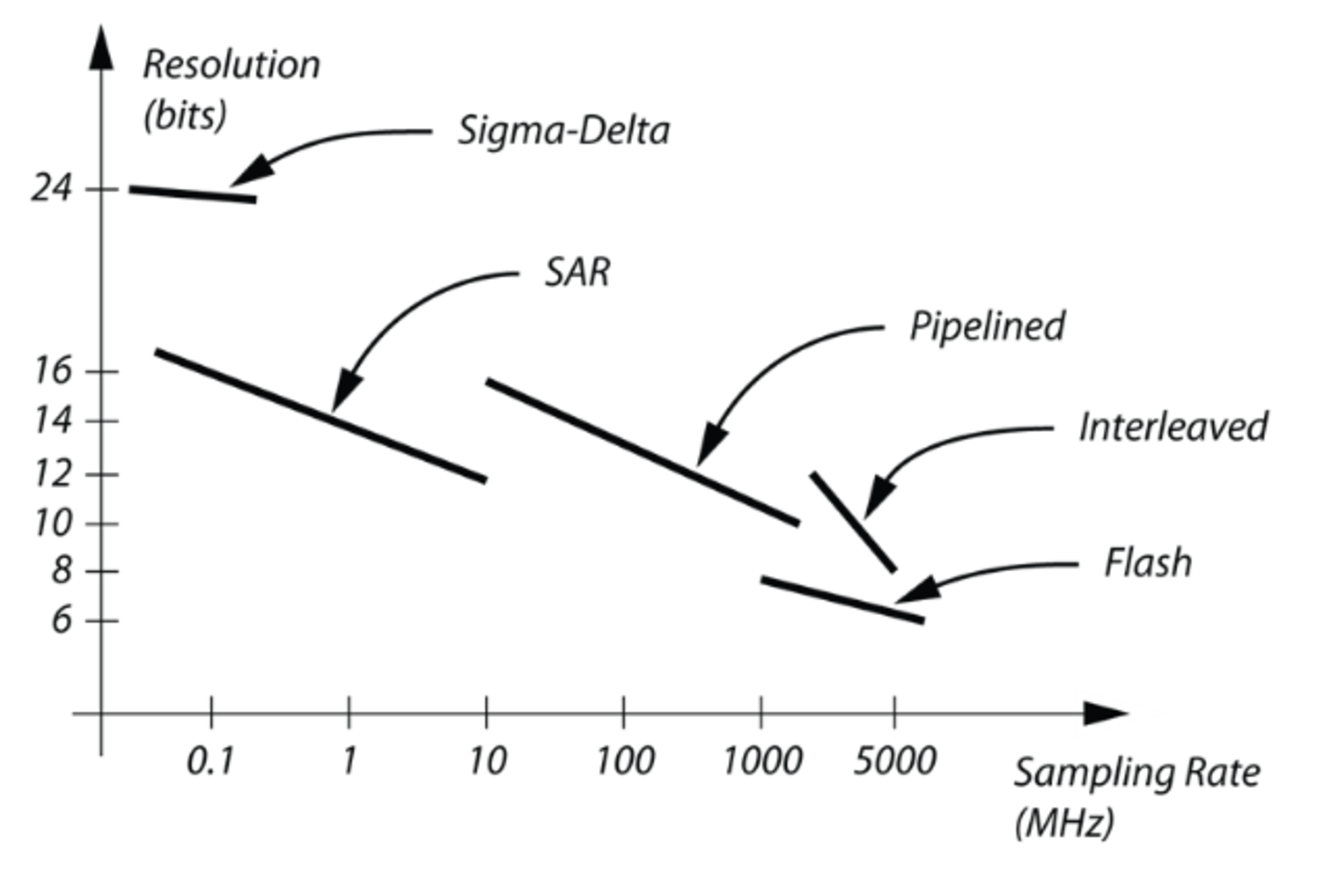
\includegraphics[width=0.8\textwidth]{d3/comparacion_adc_res_vs_frec}
\end{center}
\end{frame}

\begin{frame}
\frametitle{Comparación}
\begin{center}
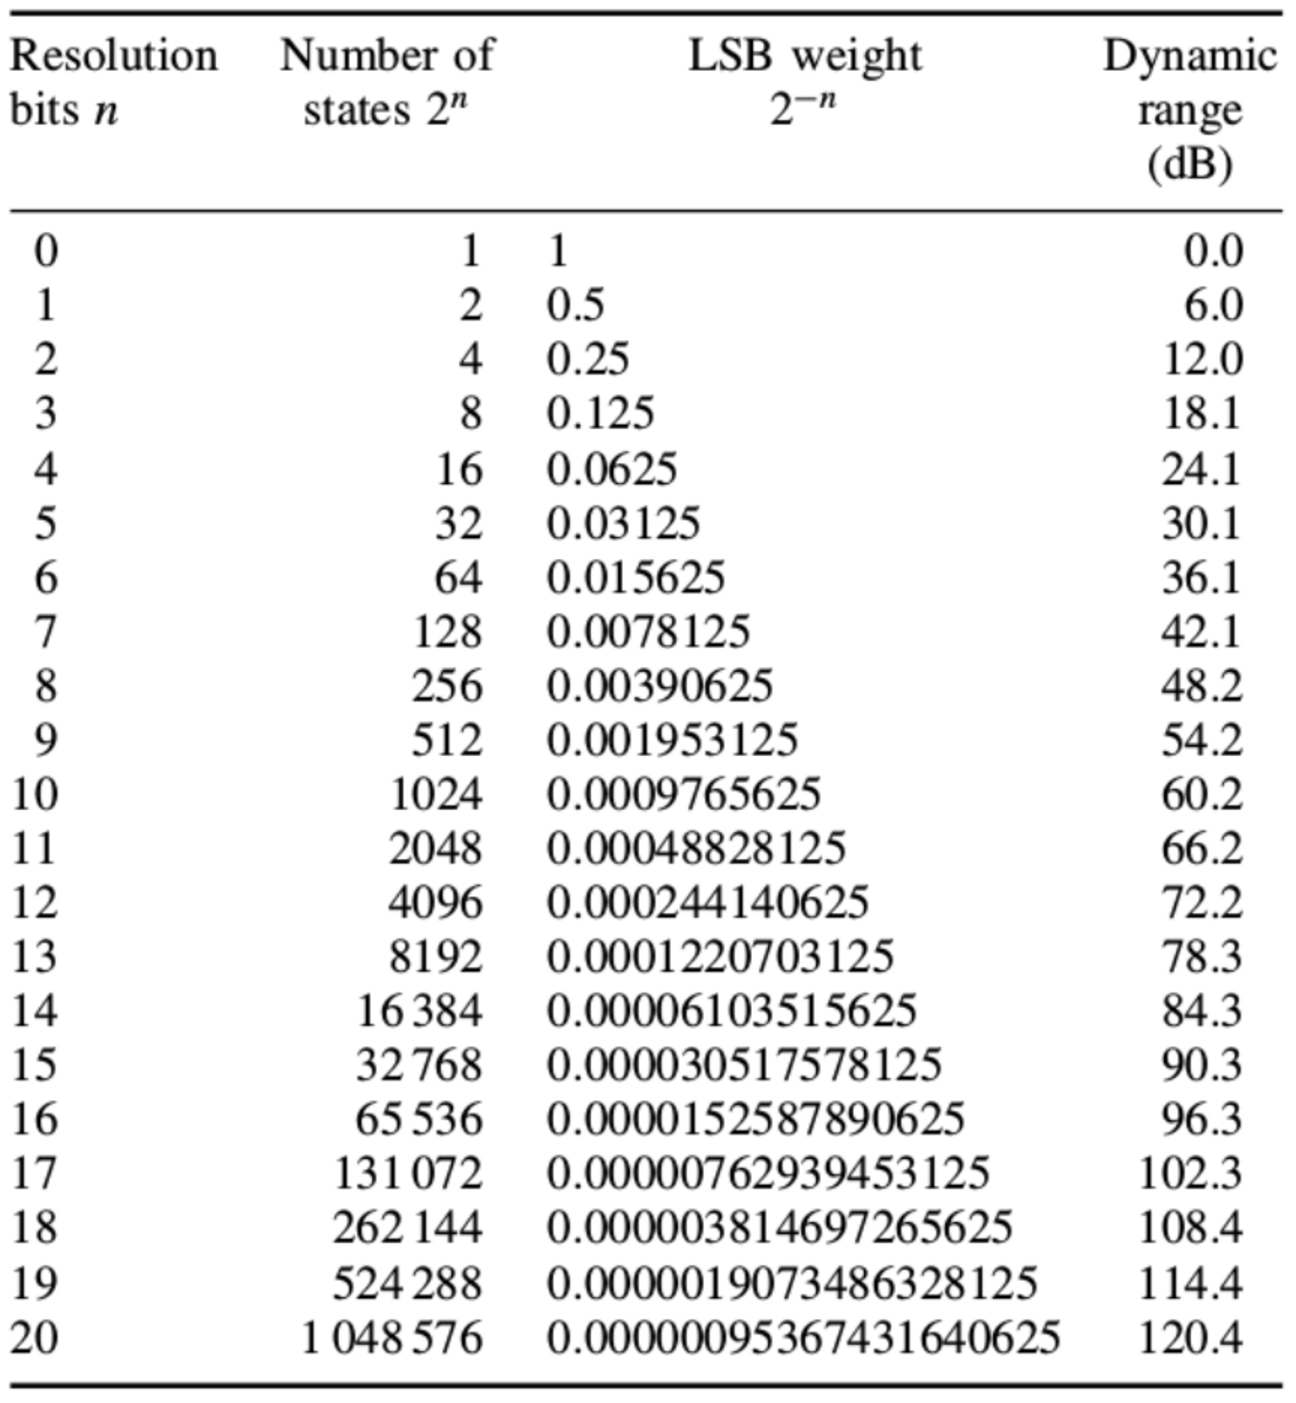
\includegraphics[width=0.5\textwidth]{d3/dinamic_range_adc}
\end{center}
\end{frame}

%------------------------------------------------------------------------------
\section{Precisión vs. Resolución}
%------------------------------------------------------------------------------

\begin{frame}
\frametitle{Precisión vs. Resolución}
\begin{block}{}
\begin{itemize}
\item La precisión es uno de los factores críticos a considerar cuando estamos
especificando un ADC para aplicaciones de medición  
\item Normalmente se confunde precisión con resolución
\item Ambos están relacionados con la calibración, linealidad, pérdida de
códigos y ruido 
\item Cada medición con ADCs tiene errores asociados ({\color{blue}inevitables e
independientes}) que influencian su precisión. Si $\sigma_i$ representa cada uno
de esos errores, el error total va a ser:
$$\sigma_{total} = \sqrt{\sum_i\sigma_i^2}$$  
\end{itemize}
\end{block}
\end{frame}

\begin{frame}
\frametitle{Errores comunes en ADCs}
\begin{center}
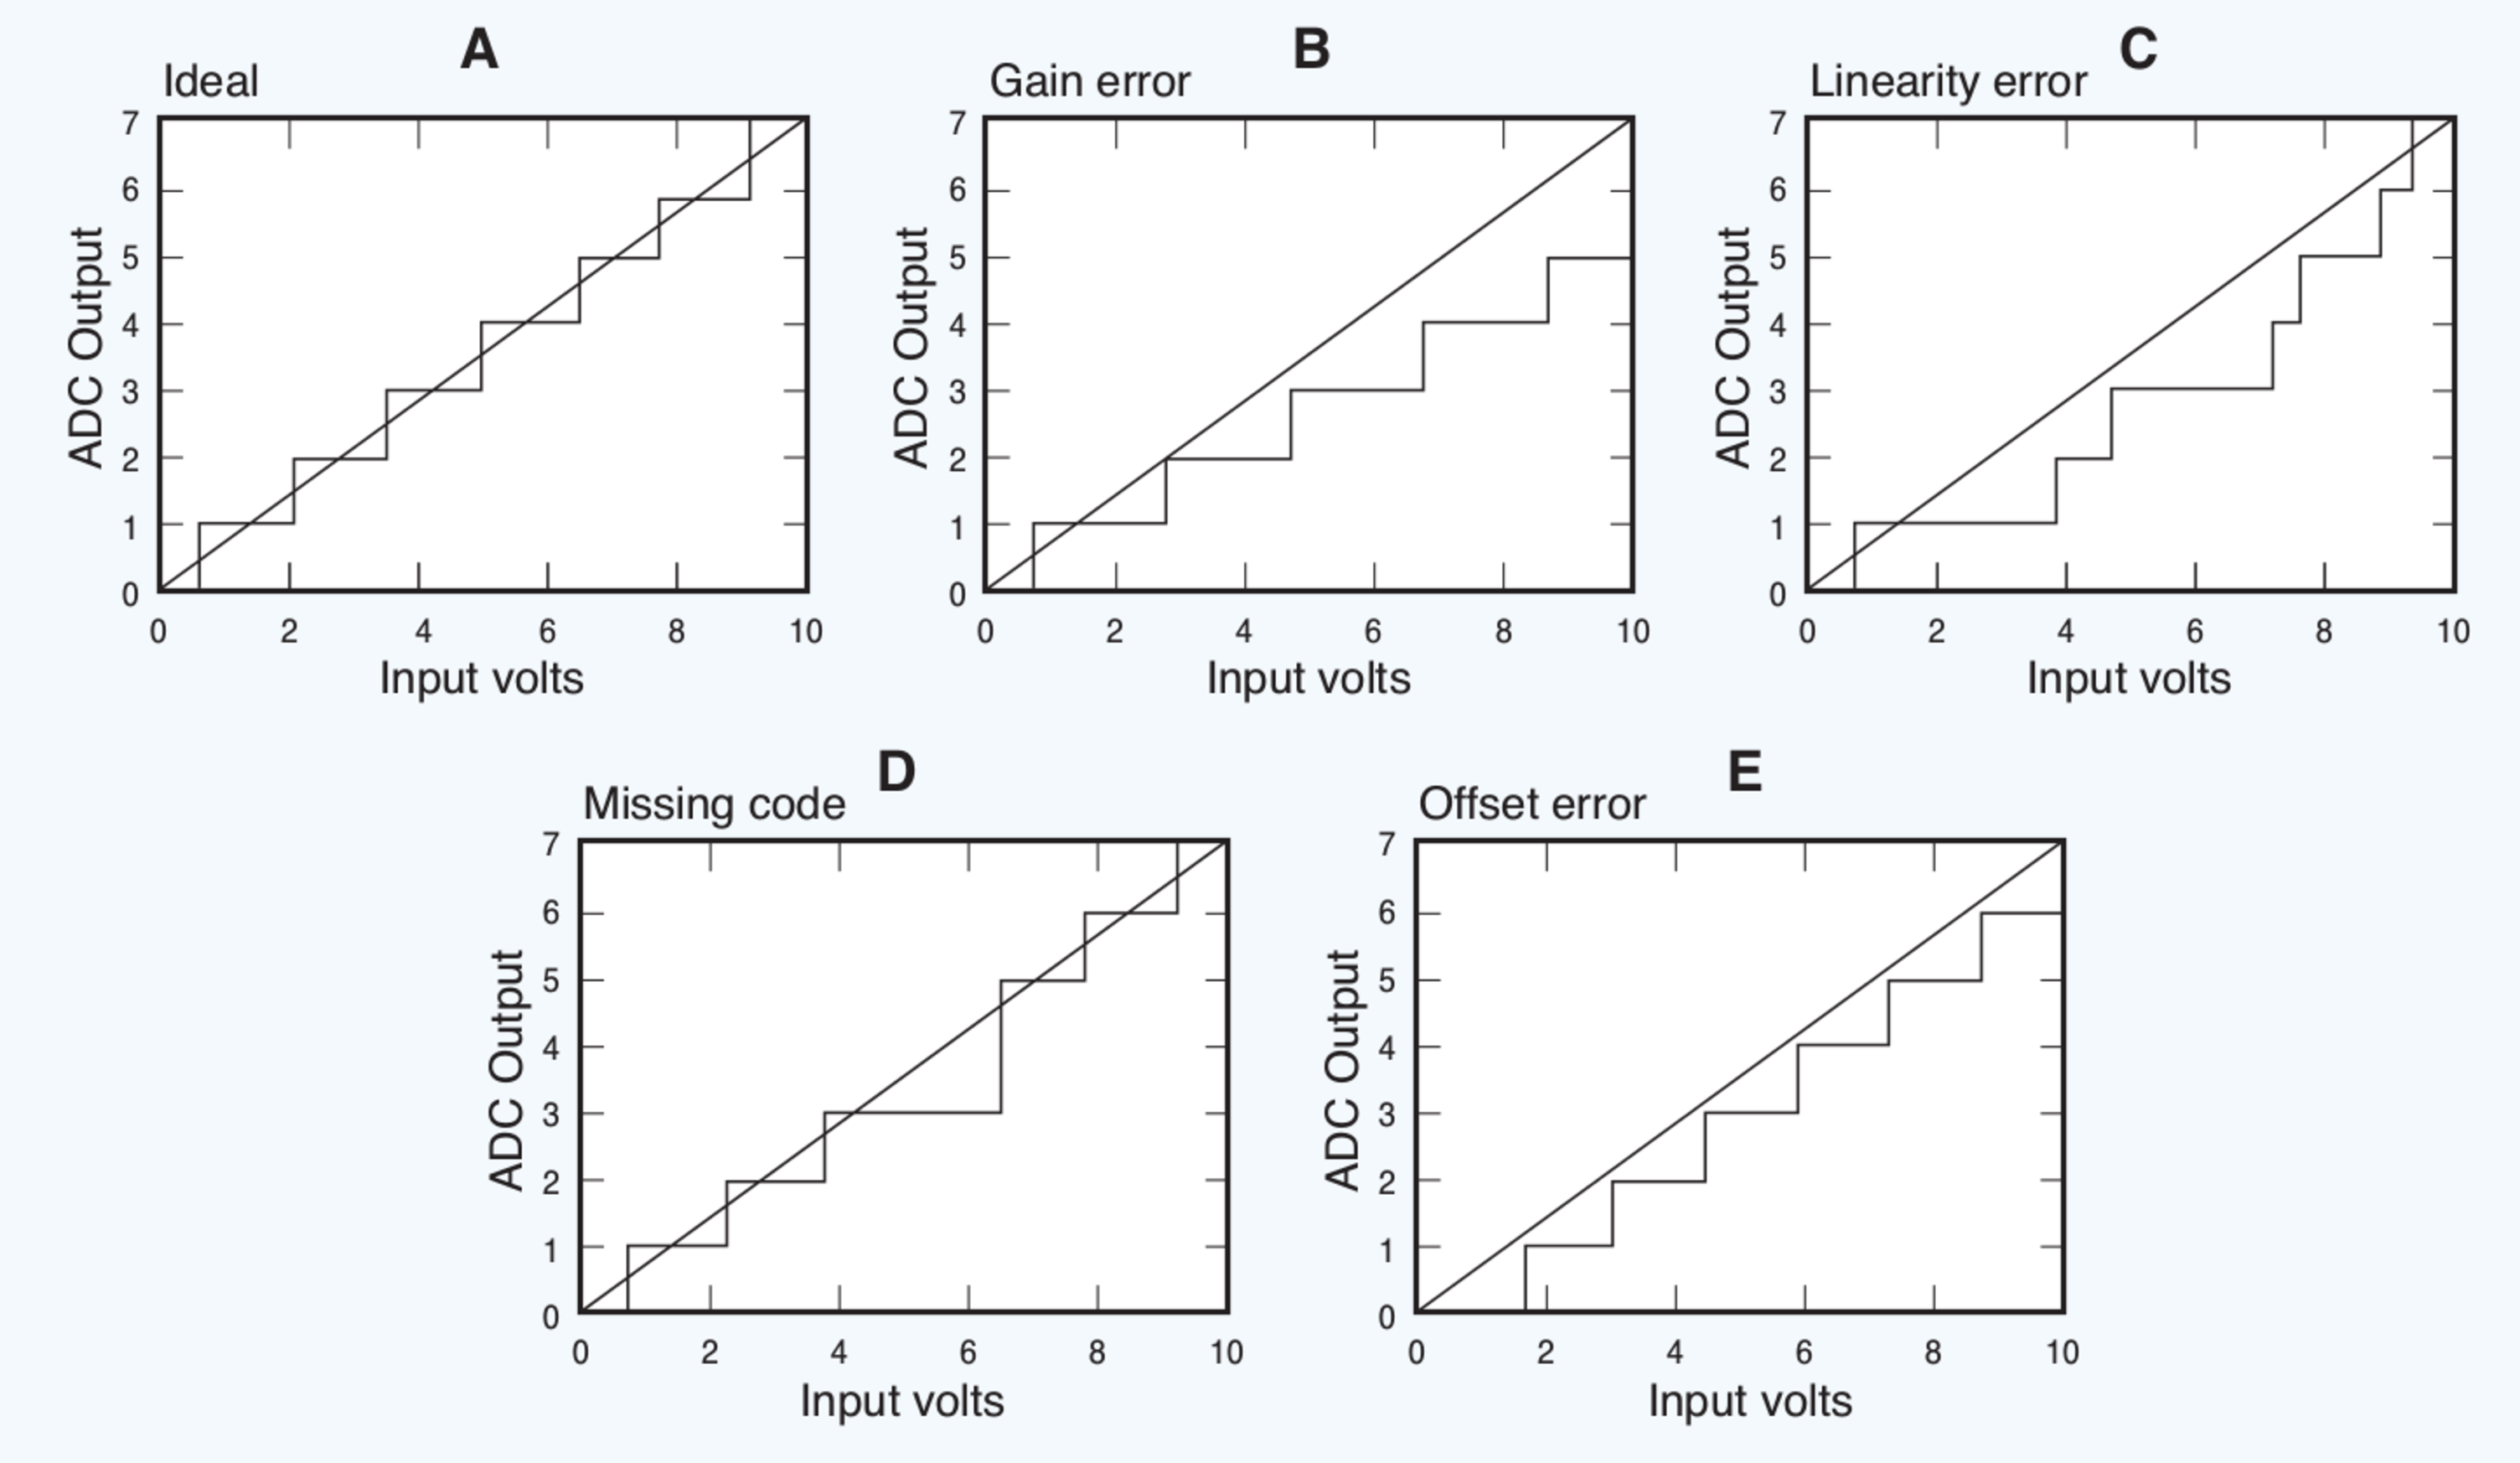
\includegraphics[width=\textwidth]{d3/adc_common_errors}
\end{center}
\end{frame}

\begin{frame}
\frametitle{Error de cuantificación}
\begin{exampleblock}{}
Es el error introducido como consecuencia del proceso de cuantificación
\end{exampleblock}
\begin{exampleblock}{}
\begin{itemize}
\item Depende de la resolución del conversor
\item Tiene un valor fijo: \alert{$1/2\,LSB$}
\item La señal de error de cuantificación es la diferencia entre la
tensión real aplicada y la salida ADC
\item El valor RMS de la señal de cuantificación es
$\frac{1\,LSB}{\sqrt{12}}$
\end{itemize}
\end{exampleblock}
\end{frame}

\subsection{Ejemplo}
%FIXME: ver el ejemplo de AN118 que dice que se puede conseguir 16 bits de resolución con uno de 12 bits
\begin{frame}
%FIXME: este ejemplo está en el Analog Engineer pocket reference pág. 91
\begin{exampleblock}{Ejemplo}
¿Cuál es el SNR para un conversor A/D de 8 bits con $V_{ref} = 5\,V$,
suponiendo ruido de cuantificación?
\end{exampleblock}\pause
\begin{block}{Respuesta}
$SNR = 2^{N-1}\sqrt{6} = 2^{8-1}\sqrt{6} = 314$ \\
\vspace*{5mm}
$SNR_{(dB)} = 20\log{314} = 49.9\,dB$ \\
\vspace*{5mm}
$SNR_{(dB)} = 6.02*8 + 1.76 = 49.9\,dB$ \\
\end{block}
\end{frame}

%%------------------------------------------------------------------------------
%\section{Códigos de representación}
%%------------------------------------------------------------------------------
%\subsection{Ejemplo}
%%------------------------------------------------------------------------------
%\section{Limitaciones en el desempeño}
%%------------------------------------------------------------------------------
%\subsection{Ejemplo}
%------------------------------------------------------------------------------
\section{Mejora en la resolución}
%------------------------------------------------------------------------------

\begin{frame}
\frametitle{Mejora en la resolución por medio de sobremuestreo y promediado}
\begin{exampleblock}{}
En general las aplicaciones requieren una \alert{resolución} basados en el rango
dinámico de la señal y de la relación señal/ruido (SNR) 
\end{exampleblock}
\begin{block}{Puntos centrales}
\begin{itemize}
\item El promediado y sobremuestreo pueden usarse (individualmente o en conjunto) para
mejorar la resolución de la medición, {\color{blue}eliminando la necesidad de recurrir a ADC
más caros}
\item Se mejoran la SNR y la resolución a costa de una mayor carga del CPU y
menor velocidad
\item Se mejora la SNR para el ruido ``blanco''
\end{itemize}
\end{block}
\end{frame}

\begin{frame}
\frametitle{Sobremuestreo y promediado}
\begin{block}{Fuentes de ruido en el conversor A/D}
\begin{itemize}
\item Ruido térmico
\item Ruido shot
\item Variaciones en el voltaje de alimentación
\item Variaciones en el voltaje de referencia
\item Ruido de fase debido a jitter en el reloj
\item Ruido debido al error de cuantificación
\end{itemize}
\end{block}
{
\setbeamercolor{block body}{bg=red!20, fg=blue}
\begin{block}{}
Los ADCs siempre tienen ruido de cuantización, entonces la mejor SNR para una
conversor de datos de n bits viene definida por el ruido de cuantización sin
sobremuestreo
\end{block}}
\end{frame}

\begin{frame}
\frametitle{Sobremuestreo y promediado}
\framesubtitle{Incrementando la resolución de una medición con ADC}
{
\setbeamercolor{block body}{bg=red!20, fg=blue}
\begin{block}{}
Muchas aplicaciones requieren medir dentro de un gran rango dinámico y sin
embargo se desea una alta resolución para medir los cambios en un parámetro.
\end{block}
}
Por ejemplo, un ADC puede medir un rango amplio de temperaturas y a su vez es
preciso que ese ADC responda a cambios de temperatura menores a un grado
centígrado

Ese sistema puede requerir mediciones con una resolución de 16 bits.
{
\setbeamercolor{block body}{bg=green!20}
\begin{block}{}
En lugar de recurrir a un ADC (caro) de 16 bits, uno de 12 bits puede hacer una
medición equivalente a 16 bits con sobremuetreo y promediado 
\end{block}
}
\end{frame}

\begin{frame}
\frametitle{Sobremuestreo y promediado}
\framesubtitle{Calculando los requerimientos para incrementar la resolución por
sobremuestreo}
Nyquist $\rightarrow f_n = 2 f_m$
{
\setbeamercolor{block body}{bg=green!20}
\begin{block}{}
Por cada bit de resolución adicional requerido, la señal debe sobremuestrearse
por un factor de 4
$$\alert{f_{os} = 4^w f_s}$$ 
$f_s = \text{frecuencia original requerida (Nyquist)}$

$w = \text{número de bits adicionales requeridos}$
\end{block}
}
\end{frame}

\begin{frame}
\frametitle{Sobremuestreo y promediado}
\framesubtitle{Calculando los requerimientos para incrementar la resolución por
sobremuestreo}
\begin{block}{Ejemplo}
Asumamos que un sistema mide una temperatura con 12 bits y que toma un valor
cada segundo (1 Hz). Para calcular el sobremuestreo para 16 bits:
$$f_{os} = 4^4\cdot1\,Hz = 256\,Hz$$
Entonces, si muestreamos la temperatura a $f_s = 256\,Hz$, recogeremos
suficientes muestras durante el perído de muestreo requerido para promediarlos y
obtener así una resolución equivalente a 16 bits (\alert{técnica de decimación}) 
\end{block}
\end{frame}

\begin{frame}
\frametitle{Sobremuestreo y promediado}
\framesubtitle{Calculando los requerimientos para incrementar la SNR}
El error de cuantización depende del número de bits de resolución del
conversor. El mejor caso para SNR es calculado como una función del
\textit{número efectivo de bits (ENOB)} de una conversión como sigue:
$$SNR_{dB} = 6.02\cdot\text{ENOB} + 1.76$$

Entonces, si se desea una mejor SNR, se puede usar la ec. anterior para calcular
el ENOB necesario para una SNR específica. Una vez que conocemos el ENOB
necesario, podemos usar la ecuación  $$f_{os} = 4^w f_s$$ para calcular el
sobremuestreo necesario 
\end{frame}

\begin{frame}
\frametitle{Sobremuestreo y promediado}
\framesubtitle{¿Cuándo funcionan?}
La efectividad de este métoddo depende de las fuentes dominantes de ruido en el
sistema.
{
\setbeamercolor{block body}{bg=green!20}
\begin{block}{}
El punto central es que el ruido se pueda modelar como ruido blanco
\end{block}}
\begin{itemize}
\item El ruido debe aproximarse al ruido blanco con densidad espectral de
potencia uniforme en la banda de interés 
\item El ruido en la amplitud debe ser suficiente como para causar que la señal
cambie aleatoriamente de muestra a muestra por una cantidad comparable a al
menos la distancia entre dos códigos adyacentes (es decir, 1 LSB) 
\item La señal de entrada debe poder representarse como una variable aleatoria
que tiene igual probabilidad de existencia en cualquier valor entre dos códigos
ADC adyacentes 
\end{itemize}
\end{frame}


%\subsection{Ejemplo}
%
%%------------------------------------------------------------------------------
%\section{D/A Ideal}
%%------------------------------------------------------------------------------
%
%\subsection{Ejemplo}
%
%\section{Fuentes de ruido}
%
%\begin{frame}
%\frametitle{Hardware}
%\begin{exampleblock}{Características}
%\begin{itemize}
%\item Ruido térmico
%\item Ruido shot
%\item Variaciones en el voltaje de alimentación
%\item Variaciones en el voltaje de referencia
%\item Ruido de fase debido a jitter en el reloj
%\item Error de cuantificación
%\end{itemize}
%\end{exampleblock}
%\end{frame}
%
%%------------------------------------------------------------------------------
%\section{Ruido}
%%------------------------------------------------------------------------------


\begin{frame}
  \begin{center}
    %\huge{¡Muchas Gracias!}
    
\includegraphics[height=0.6\textheight,width=0.65\textwidth]{logos/gracias}
  \end{center}
\end{frame}

\begin{frame}
  \begin{center}
    \huge{¿Preguntas?}\\
    \vspace{5mm}
    
\includegraphics[height=0.4\textheight,width=0.4\textwidth]{logos/preguntas}
  \end{center}
\end{frame}

\end{document}
